% !Mode:: "TeX:UTF-8"
%!TEX program  = xelatex

%% =====================================================================
%% 2024 年高教社杯全国大学生数学建模竞赛
%% B 题：生产过程中的决策问题
%% 论文主文件 —— 基于 cumcmthesis 官方模板
%% =====================================================================

\documentclass[withoutpreface,bwprint]{cumcmthesis}

% 2026C 沿用的扩展宏包
\usepackage{float}        % 浮动体位置控制
\usepackage{caption}      % \captionof 等命令
\usepackage{multirow}
\usepackage{array}
\usepackage{booktabs}
\usepackage{adjustbox}
\usepackage{url}
\usepackage{lmodern}
\usepackage{graphicx}

% 图片搜索路径（覆盖 cls 默认的 figures/，因为图片分散在根目录与各 pN/figures/）
\graphicspath{{../figures/}{../p1/figures/}{../p2/figures/}{../p3/figures/}{../p4/figures/}}

% 标题信息
\title{面向质量不确定性的电子产品抽样验收与多级生产决策优化}
\tihao{B}
\baominghao{}
\schoolname{西安电子科技大学}
\membera{石智中}
\memberb{}
\memberc{}
\supervisor{}
\yearinput{2024}
\monthinput{09}
\dayinput{14}

% 修复 cls 模板中 colorlinks + pdfborder 同时启用导致的 \ref 解析失败
\hypersetup{colorlinks=false}
% 抑制模板中 cleardoublepage 产生的空白页
\let\cleardoublepage\clearpage

% 自定义数学符号（避免与 cls 模板冲突）
\newcommand{\E}{\mathbb{E}}
\newcommand{\BetaDist}{\mathrm{Beta}}
\newcommand{\BinomDist}{\mathrm{Binomial}}
\newcommand{\Beta}{\mathrm{Beta}}
\newcommand{\Binom}{\mathrm{Binomial}}

\begin{document}

\maketitle

\begin{abstract}
针对电子产品生产中供应商验收、零配件检测、成品处置及多级装配质量控制
问题，本文构建"统计验收—期望利润—级联递推—信息价值"一体化模型，
按四道层层递进的子问题展开。

\textbf{针对问题一}，在零次品验收规则下设抽样次品数 $X \sim \mathrm{Bin}(n, p)$，
将可靠度要求转化为精确二项尾概率约束。当标称次品率 $p_0 = 10\%$ 时，
95\% 可靠度拒收对应最小样本量 $n_1 = 29$，90\% 可靠度接收对应 $n_2 = 22$，
闭式公式 $n = \lceil \ln \alpha / \ln(1 - p_0) \rceil$ 与精确搜索完全一致，
且 $n-1$ 不可行证明了最小性。

\textbf{针对问题二}，以"每服务一名客户并最终交付一件合格品"为统一核算
口径，建立含检测、装配、调换、拆解与回收循环的期望利润模型。对 16 种
策略全枚举（$2^4$），辅以 20 万次蒙特卡洛模拟（最大相对误差 1.25\%），
得到六种情形的全局最优解；跨情形遗憾分析表明策略 $0011$ 的最大
遗憾仅 4.83 元/件，为情形未知时的稳健统一方案。

\textbf{针对问题三}，将上述模型推广至 8 零配件、3 半成品、1 成品的 2 道
工序装配网络。定义 16 个二元决策变量，建立自底向上的质量传播与
成本递推公式，证明问题 2 的公式可作为模块逐级嵌套。对 $2^{16} = 65\,536$
种策略全枚举，得到规范最优策略 $11111111\,|\,000\,|\,000\,|\,11$
（8 零配件全检、3 半成品不检、成品检测并拆解），期望利润 66.09 元/件，
成品实际不合格率 $q_f = 0.3439$，模拟相对误差 0.064\%。

\textbf{针对问题四}，将抽样内生化到决策链，引入 Beta--Binomial 后验
更新与样本信息价值 EVSI 框架。定义观测驱动策略
$x^\star(\mathbf{k}, n)$ 与事前价值 $V(n)$，在默认参数下
（$B = 1000$，$d = 2$，$n_{\mathrm{prior}} = 30$）仅情形 2 在 $n^\star = 10$
处取得正的 EVSI（0.049 元/件）。对批量与检测成本的敏感性分析表明，
$B = 10\,000$ 时抽样经济价值显著放大，情形 6 EVSI 最高达 0.65 元/件
（约 6500 元/批）。

\textbf{综上}，本文以精确二项分布、解析期望利润、级联递推与贝叶斯
决策形成统一方法学：问题 1 给出供应商抽样的最小样本量，问题 2、3
在给定质量参数下通过完整枚举选出全局最优，问题 4 反过来回答"抽样
在何种经济参数下值得其成本"。全文方法无概率近似、解析可复核、跨
问题口径一致，可为同类多阶段质量控制问题提供参考。

\keywords{抽样验收\quad 级联递推\quad 期望利润\quad 全枚举\quad 贝叶斯决策\quad 样本信息价值（EVSI）}

\end{abstract}

% 目录
\tableofcontents
\newpage

%% =====================================================================
%% 一、问题重述
%% =====================================================================
\section{问题重述}

\subsection{问题背景}

某电子产品生产企业需要分别采购零配件 1 与零配件 2，经装配得到成品。
在装配过程中，只要任一零配件不合格，成品必然不合格；而当两个零配件均
合格时，由于装配工艺的随机性，所得成品仍可能不合格（次品率记为 $p_0$）。
企业对市场不合格品采取无条件调换策略，因此每一件合格品的交付背后
都隐含着一组检测、装配、退换与拆解决策。

该问题的数学本质是：在质量参数不完全已知条件下，如何在供应商验收、
零配件检测、成品处置与拆解回收之间作出一组最优决策，以最大化企业
期望利润。题目通过四道子问题，将该问题从纯统计判定（问题 1）
扩展到单级生产决策（问题 2）、多级装配网络推广（问题 3），最终将抽样
本身内生化到决策链中（问题 4），由外生质量参数逐步过渡到信息获取
与生产策略的联合优化。

\subsection{问题提出}

\begin{enumerate}
    \item \textbf{供应商抽样验收方案设计}：供应商声称某批零配件的次品率
    不超过标称值 $p_0$，企业准备采用抽样检测方法决定是否接收。需设计
    检测次数尽可能少的抽样方案，使得在 95\% 可靠度下能够拒收次品率
    超标的批次，在 90\% 可靠度下能够接收次品率未超标的批次。

    \item \textbf{两零配件生产决策优化}：已知两种零配件和成品的次品率，
    需对每一零配件及成品是否检测、对不合格成品是否拆解等 4 个 0-1 决策
    作出选择；对表 1 给定的 6 种情形给出具体决策方案、依据与指标。

    \item \textbf{多级装配系统推广}：对 $m$ 道工序、$n$ 个零配件的多级
    装配系统，重复问题 2 的决策框架。图 1 给出 2 道工序、8 个零配件的
    具体网络与表 2 参数，需给出全局最优决策方案。

    \item \textbf{抽样—决策一体化的经济闭环}：若问题 2、3 中的次品率
    本身由抽样检测方法得到（存在估计误差），需将抽样量作为决策变量
    内生化，重新求解问题 2、3，并讨论抽样的经济价值与最优样本量。
\end{enumerate}

\newpage

%% =====================================================================
%% 二、问题分析
%% =====================================================================
\section{问题分析}

\subsection{问题一分析}

问题一的本质是"在可靠度约束下设计最小样本量"的统计判定问题。
与传统的 Neyman--Pearson 假设检验不同，题面的"信度"指代业务上的
判定可靠度：在 $p = p_0$ 处作出拒收（或接收）判定的概率不低
于 95\%（或不高于 10\% 错判率）。这要求将可靠度转化为精确二项分布
的尾概率约束，给出闭式最小样本量公式，并用相邻整数验证最小性。

由于二项分布的尾概率随 $n$ 单调变化，最小样本量的求解可完全通过
闭式公式 $\lceil \ln \alpha / \ln(1 - p_0) \rceil$ 完成，无需数值搜索
或正态近似。问题的关键在于辨析"判定可靠度"与传统显著性检验的区别，
并以精确二项概率而非正态近似统一全文口径。

\subsection{问题二分析}

问题二的核心是"在已知质量参数下选择最优生产与拆解策略"的经济
决策问题。题面给出 4 个 0-1 决策变量（$x_1, x_2, x_3, x_4$），共
$2^4 = 16$ 种策略。题目要求以"每服务一名客户并最终交付一件合格品"
为统一核算口径，由此可建立期望利润解析模型：

\begin{itemize}
    \item 拆解循环与整体重购两种处置分支必须采用相同的产出口径，
    才能使利润可直接比较；
    \item 质量传播决定了实际不合格率 $q$；
    \item 几何级数形式的循环期望成本与首轮成本相耦合，共同决定
    利润函数。
\end{itemize}

由于策略空间小，枚举所有 16 种策略是合理的求解方式，结果可严格
复核。问题二还需通过单参数分岔与跨情形遗憾分析，识别在情形未知
条件下的稳健统一策略。

\subsection{问题三分析}

问题三将问题 2 从"两零配件—成品"的单级结构推广为"八零配件—
三半成品—成品"的多级网络，决策空间扩大为 $2^{16} = 65\,536$。
问题三的关键不在于枚举规模本身，而在于证明问题 2 的质量传播
与循环成本公式可以作为模块逐级嵌套：每个半成品节点都可以视为
问题 2 的递归组合，最终形成自底向上的统一递推。

由于零配件 1--8 的次品率均为 10\%，半成品和成品工艺次品率也
均为 10\%，问题 3 还可作为"质量风险级联放大"的典型案例：
单节点 10\% 的风险经过 4 次组合后使最终成品不合格率达到 34.39\%
（$0.9^4 = 0.6561$ 的反面），多级装配系统因此天然面对分散拦截
与集中兜底之间的权衡。

\subsection{问题四分析}

问题四要求将抽样内生化到决策链，回答"抽多少、观察到什么、据此
如何改变生产决策、信息是否值得其成本"。与前两问不同，这里的
次品率参数本身不确定，观测结果会更新后验认知并改变最优生产
策略，因此抽样量、生产决策与信息价值需要在同一目标函数下联合
求解，本质是一个贝叶斯决策问题。

模型采用 Beta 先验 + Binomial 抽样 + Beta 后验的共轭框架，定义
观测驱动策略 $x^\star(\mathbf{k}, n)$ 与事前价值 $V(n)$，并以
$\mathrm{EVSI} = V(n^\star) - V(0)$ 衡量抽样净价值。问题 4 的核心
结论是：在默认参数下大多数情形不值得抽样（利润平台效应），但
生产批量增大后抽样经济价值显著放大，情形 6 在 $B = 10\,000$、
$d = 5$ 时 EVSI 达 0.65 元/件（$n^\star = 70$），在 $d = 0.5$
时最优抽样量达到扫描上限 $n^\star = 100$。
抽样值不值得做，最终由批量与检测成本决定，而不是由统计精度
单独决定。

%% =====================================================================
%% 三、基本假设
%% =====================================================================
\section{基本假设}

为兼顾建模精度与解析可行性，本文采用以下基本假设，并在
第 \ref{sec:q1}--\ref{sec:q4} 节结合具体问题作适当调整：

\begin{enumerate}
    \item \textbf{独立同分布假设}：同一批零配件内各件质量相互独立，
    批内真实次品率 $p$ 在抽样与生产期间保持不变。
    \item \textbf{检测无误差}：所有检测手段均无误判、漏判，检测
    结果真实反映被检件的质量状态。
    \item \textbf{工艺次品率}：题给成品次品率 $p_0$ 是由装配工艺
    引起的次品率，仅在两个零配件均合格时才会显现，与未检测
    配件的质量风险相互独立。
    \item \textbf{合格品供需匹配}：合格品存在充分需求，可全部按
    市场售价售出，不考虑库存与产能约束。
    \item \textbf{无条件调换}：对市场不合格品企业无条件调换，损失
    固定为 $r$ 元/件（含物流与企业信誉），核算单位为最终向
    客户交付一件合格品。
    \item \textbf{稳态混合假设}：拆解回收件在企业大规模流水线下
    按节点质量分布重新进入生产循环，不追踪单件回收历史。
    \item \textbf{参数独立性}（仅问题 4）：$p_1, p_2, p_0$ 的先验
    相互独立，默认先验等价样本量 $n_{\mathrm{prior}} = 30$；
    批量 $B$ 与单件检测成本 $d$ 为外生参数。
\end{enumerate}

%% =====================================================================
%% 四、符号说明
%% =====================================================================
\section{符号说明}

\begin{center}
\small
\begin{adjustbox}{width=\textwidth}
\begin{tabular}{>{\centering\arraybackslash}p{3.2cm}>{\centering\arraybackslash}p{10cm}}
    \toprule[1.5pt]
    \textbf{符号} & \textbf{意义} \\ \midrule[1pt]
    $p_i,\ p_0$   & 零配件 $i$、装配工艺的次品率，$p_i, p_0 \in [0,1]$ \\
    $q,\ q_i,\ q_f$ & 实际不合格率（叠加未检测配件风险后） \\
    $c_i,\ d_i$   & 零配件 $i$ 的采购单价、检测成本（元/件） \\
    $a,\ d_0,\ f$ & 装配、成品检测、拆解成本（元/次） \\
    $s,\ r$       & 市场售价、调换损失（元/件） \\
    $x_i,\ y_i,\ z_i$ & 检测或拆解二元决策，$\{0,1\}$ \\
    $n,\ k$       & 抽样量、观察到的次品数（非负整数） \\
    $B$           & 每批生产数量（件/批） \\
    $\pi$         & 每服务一个客户的期望利润（元/件合格品） \\
    $V(n)$        & 扣除抽样成本后的事前期望价值（元/件） \\
    $\mathrm{EVSI}$ & 最优抽样相对不抽样的净价值（元/件） \\
    \bottomrule[1.5pt]
\end{tabular}
\end{adjustbox}
\end{center}

%% =====================================================================
%% 五、模型建立与求解
%% =====================================================================
\section{模型建立与求解}

%% ---------- 问题一 ----------
\subsection{问题一的建模与求解}
\label{sec:q1}

\subsubsection{模型构建}

\textbf{1. 随机变量与零次品验收规则}

设从一批零配件中抽检 $n$ 件，记其次品数为
\begin{equation}
    X \sim \mathrm{Bin}(n, p).
\end{equation}
在零次品验收规则下：
\begin{equation}
    X = 0 \Rightarrow \text{接收},\qquad
    X \geq 1 \Rightarrow \text{拒收}.
\end{equation}
由此接收概率与拒收概率分别为
\begin{equation}
    P(\text{接收} \mid p) = (1 - p)^n, \qquad
    P(\text{拒收} \mid p) = 1 - (1 - p)^n.
\end{equation}

\textbf{2. 两类可靠度约束}

情形一（95\% 可靠度拒收）要求在边界 $p = p_0$ 处拒收概率不低于
$1 - \alpha_1 = 95\%$：
\begin{equation}
    1 - (1 - p_0)^n \geq 1 - \alpha_1
    \;\Longleftrightarrow\;
    n \geq \frac{\ln \alpha_1}{\ln(1 - p_0)}.
\end{equation}

情形二（90\% 可靠度接收）要求零次品接收事件在 $p = p_0$ 处的
概率不超过 $\alpha_2 = 10\%$：
\begin{equation}
    (1 - p_0)^n \leq \alpha_2
    \;\Longleftrightarrow\;
    n \geq \frac{\ln \alpha_2}{\ln(1 - p_0)}.
\end{equation}

\textbf{3. 闭式最小样本量}

由于 $n$ 必须为正整数，最小样本量为
\begin{equation}
    n_1 = \left\lceil \frac{\ln \alpha_1}{\ln(1 - p_0)} \right\rceil, \qquad
    n_2 = \left\lceil \frac{\ln \alpha_2}{\ln(1 - p_0)} \right\rceil.
    \label{eq:q1-closed}
\end{equation}

\subsubsection{求解方法}

代入 $p_0 = 0.10$、$\alpha_1 = 0.05$、$\alpha_2 = 0.10$，由
\cref{eq:q1-closed} 直接得
\begin{equation}
    n_1 = \left\lceil \frac{\ln 0.05}{\ln 0.90} \right\rceil
        = \left\lceil 28.43 \right\rceil = 29, \qquad
    n_2 = \left\lceil \frac{\ln 0.10}{\ln 0.90} \right\rceil
        = \left\lceil 21.85 \right\rceil = 22.
\end{equation}

\subsubsection{结果分析}

\textbf{1. 主结果与最小性验证}

\begin{table}[htbp]
\centering
\caption{问题 1 两种抽样方案及最小性验证}
\label{tab:q1-result}
\small
\begin{tabular}{@{}p{2.4cm}p{1.6cm}p{4.0cm}p{5.0cm}@{}}
\toprule[1.5pt]
情形 & 最小样本量 & 边界概率 & 最小性验证 \\
\midrule[1pt]
95\% 可靠度拒收 & \textbf{29} &
$P(\text{拒收}\mid p_0)=0.9529$ &
$n=28$ 时 $P=0.9477<95\%$ \\
90\% 可靠度接收 & \textbf{22} &
$P(\text{接收}\mid p_0)=0.0985$，可靠度 $0.9015$ &
$n=21$ 时 $P=0.1094>10\%$ \\
\bottomrule[1.5pt]
\end{tabular}
\end{table}

\begin{figure}[htbp]
    \centering
    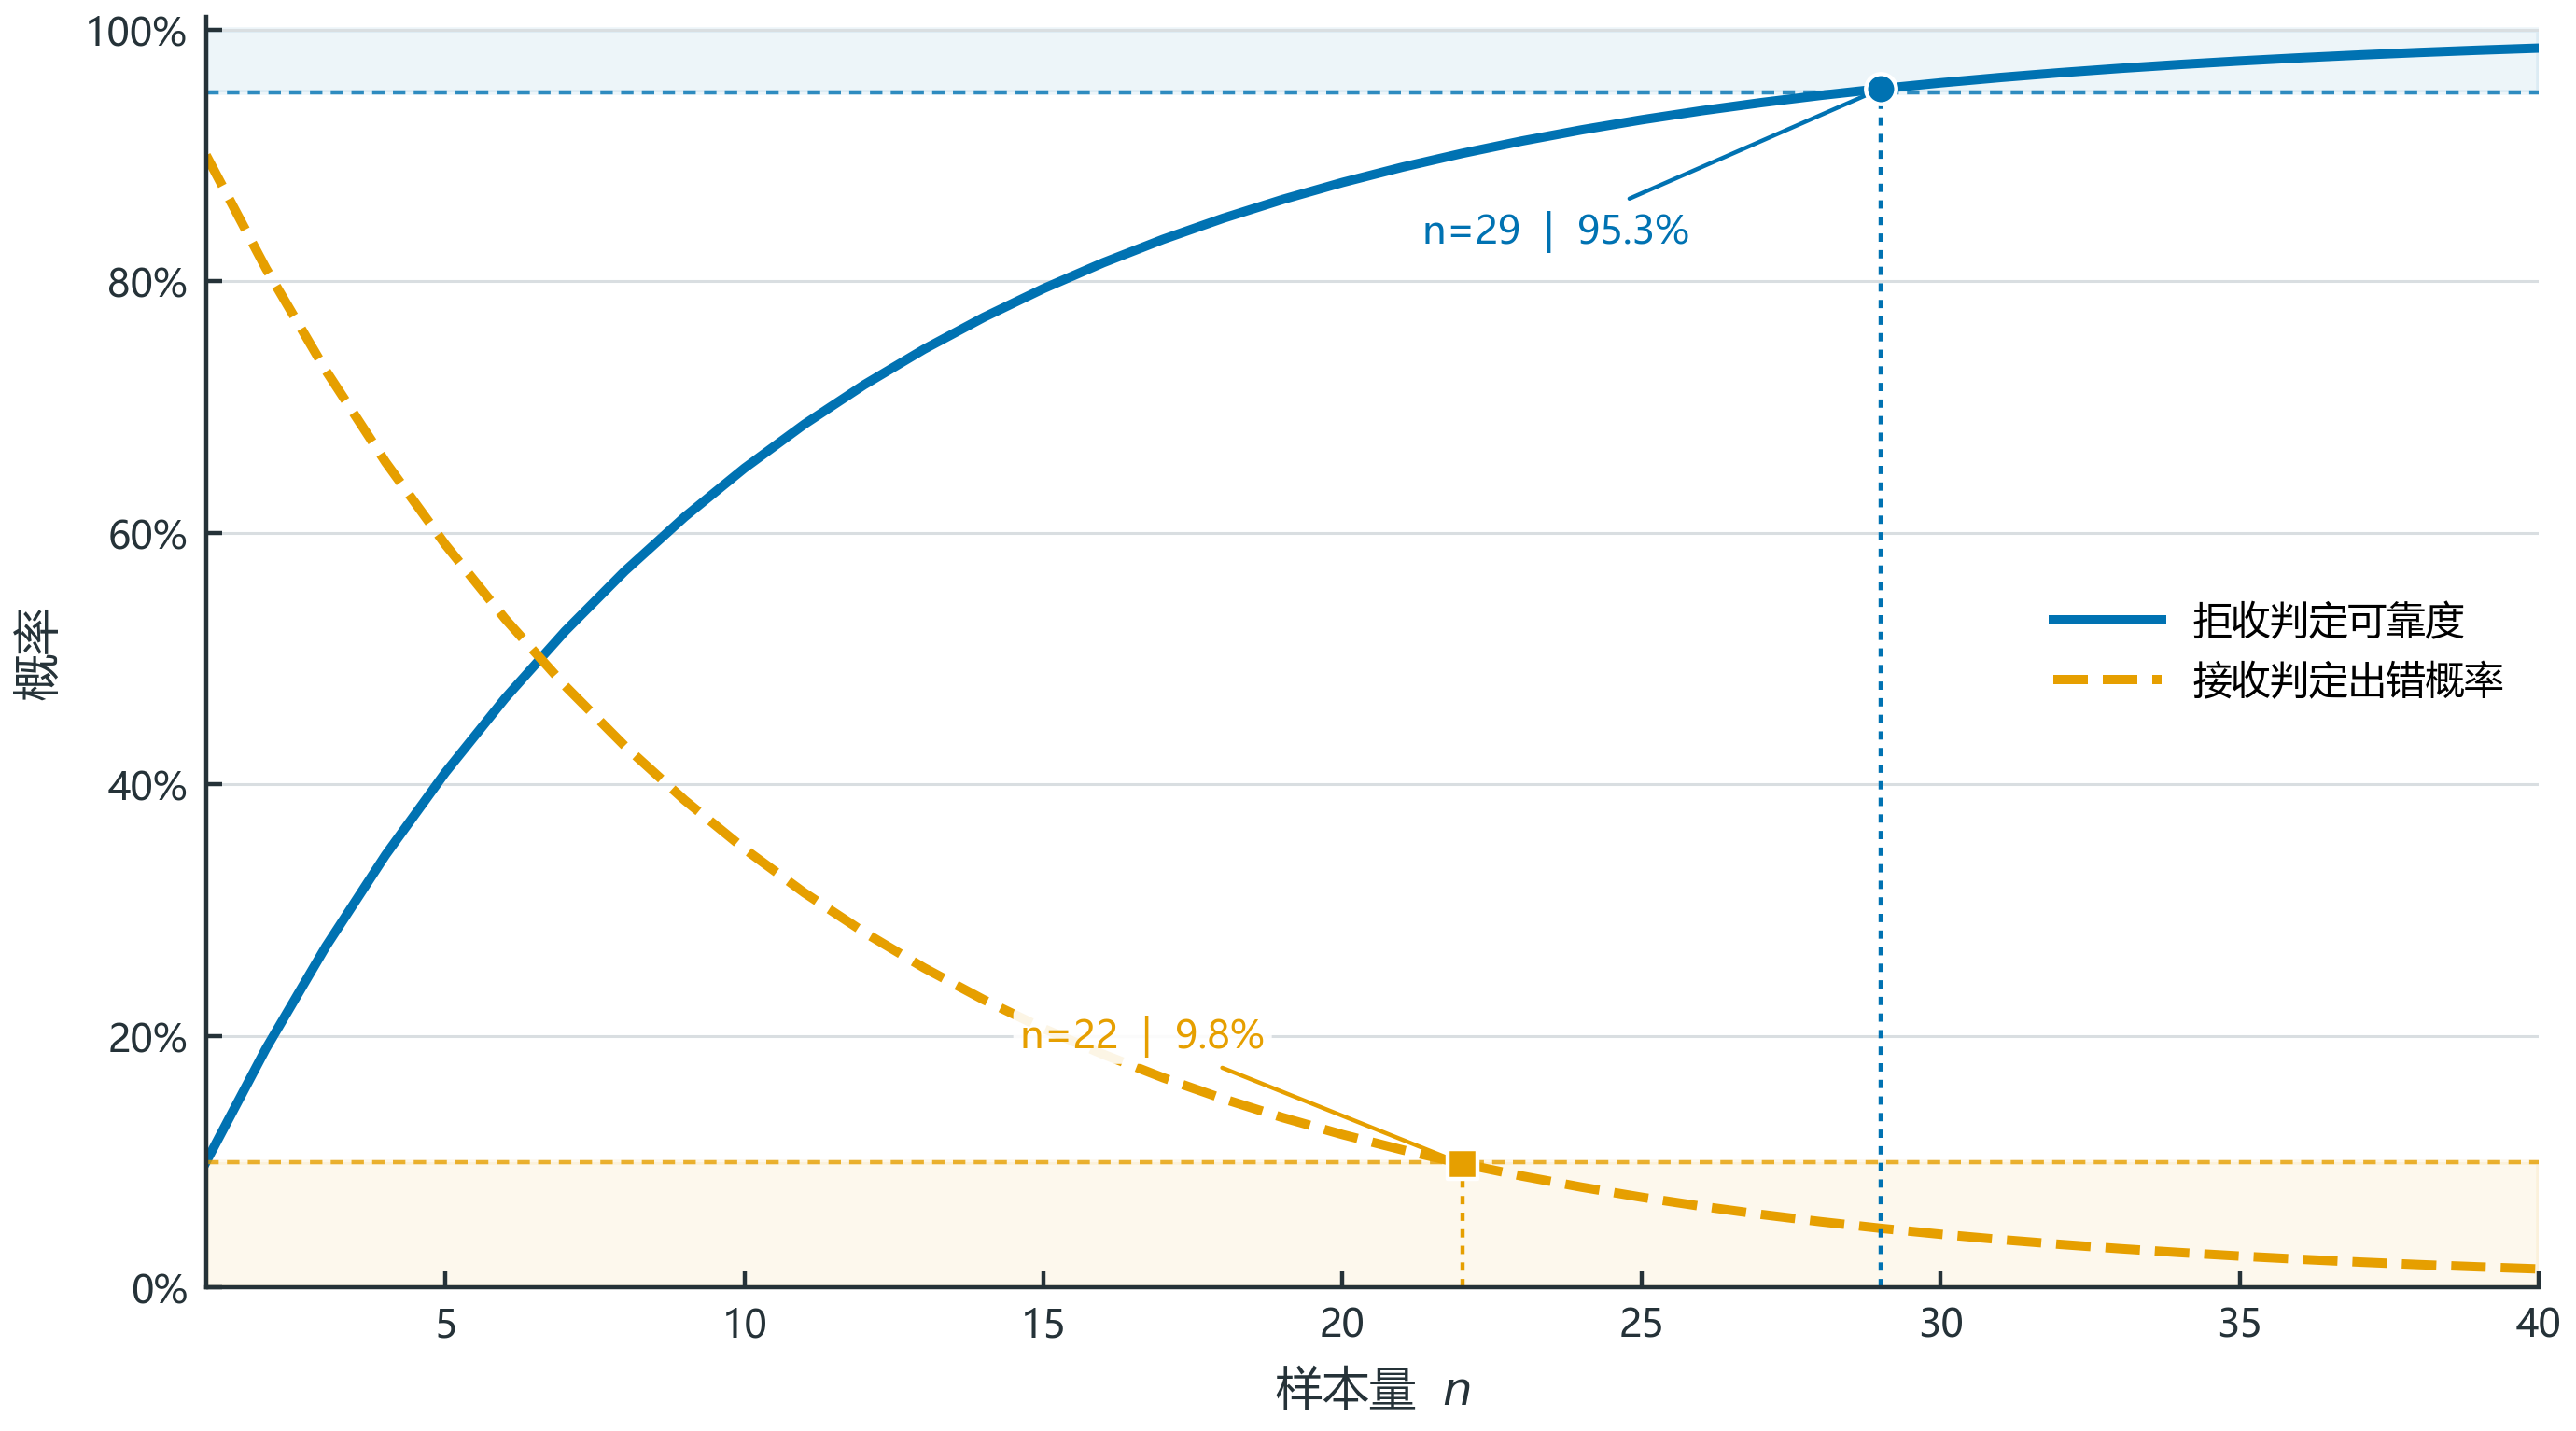
\includegraphics[width=0.92\textwidth]{fig2_reliability_vs_n.png}
    \caption{抽样量 $n$ 与判定可靠度的关系。随着 $n$ 增大，拒收判定可靠度
    $1 - (1-0.10)^n$ 单调上升并穿越 95\% 阈值（对应 $n_1 = 29$），
    接收出错概率 $(1-0.10)^n$ 单调下降并穿越 10\% 阈值（对应 $n_2 = 22$）。
    两曲线与各自阈值的交点同时给出了全局最小整数解。}
    \label{fig:q1-reliability}
\end{figure}

\textbf{2. OC 曲线与方案性能}

验收方案的操作特性函数为 $L(p) = (1 - p)^n$。在 $p = p_0$
处，$n = 29$ 与 $n = 22$ 方案的接收概率分别为 4.71\% 与 9.85\%，
可见较大样本量对高次品率批次更敏感，但同时也降低了合格批次
的接收概率。

\textbf{3. 标称次品率敏感性}

由闭式公式可知，允许的标称次品率越低，为维持同等可靠度所需
样本量越大。当 $p_0 \to 0$ 时，$\ln(1 - p_0) \approx -p_0$，
故 $n \approx -\ln \alpha / p_0$。

\begin{table}[htbp]
\centering
\caption{标称次品率 $p_0$ 在 1\%--20\% 区间的最小样本量（精确二项搜索）}
\label{tab:q1-p0-sensitivity}
\small
\begin{tabular}{@{}lcccccccc@{}}
\toprule[1.5pt]
$p_0$ & 1\% & 2\% & 5\% & 10\% & 15\% & 20\% \\
\midrule[1pt]
$n_1$（95\% 拒收）  & 299 & 149 & 59  & \textbf{29} & 19 & 14 \\
$n_2$（90\% 接收）  & 230 & 114 & 45  & \textbf{22} & 14 & 10 \\
\bottomrule[1.5pt]
\end{tabular}
\end{table}

$p_0$ 从 1\% 升到 20\% 时，$n_1$ 从 299 降至 14（约 21 倍），
$n_2$ 从 230 降至 10（约 23 倍）。标称值越低，同等可靠度下
所需样本越多：5\% 的标称值使 $n_1$ 达到 59，约为 10\% 时
29 的两倍。

\subsubsection{模型检验}

\textbf{1. 闭式公式与精确搜索的一致性}

对 $n = 1, 2, \ldots, 100$ 进行精确二项搜索，得到的最小
样本量与闭式公式完全一致。两种方法独立实现但结果相同，
表明本文求解过程无计算错误。

\textbf{2. 统计口径辨析}

本章采用的"判定可靠度"解释不同于标准 Neyman--Pearson 检验
中的"显著性水平"。将 $H_0: p \leq p_0$ 严格作为原假设时，
在 $p = p_0$ 处以 95\% 概率拒绝 $H_0$ 不符合通常的第一类错误
控制语义。本文因此将其表述为零次品验收规则下的可靠度约束，
避免与传统假设检验概念混用。

\textbf{3. SPRT 扩展的定位}

Wald 序贯概率比检验（SPRT）可作为固定样本量方案的方法扩展
（详见附录 \ref{app:sprt}）。SPRT 在 $p$ 明显优于或劣于 $p_0$
的区域可减少平均抽样次数，但在接近 $p_0$ 的难判区域，期望
抽样次数可能高于固定方案；且 SPRT 复杂度更高、需要事先指定
备择点与两类错误率，不符合题面"以尽量少的抽检次数决定是否
接收"的最简化要求，故不作为主方法。

\subsubsection{单调性与信度敏感性检验}

闭式公式 $n = \lceil \ln(1 - c) / \ln(1 - p_0) \rceil$（$c$ 为信度，
$p_0$ 为标称次品率）蕴含两条单调性质：$n$ 对 $c$ 单调不减（信度
越高越需多抽）、$n$ 对 $p_0$ 单调不增（标称值越严越需多抽）。
对信度 $c$ 在 0.80--0.99 步长 0.005 上扫描，两条差分性质均通过
检验（$n$ 严格非降或非增），未出现反例。

\begin{figure}[htbp]
    \centering
    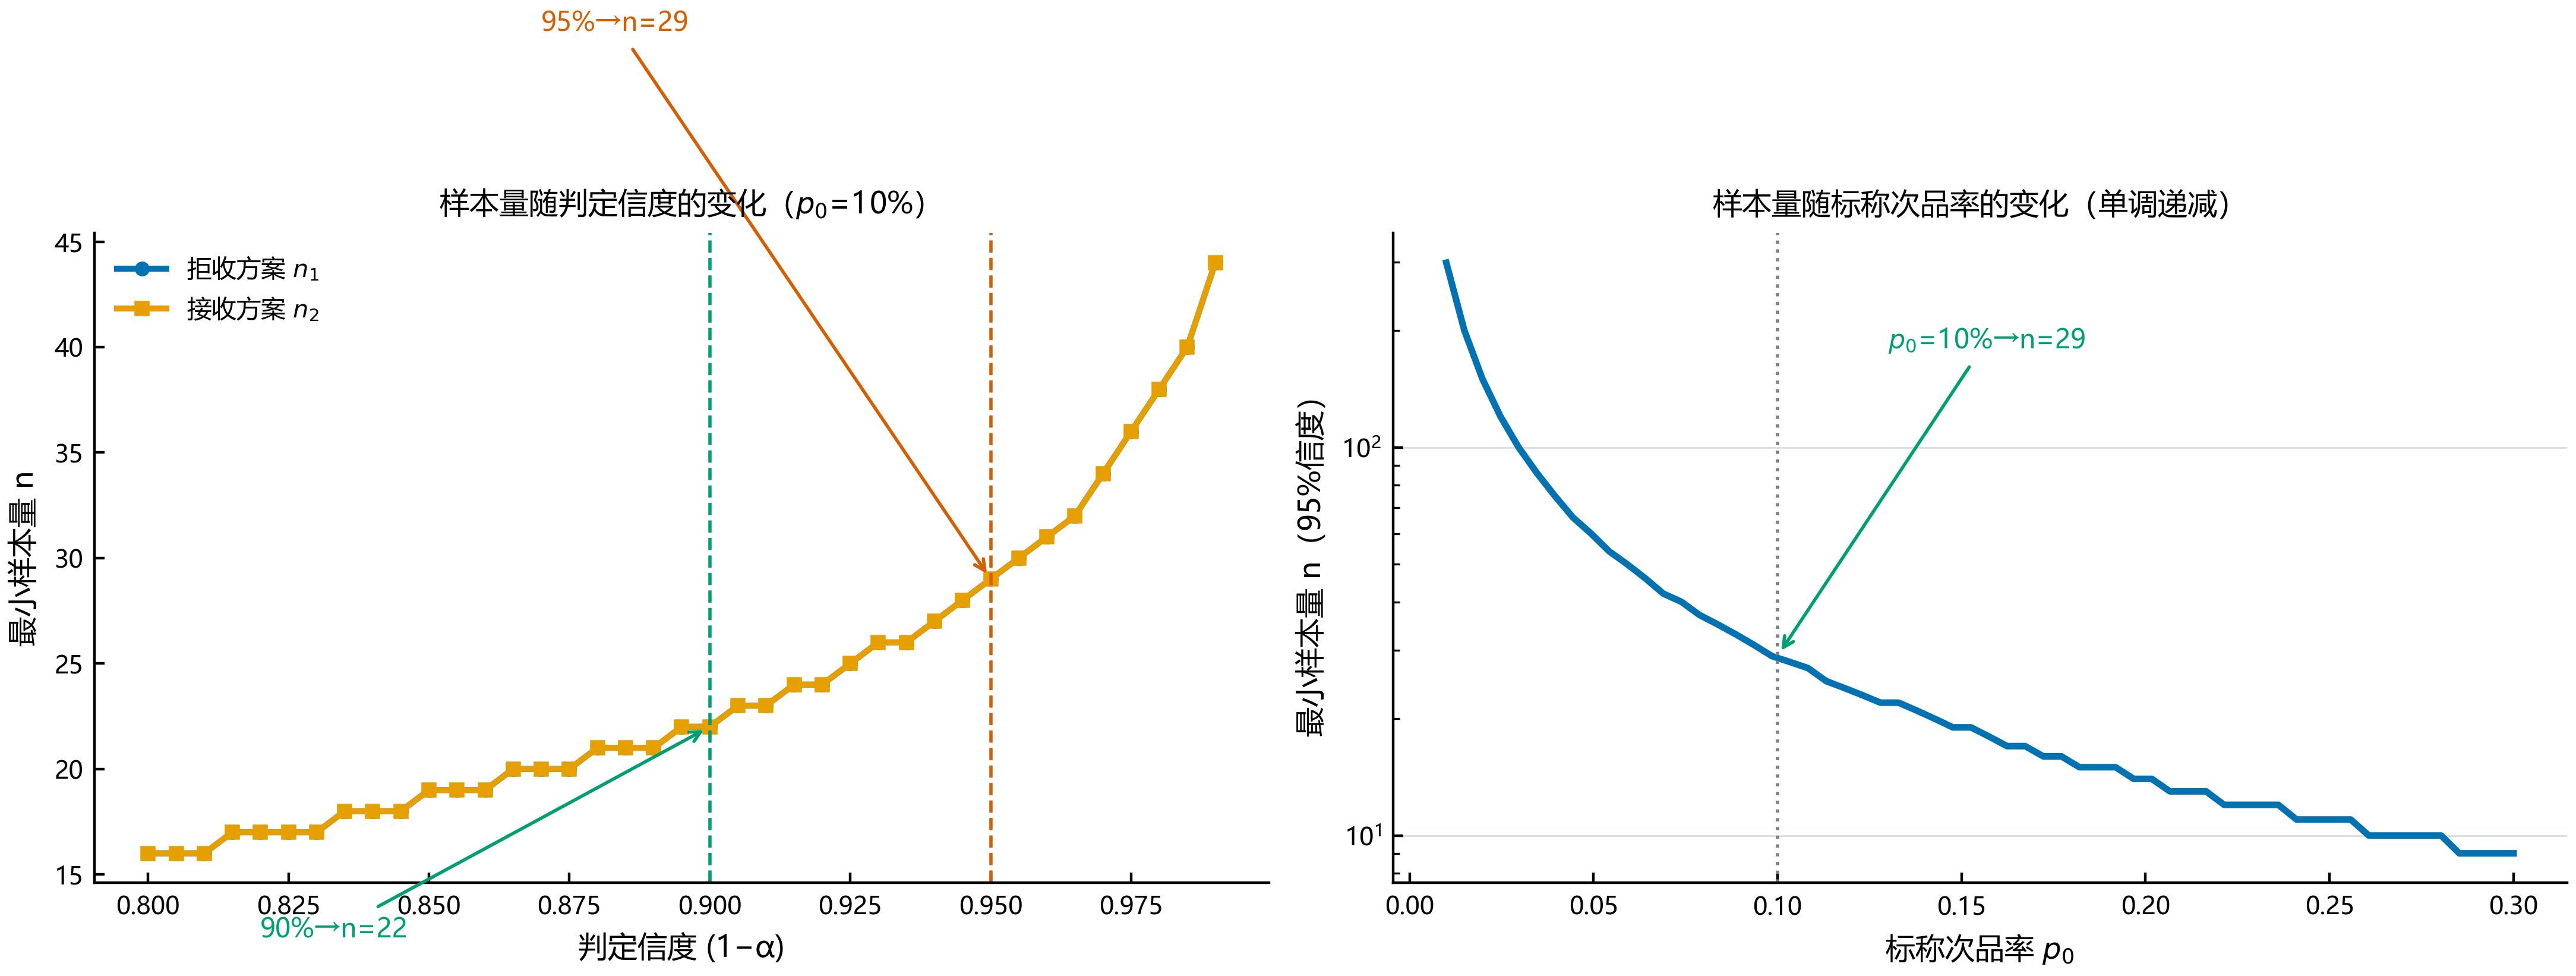
\includegraphics[width=0.85\textwidth]{fig5_confidence_sweep.png}
    \caption{最小样本量 $n$ 随信度 $c \in [0.80, 0.99]$ 的扫描。
    横轴为信度，纵轴为 $n$（$p_0 = 10\%$）。$c$ 从 0.80 升到 0.99
    时，$n$ 从 16 单调上升至 44；题设 90\%、95\% 两个工作点对应
    $n = 22$、$n = 29$ 恰为扫描曲线上的两个台阶点，与 §5.1.3
    闭式结果完全一致。}
    \label{fig:q1-confidence-sweep}
\end{figure}

扫描结果显示，$n$ 在 0.90--0.95 区间从 22 升至 29，0.99
处达 44，接近翻倍。高信度区间的样本量增长不能从 95\% 处
线性外推，从 95\% 提升到 99\% 的边际成本很高。

%% ---------- 问题二 ----------
\subsection{问题二的建模与求解}
\label{sec:q2}

\subsubsection{模型构建}

\textbf{1. 决策变量与策略编码}

问题 2 涉及 4 个 0-1 决策变量：

\begin{table}[htbp]
\centering
\small
\begin{tabular}{ccl}
\toprule[1.5pt]
\textbf{变量} & \textbf{含义} & \textbf{取 1 时的操作} \\
\midrule[1pt]
$x_1$ & 零配件 1 是否检测 & 检测并剔除次品 \\
$x_2$ & 零配件 2 是否检测 & 检测并剔除次品 \\
$x_3$ & 成品是否检测     & 不合格品不进入市场 \\
$x_4$ & 不合格成品是否拆解 & 拆解并回收零配件 \\
\bottomrule[1.5pt]
\end{tabular}
\end{table}

策略统一记为四元码 $x_1 x_2 x_3 x_4$，例如 $0011$ 表示不检测
两个零配件、检测成品并拆解不合格品。

\textbf{2. 统一核算口径}

题目要求对市场不合格品无条件调换，因此企业最终需要向客户
交付一件合格品。本文以"每服务一名客户"为统一核算单位：
当 $x_4 = 1$ 时不合格成品被拆解，回收件按原策略再处理，循环
直至得到合格品；当 $x_4 = 0$ 时不合格成品报废，重新采购并
生产，直至得到合格品。两类分支产出口径相同，利润可直接
比较。

\textbf{3. 质量传播}

进入装配的零配件 $i$ 的实际次品率为
\begin{equation}
    e_i = p_i (1 - x_i), \quad i = 1, 2.
\end{equation}
由于两个零配件均合格时仍可能因工艺 $p_0$ 出次品，成品的实际
不合格率为
\begin{equation}
    q = 1 - (1 - e_1)(1 - e_2)(1 - p_0).
    \label{eq:q2-q}
\end{equation}

\textbf{4. 首轮配件成本与回收件成本}

首轮期望配件成本
\begin{equation}
    C_{\mathrm{part}}
    = \sum_{i=1}^{2} \left[ (1 - x_i) c_i + x_i \frac{c_i + d_i}{1 - p_i} \right].
\end{equation}
回收件免采购，但若该零配件设置检测，仍需检测、剔除并补货：
\begin{equation}
    D = \sum_{i=1}^{2} x_i \frac{d_i + c_i p_i}{1 - p_i}.
\end{equation}
每轮基础加工成本 $B = a + x_3 d_0$。

\textbf{5. 两类处置分支的期望成本}

若拆解不合格成品（$x_4 = 1$），期望成本
\begin{equation}
    C(x \mid x_4 = 1) = C_{\mathrm{part}}
    + \frac{B + q (f + D)}{1 - q}.
\end{equation}
若不拆解（$x_4 = 0$），每次失败后整体重购：
\begin{equation}
    C(x \mid x_4 = 0) = \frac{C_{\mathrm{part}} + B}{1 - q}.
\end{equation}

\textbf{6. 期望收入与目标函数}

期望收入
\begin{equation}
    R(x) =
    \begin{cases}
        s, & x_3 = 1, \\[2mm]
        s - \dfrac{q r}{1 - q}, & x_3 = 0.
    \end{cases}
\end{equation}
最终目标为
\begin{equation}
    \max_{x \in \{0,1\}^4} \pi(x) = R(x) - C(x).
    \label{eq:q2-opt}
\end{equation}

\subsubsection{求解方法}

由于决策空间仅有 $2^4 = 16$ 个元素，直接全枚举比连续松弛
或启发式搜索更可靠：无初值依赖、无局部最优陷阱、结果可严格
复核。每种情形均保存全部 16 种策略的利润，并用 20 万次蒙特卡洛
逐件模拟作独立验证。

\begin{figure}[htbp]
    \centering
    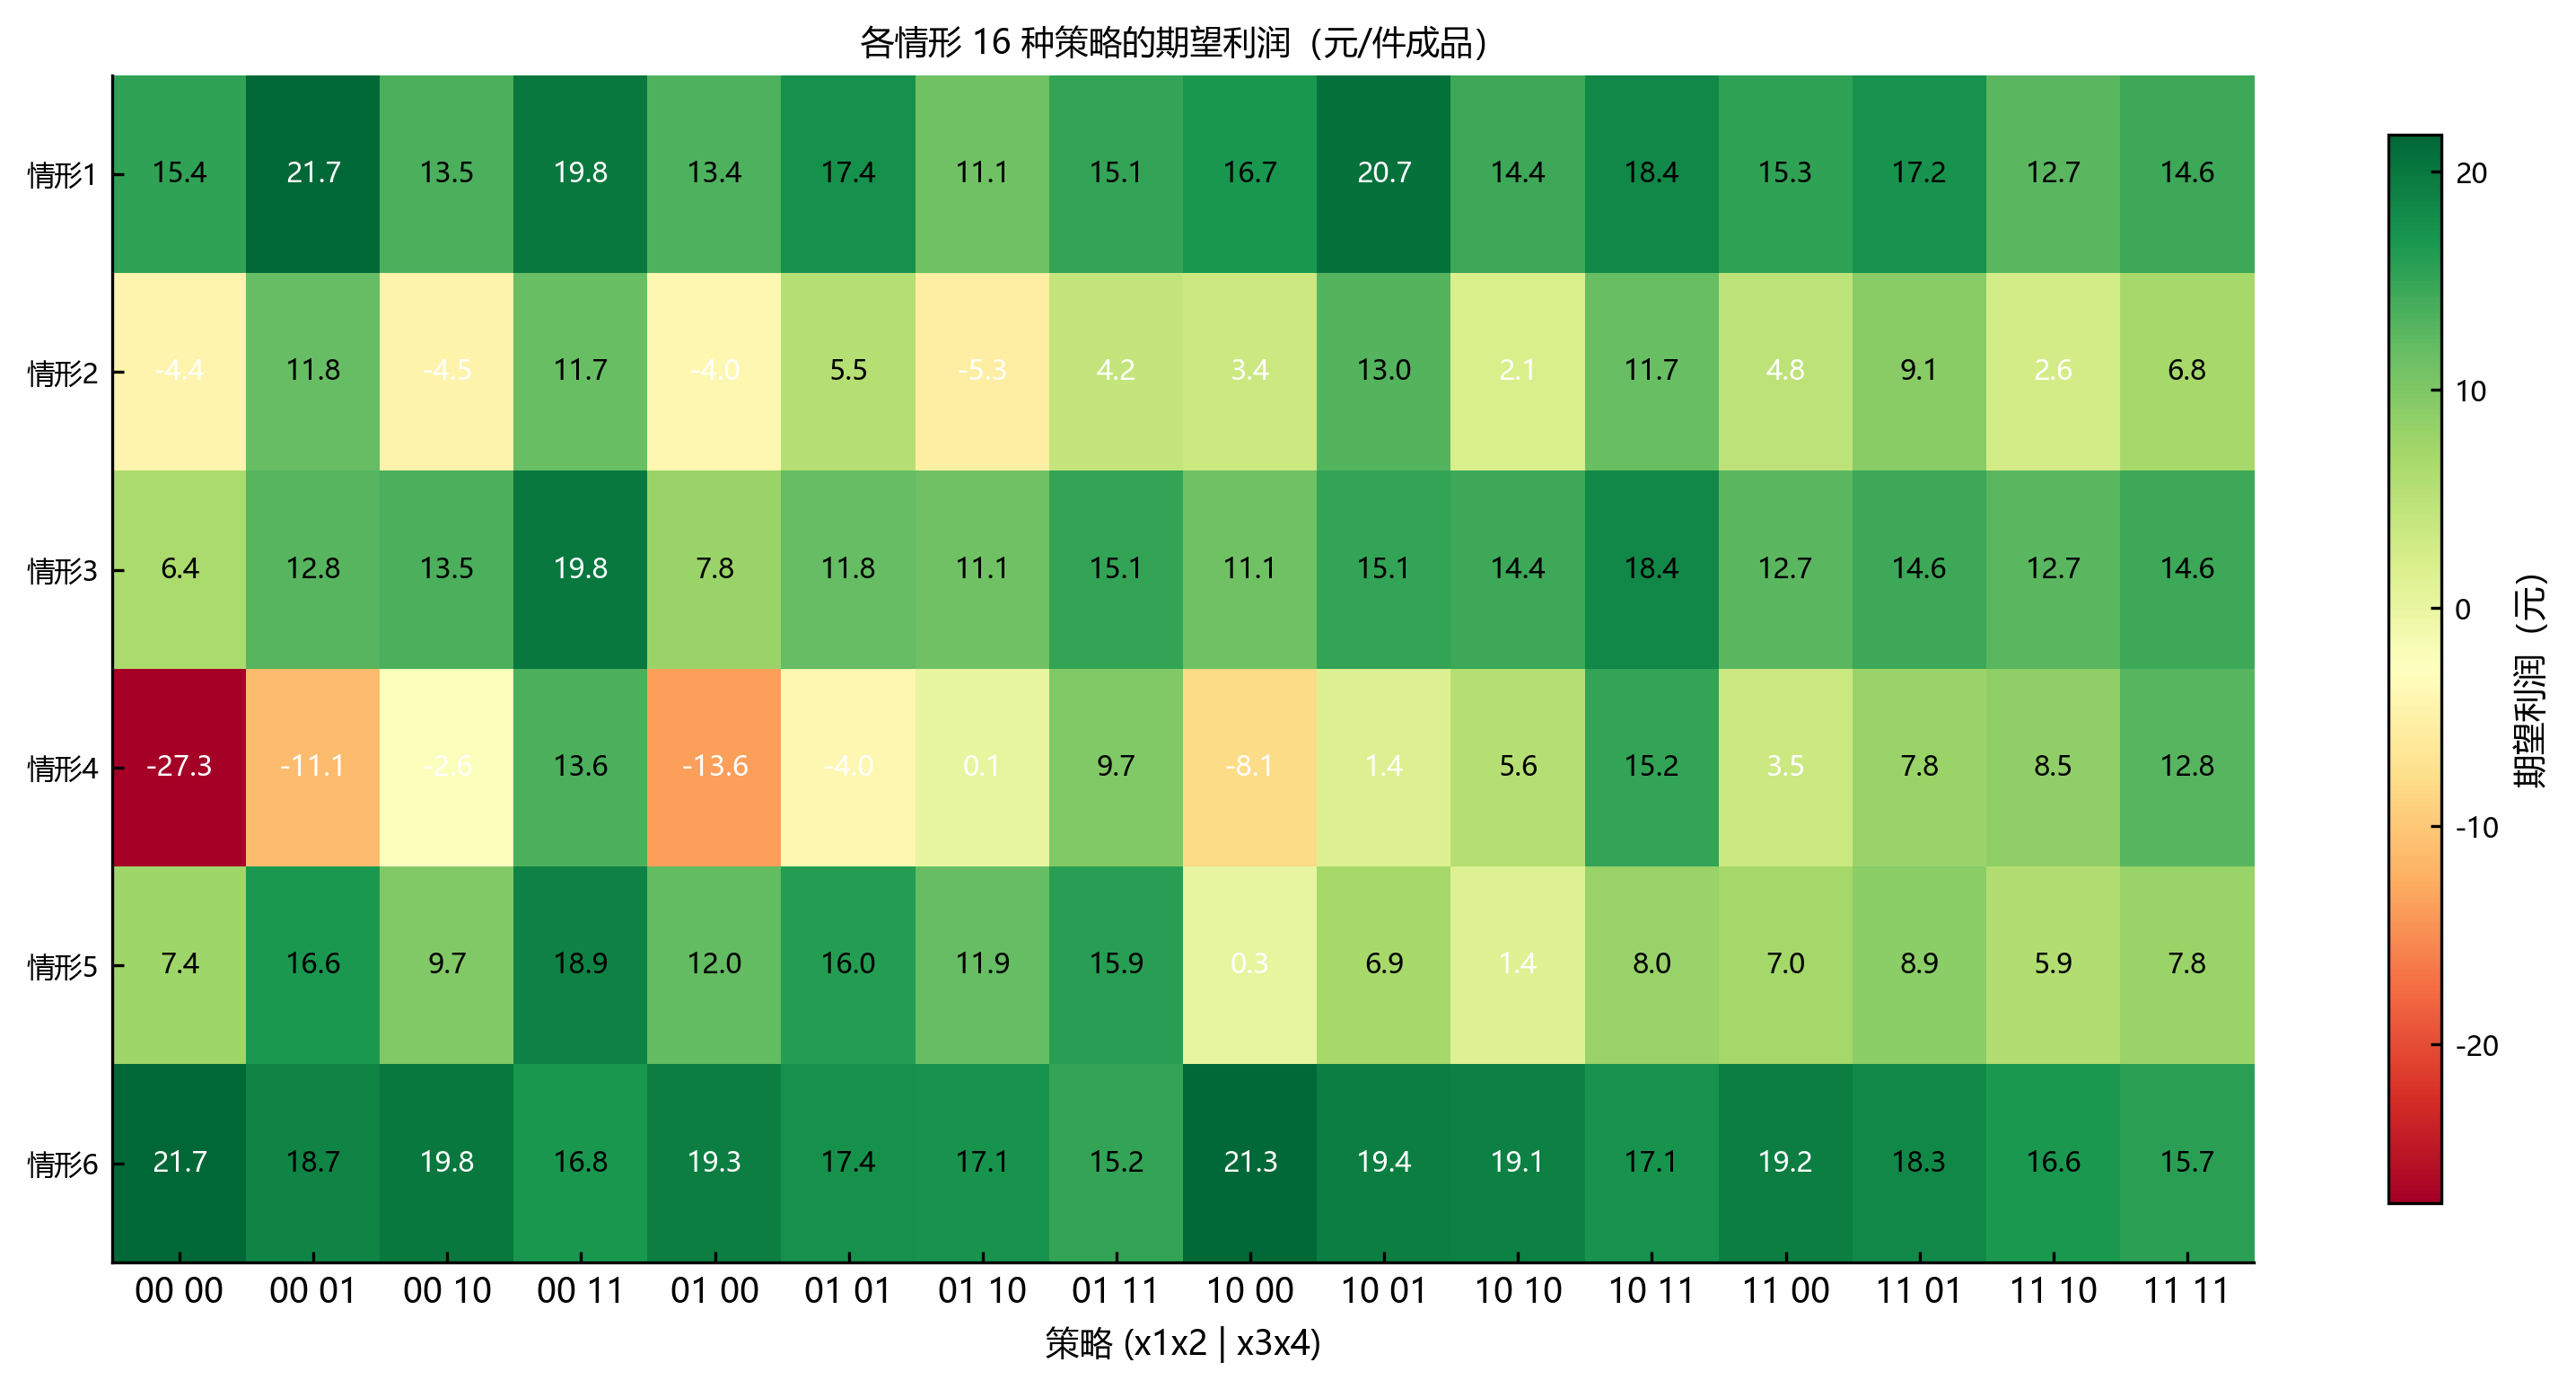
\includegraphics[width=0.92\textwidth]{fig1_strategy_heatmap.png}
    \caption{16 种检测策略 $\texttt{x}_1\texttt{x}_2\texttt{|}\texttt{x}_3\texttt{x}_4$
    在 6 种情形下的期望利润热图（颜色越深红利润越高，蓝色框标记每种情形下的
    最优策略）。全枚举共 $2^4 = 16$ 个候选，单次评估常数代价极低，
    因此本文直接以全枚举代替启发式搜索，保证最优性可严格复核。}
    \label{fig:q2-strategy-heatmap}
\end{figure}

\subsubsection{结果分析}

\textbf{1. 六种情形最优策略}

表 \ref{tab:q2-result} 给出 6 种情形下的全局最优策略及关键
指标。

\begin{table}[htbp]
\centering
\caption{问题 2 六种情形下的全局最优策略及关键指标}
\label{tab:q2-result}
\small
\begin{tabular}{cccccc}
\toprule[1.5pt]
情形 & 最优策略 & $q$ & 期望收入（元/件） & 期望总成本（元/件） & 期望利润（元/件） \\
\midrule[1pt]
1 & \texttt{0001} & 0.2710 & 53.7695 & 32.0891 & \textbf{21.6804} \\
2 & \texttt{1001} & 0.3600 & 52.6250 & 39.6562 & \textbf{12.9688} \\
3 & \texttt{0011} & 0.2710 & 56.0000 & 36.2044 & \textbf{19.7956} \\
4 & \texttt{1011} & 0.3600 & 56.0000 & 40.8281 & \textbf{15.1719} \\
5 & \texttt{0011} & 0.3520 & 56.0000 & 37.0617 & \textbf{18.9383} \\
6 & \texttt{0000} & 0.1426 & 54.3365 & 32.6578 & \textbf{21.6787} \\
\bottomrule[1.5pt]
\end{tabular}
\end{table}

\textbf{2. 决策规律}

由表 \ref{tab:q2-result} 与模型参数可归纳以下四条决策规律：

\begin{enumerate}
    \item \textbf{零配件 2 在六种情形中均不检测}。其采购价高
    （18 元/件），为获得一件合格配件而重复购入的期望成本
    较大，下游统一处理更经济。
    \item \textbf{零配件 1 仅在情形 2、4 检测}。这两种情形
    零配件次品率较高（20\%），且情形 4 检测费低（1 元/件），
    前端拦截的边际收益超过检测成本。
    \item \textbf{成品检测由调换损失与检测费共同驱动}。
    情形 3、4、5 因调换损失高（$r = 30$ 或 $r = 10$）开启
    成品检测，避免高额市场退换损失。
    \item \textbf{拆解决策受拆解费支配}。情形 1--5 拆解费
    $f = 5$，回收价值超过拆解成本；情形 6 中 $f = 40$ 过高，
    最优策略转为 \texttt{0000}，整体重购更经济。
\end{enumerate}

\subsubsection{模型检验}

\textbf{1. 蒙特卡洛验证}

为检验解析模型的数值正确性，对 6 种情形分别用 20 万次蒙特卡洛
逐件模拟比较。六情形下解析最优与模拟最优的相对误差范围为
$0.04\% \sim 1.25\%$，且不存在系统性高估或低估。误差来源
主要为有限模拟样本，随模拟次数 $M$ 增大以 $O(1/\sqrt{M})$
收敛。

\begin{figure}[htbp]
    \centering
    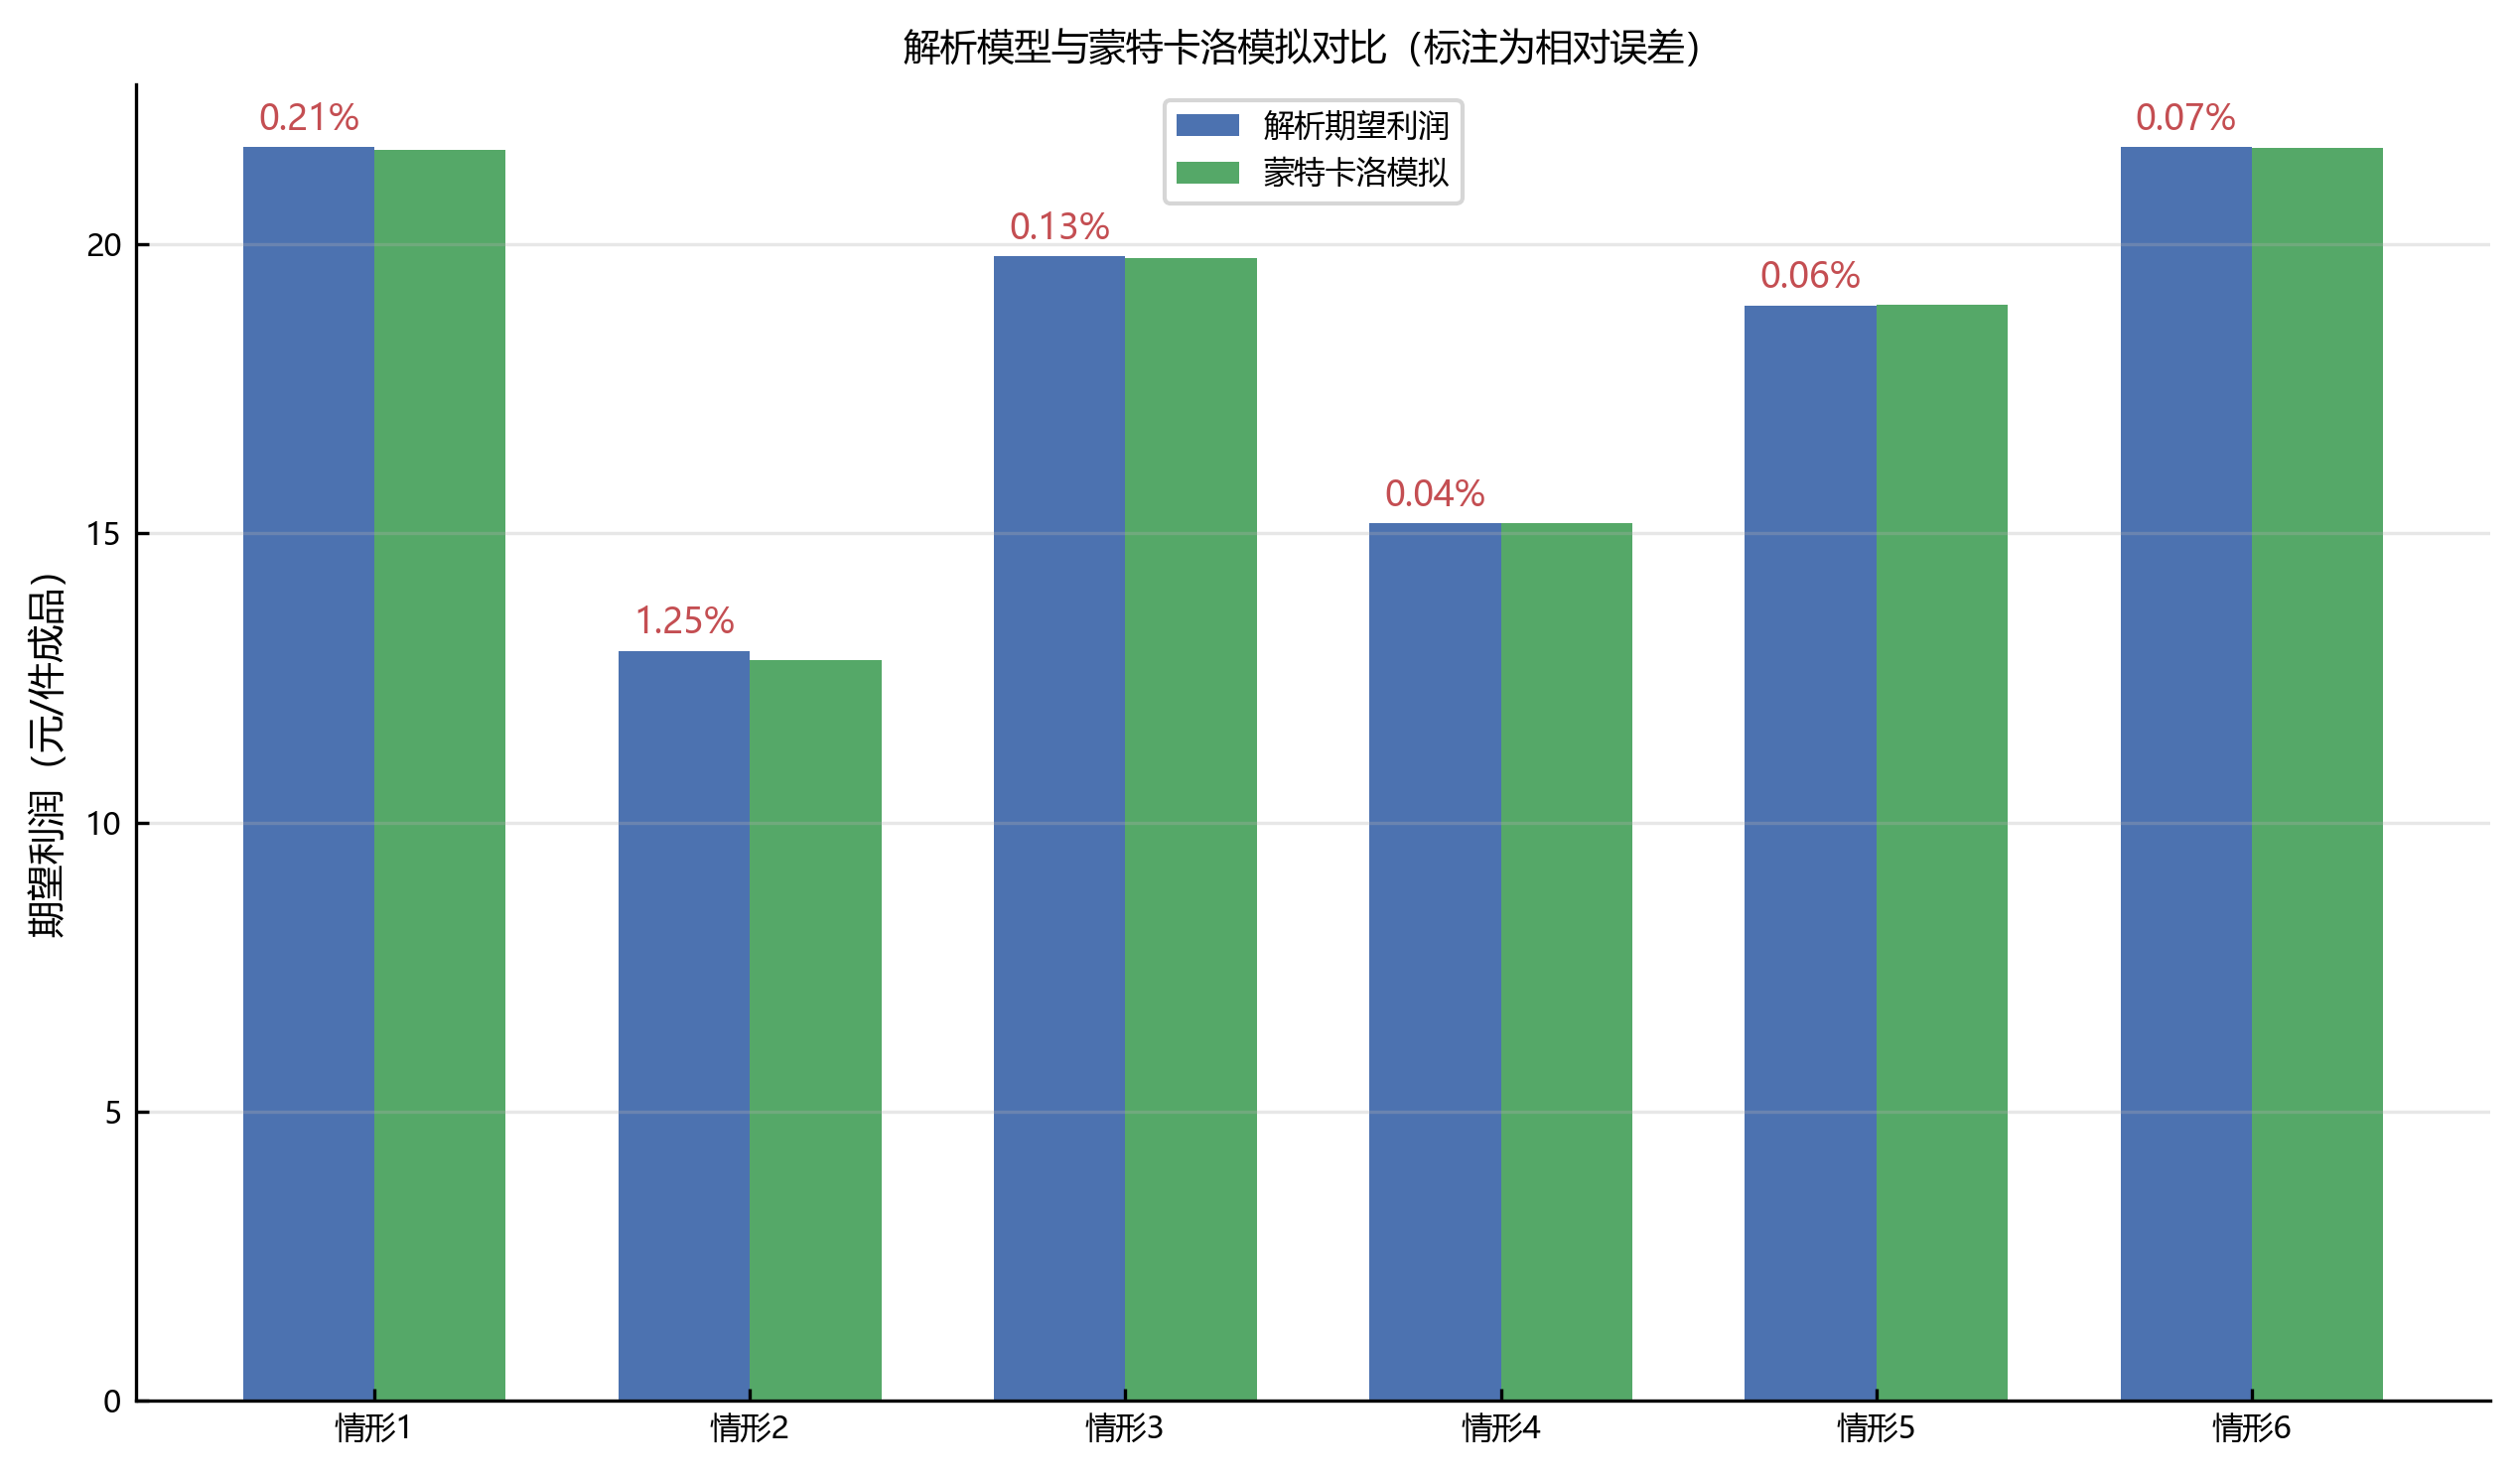
\includegraphics[width=0.92\textwidth]{fig3_analytic_vs_sim.png}
    \caption{解析模型与蒙特卡洛模拟（$M = 20$ 万次）所得最优利润的对照。
    蓝点为解析值，方块为模拟值，连线长度表征二者差距，文本标注相对误差。
    各情形相对误差均在 $0.04\% \sim 1.25\%$ 之间，且不存在系统性高估或
    低估，验证了解析推导的正确性。}
    \label{fig:q2-analytic-sim}
\end{figure}

\textbf{2. 单参数分岔}

以情形 1 为基线进行单变量扫描，得到以下关键翻转点：
\begin{itemize}
    \item 零配件 1 检测费 $1.25 \to 1.50$ 时，策略由 \texttt{1001}
    转为 \texttt{0001}；
    \item 调换损失 $10 \to 12$ 时，策略由 \texttt{0001} 转为
    \texttt{0011}；
    \item 拆解费 $12 \to 13$ 时，策略由 \texttt{0001} 转为
    \texttt{1001}；
    \item 零配件 2 检测费与市场售价在给定扫描范围内未引发翻转。
\end{itemize}
这组结果说明模型具有符合业务逻辑的阈值响应，而非数值偶然。

\begin{figure}[htbp]
    \centering
    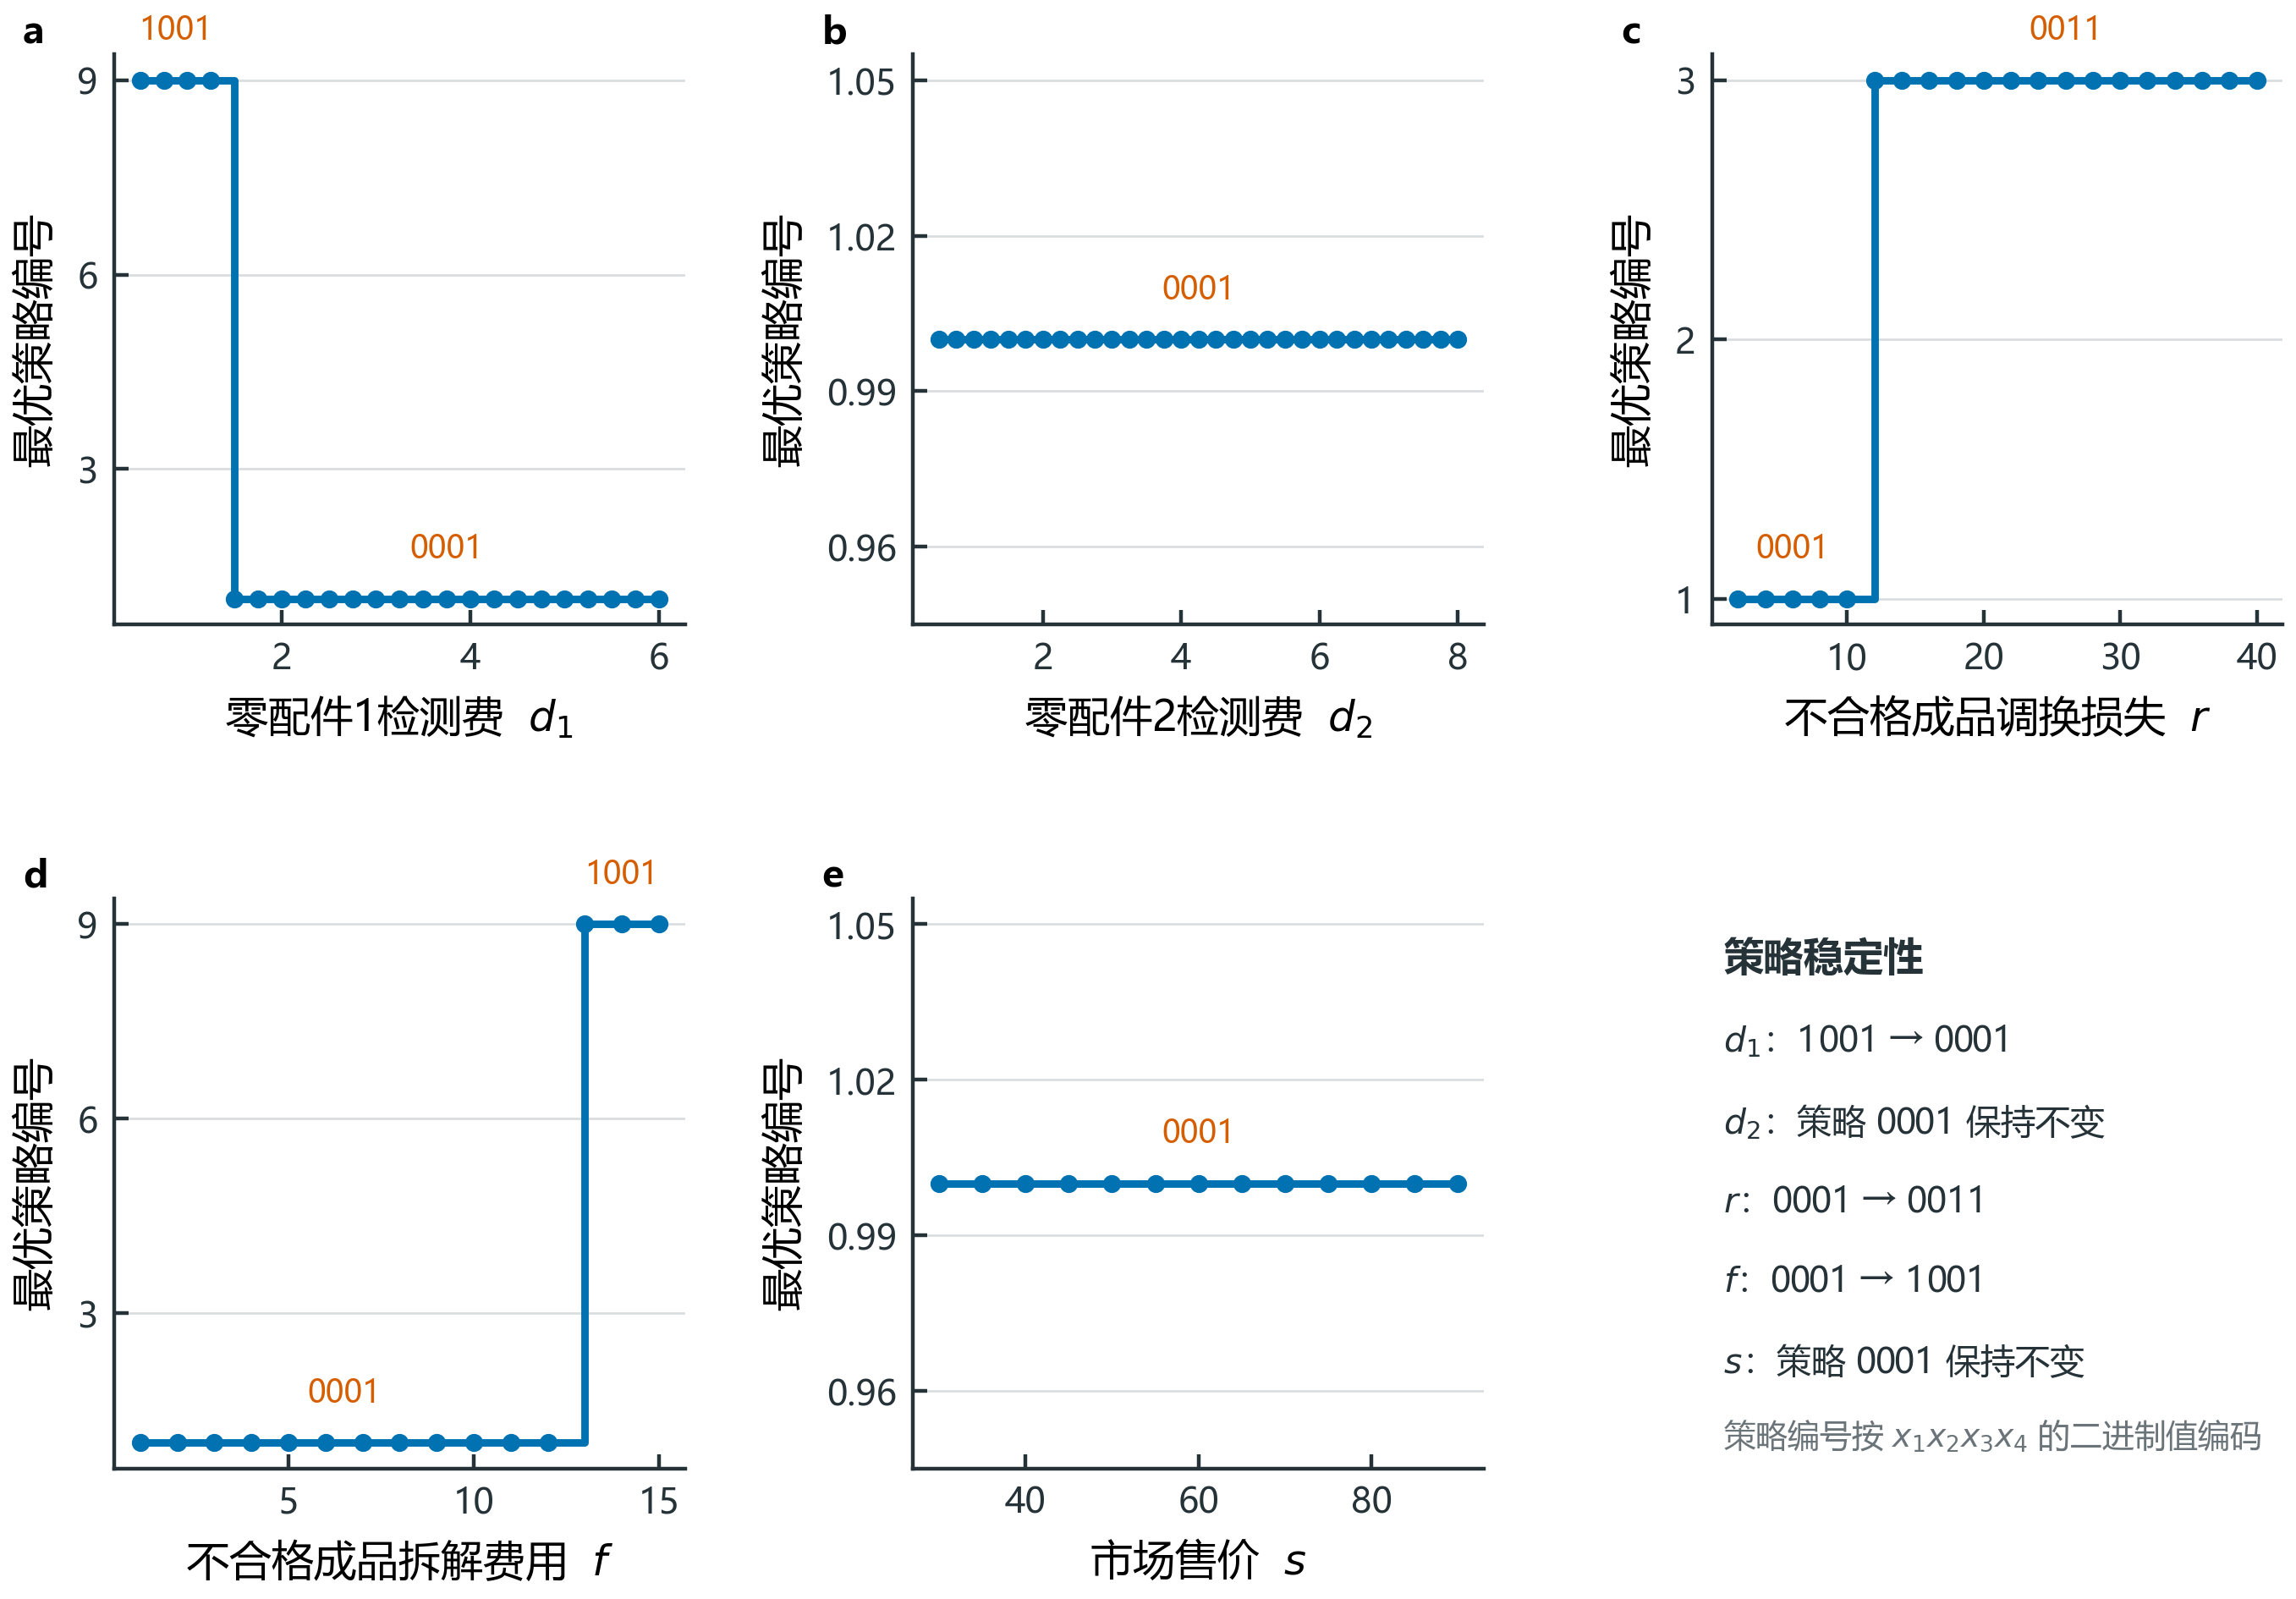
\includegraphics[width=0.95\textwidth]{fig4_decision_bifurcation.png}
    \caption{情形 1 为基线的单参数分岔图。每个子图横轴扫描一个经济
    参数（检测费、装配费、调换损失等），纵轴为最优策略编码
    $\texttt{x}_1\texttt{x}_2\texttt{x}_3\texttt{x}_4$。竖虚线标注
    关键翻转点：配件 1 检测费 $1.25 \to 1.50$ 时由 \texttt{1001}
    转为 \texttt{0001}；调换损失 $10 \to 12$ 时由 \texttt{0001}
    转为 \texttt{0011}；拆解费 $12 \to 13$ 时由 \texttt{0001}
    转为 \texttt{1001}。翻转点与正文一致。}
    \label{fig:q2-bifurcation}
\end{figure}

\textbf{3. 跨情形最小最大遗憾}

若决策者事前不知道将处于哪种情形，而必须预先固定一个统一
策略，可定义遗憾 $R_{ks} = \pi_k^\star - \pi_{ks}$。对 16 种
策略的遗憾进行统计，策略 \texttt{0011} 的平均遗憾仅 1.60 元/件、
最大遗憾 4.83 元/件，为 16 种策略中的最小最大遗憾方案。

\begin{figure}[htbp]
    \centering
    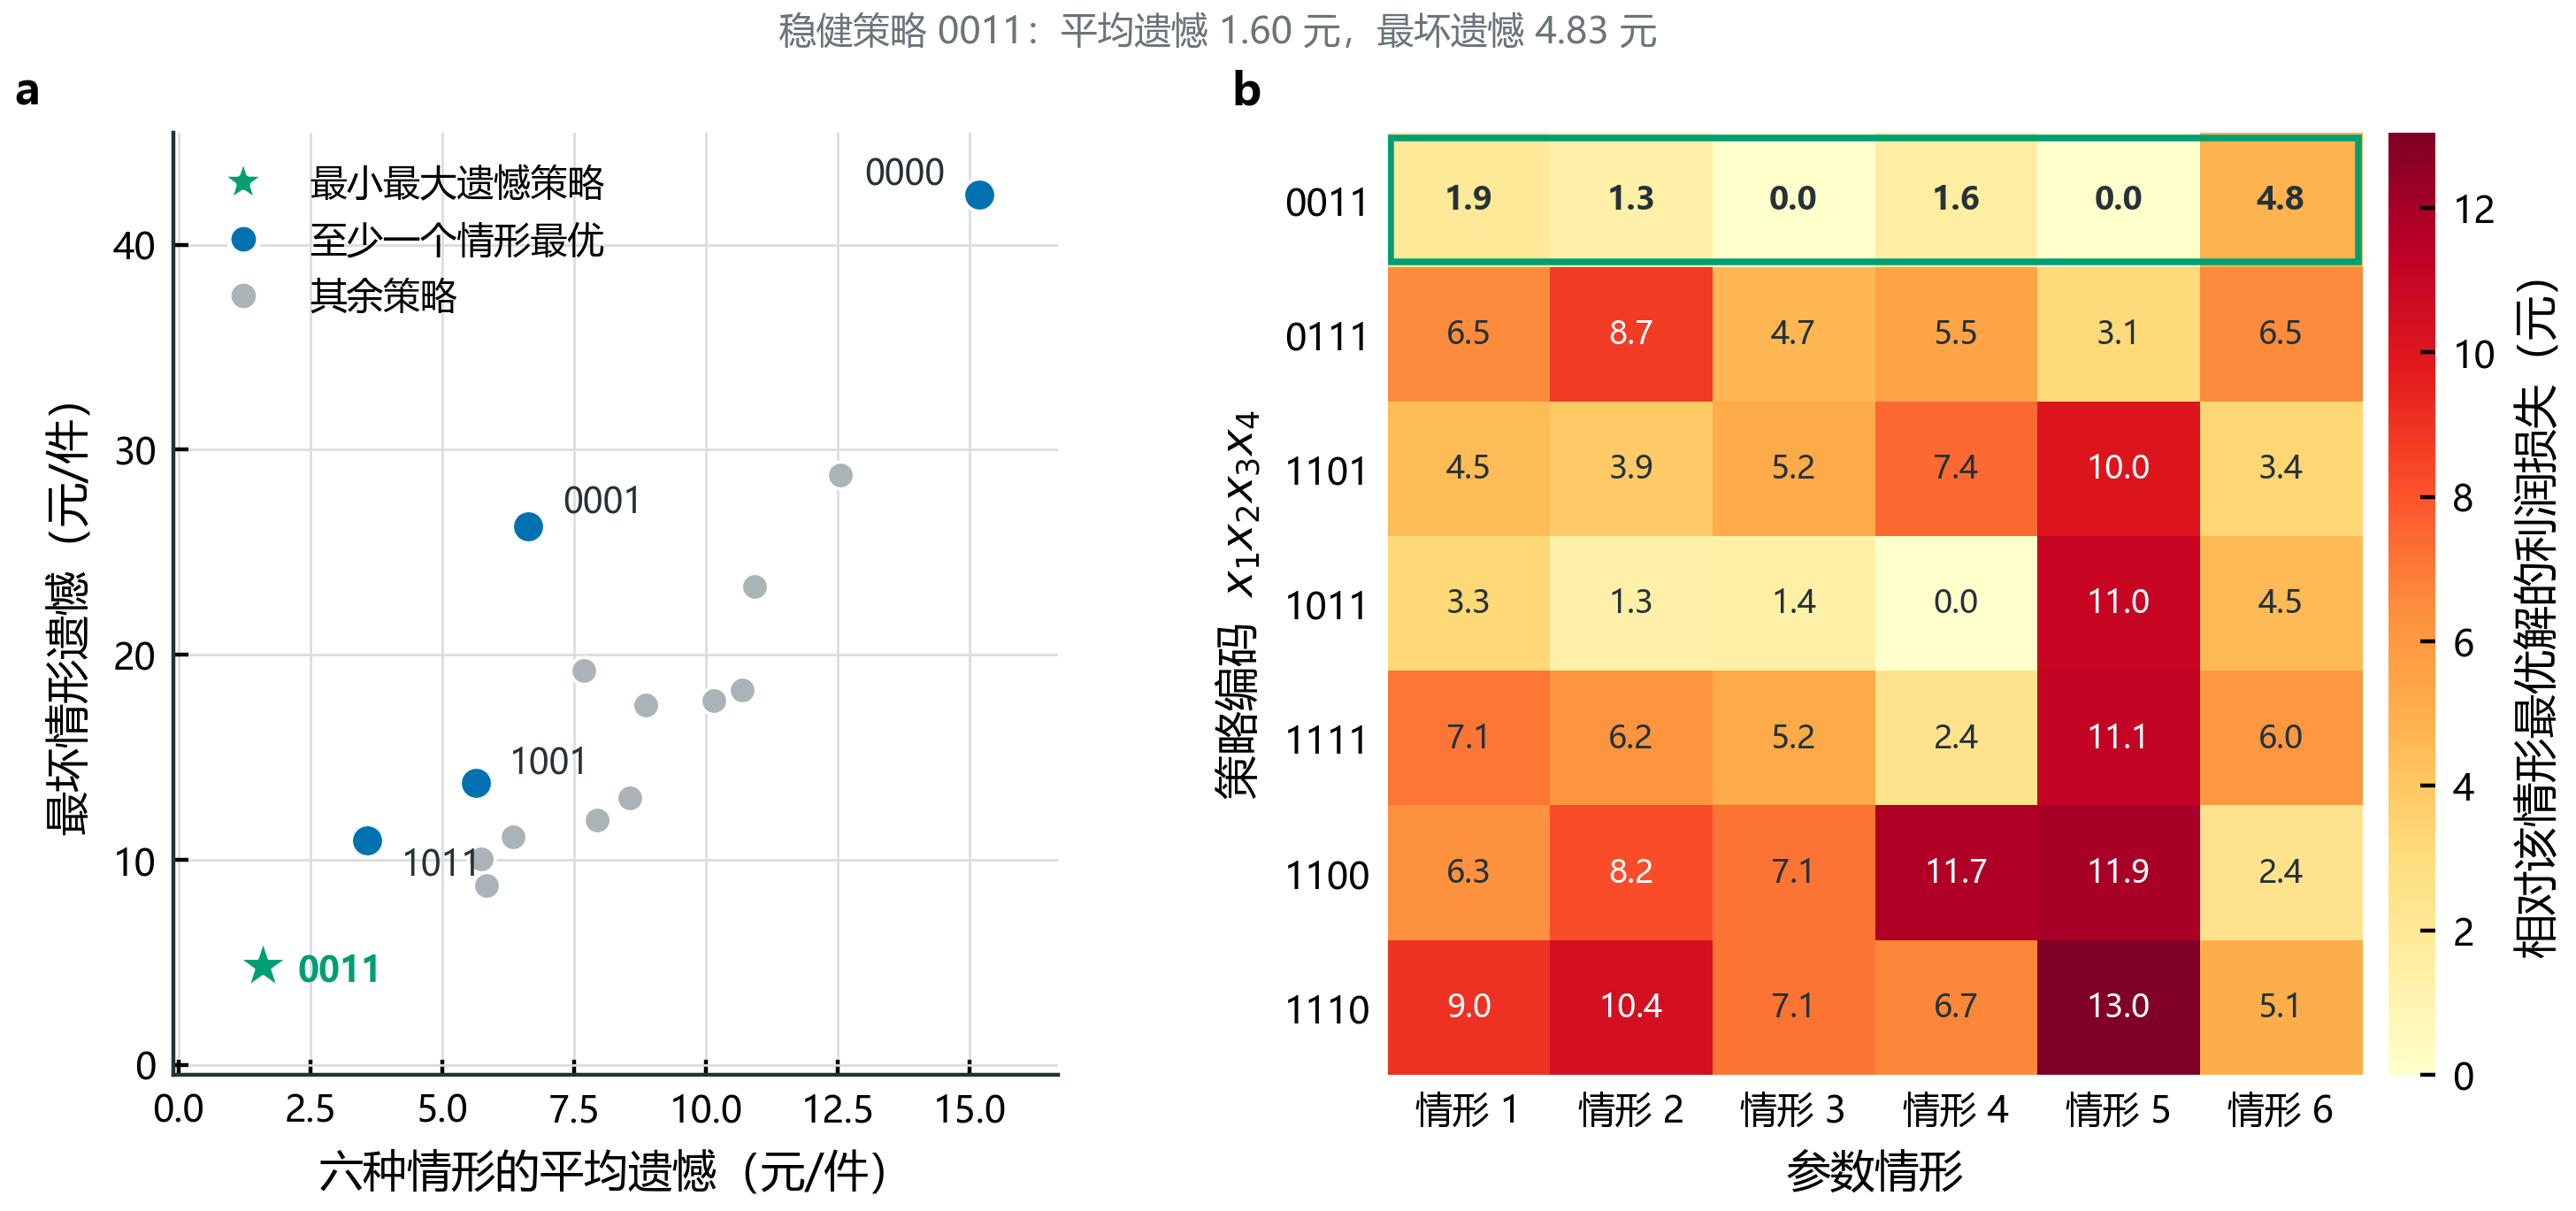
\includegraphics[width=0.95\textwidth]{fig_strategy_regret.png}
    \caption{16 种策略的跨情形遗憾分布。
    \textbf{(a)} 平均遗憾 vs 最大遗憾散点图，绿色星标为稳健策略
    \texttt{0011}，蓝色圆点为至少在一种情形最优的策略，灰色为其他。
    \textbf{(b)} 前 7 候选策略的跨情形遗憾热图，颜色越深表示遗憾越大。
    \texttt{0011} 的平均遗憾 1.60 元/件、最大遗憾 4.83 元/件，
    是 16 策略中的最小最大遗憾方案。}
    \label{fig:q2-regret}
\end{figure}

该结论不是说 \texttt{0011} 在每个情形都最优，而是说它在情形
未知时最不容易遭受严重后悔损失，是合理的稳健统一策略。

\textbf{4. 参数空间策略分布}

在六种情形邻域内抽取 8000 组参数并逐组全枚举：\texttt{0011}
出现频率最高（占 29.6\%）；$(x_1, x_2, x_3, x_4)$ 的边际
采用率分别为 46.6\%、29.3\%、68.0\%、66.5\%，表明成品检测
和拆解更常见，质量控制倾向集中于价值更高的下游节点。

\begin{figure}[htbp]
    \centering
    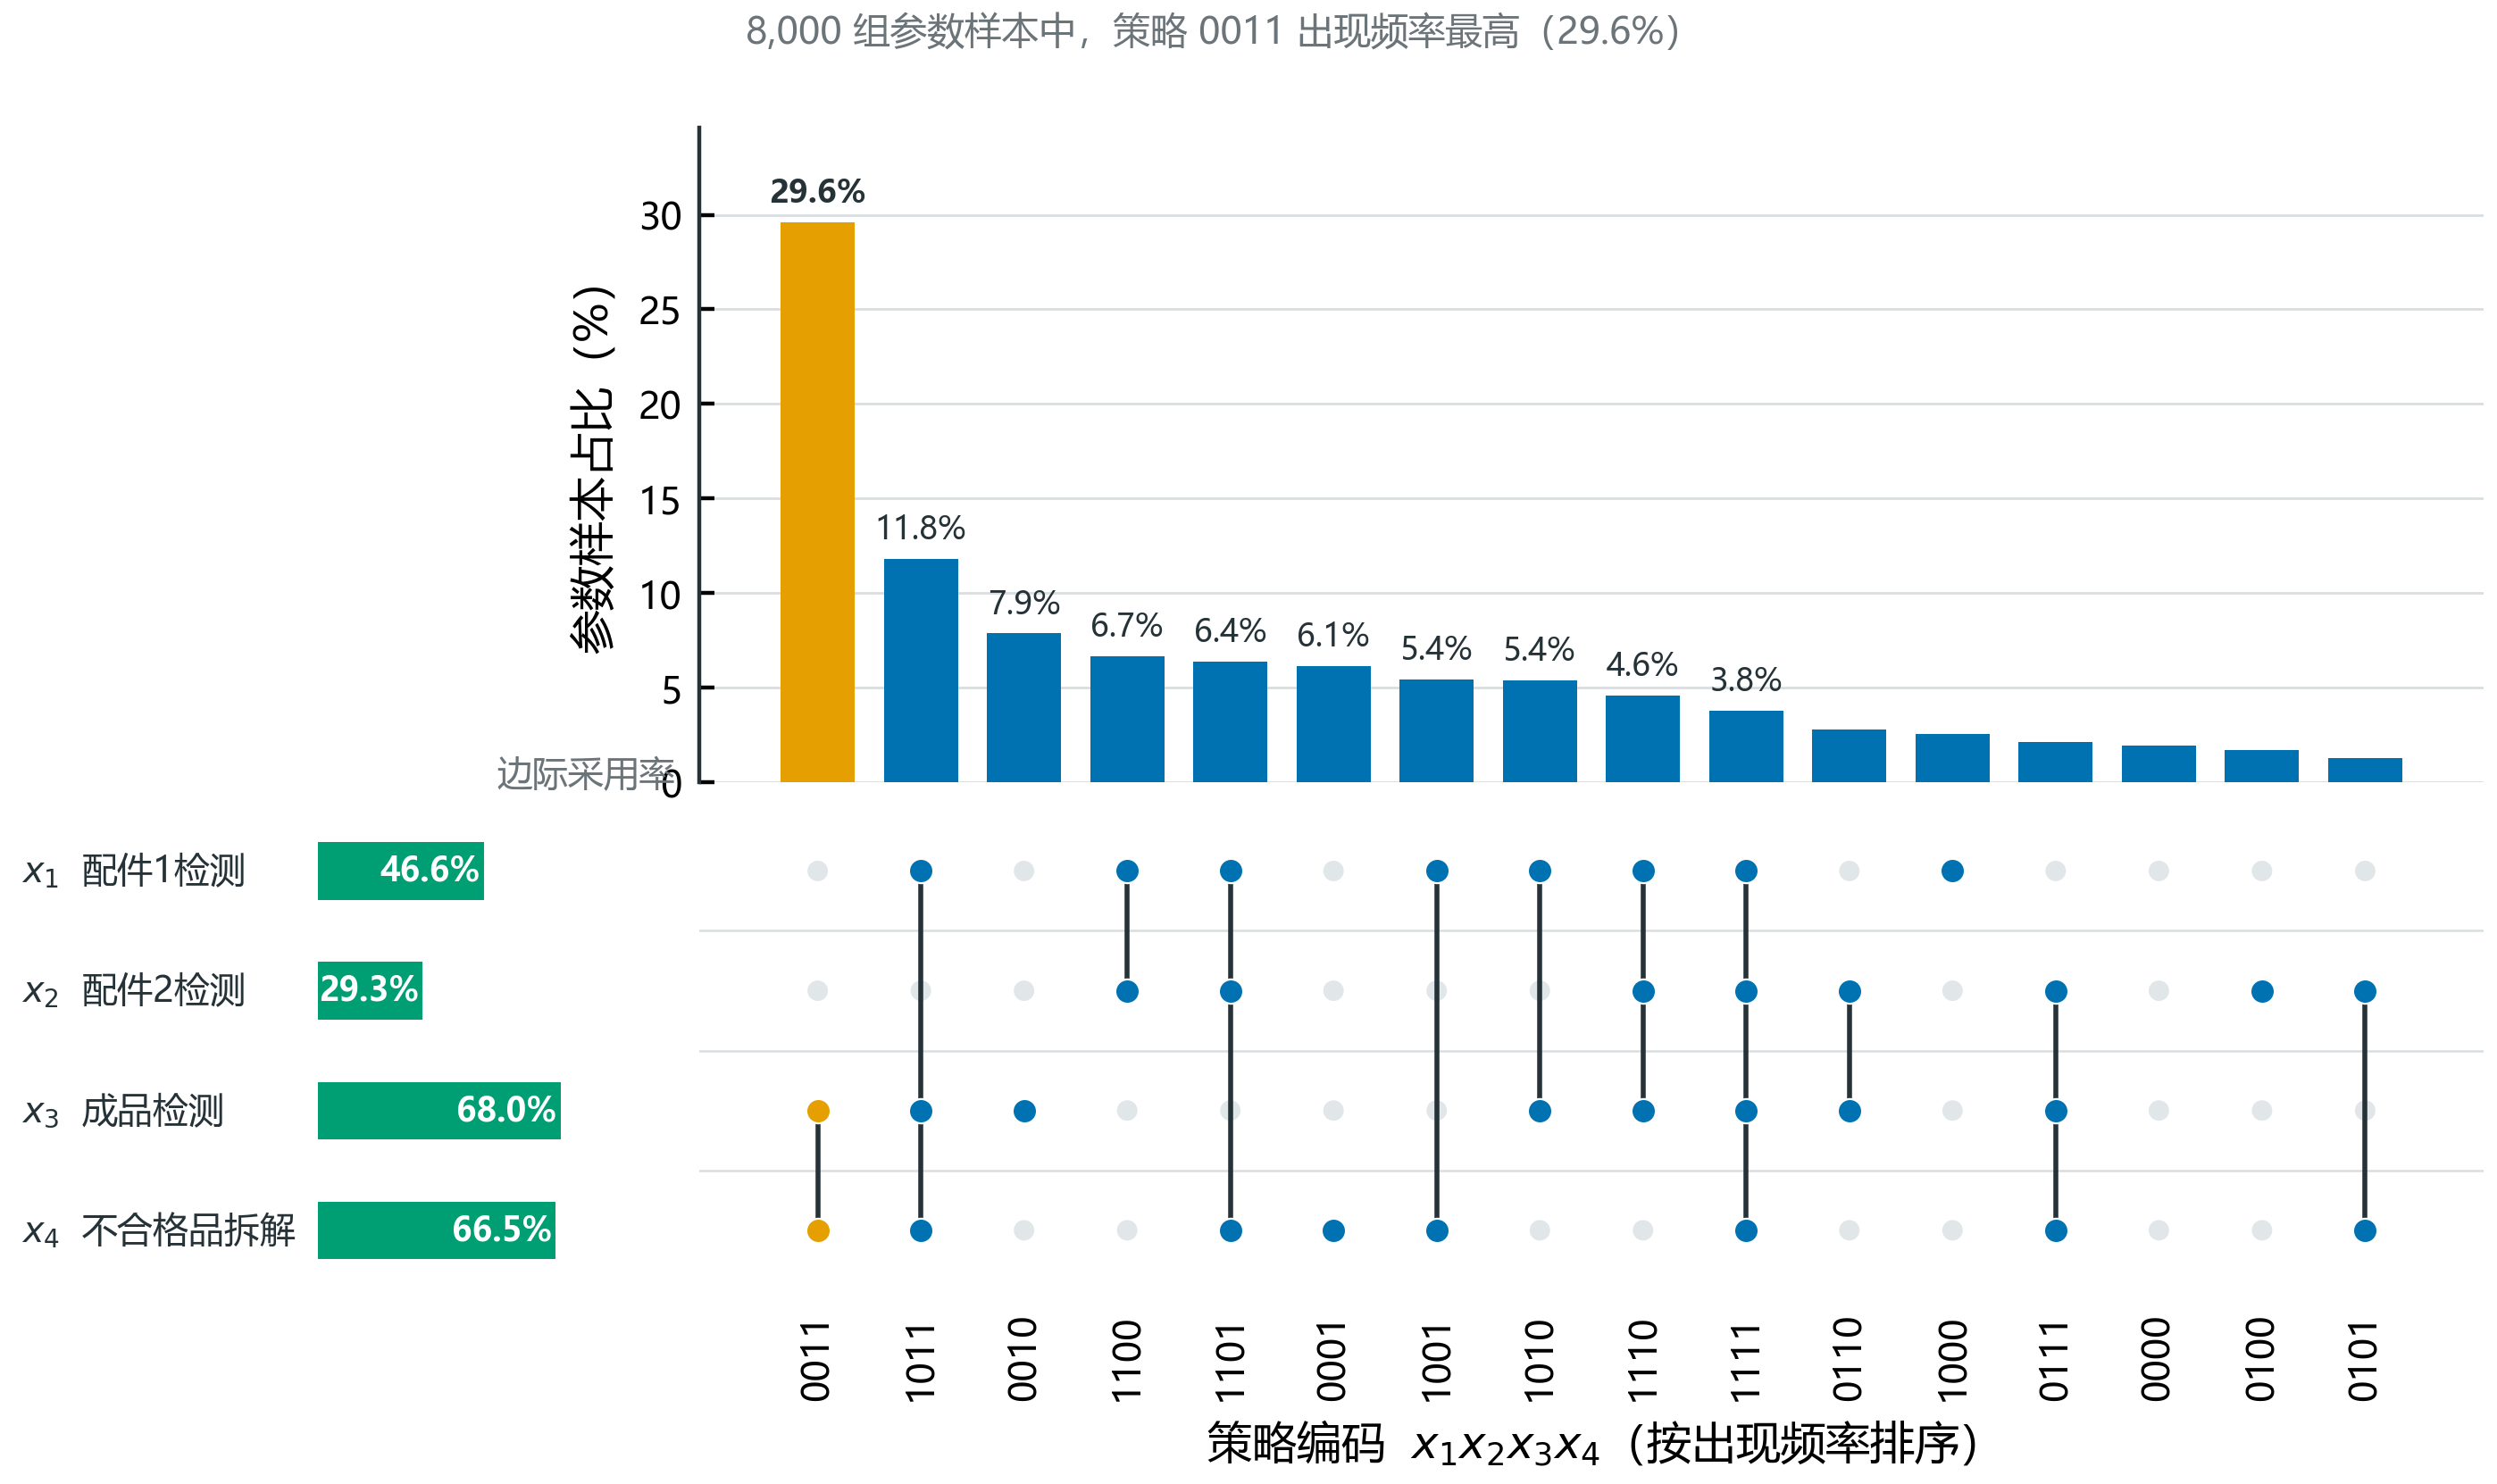
\includegraphics[width=0.95\textwidth]{fig_strategy_upset.png}
    \caption{8000 组参数下 16 种策略的出现频次与各决策的边际
    采用率。\texttt{0011} 出现频率最高（29.6\%），其次为
    \texttt{0000} 与 \texttt{0001}；右下角决策热图给出各
    决策变量的边际采用率：$x_1$ 46.6\%、$x_2$ 29.3\%、
    $x_3$ 68.0\%、$x_4$ 66.5\%，质量控制明显向价值更高的
    下游节点集中。}
    \label{fig:q2-upset}
\end{figure}

%% ---------- 问题三 ----------
\subsection{问题三的建模与求解}
\label{sec:q3}

\subsubsection{模型构建}

\textbf{1. 装配网络与决策变量}

\begin{figure}[htbp]
    \centering
    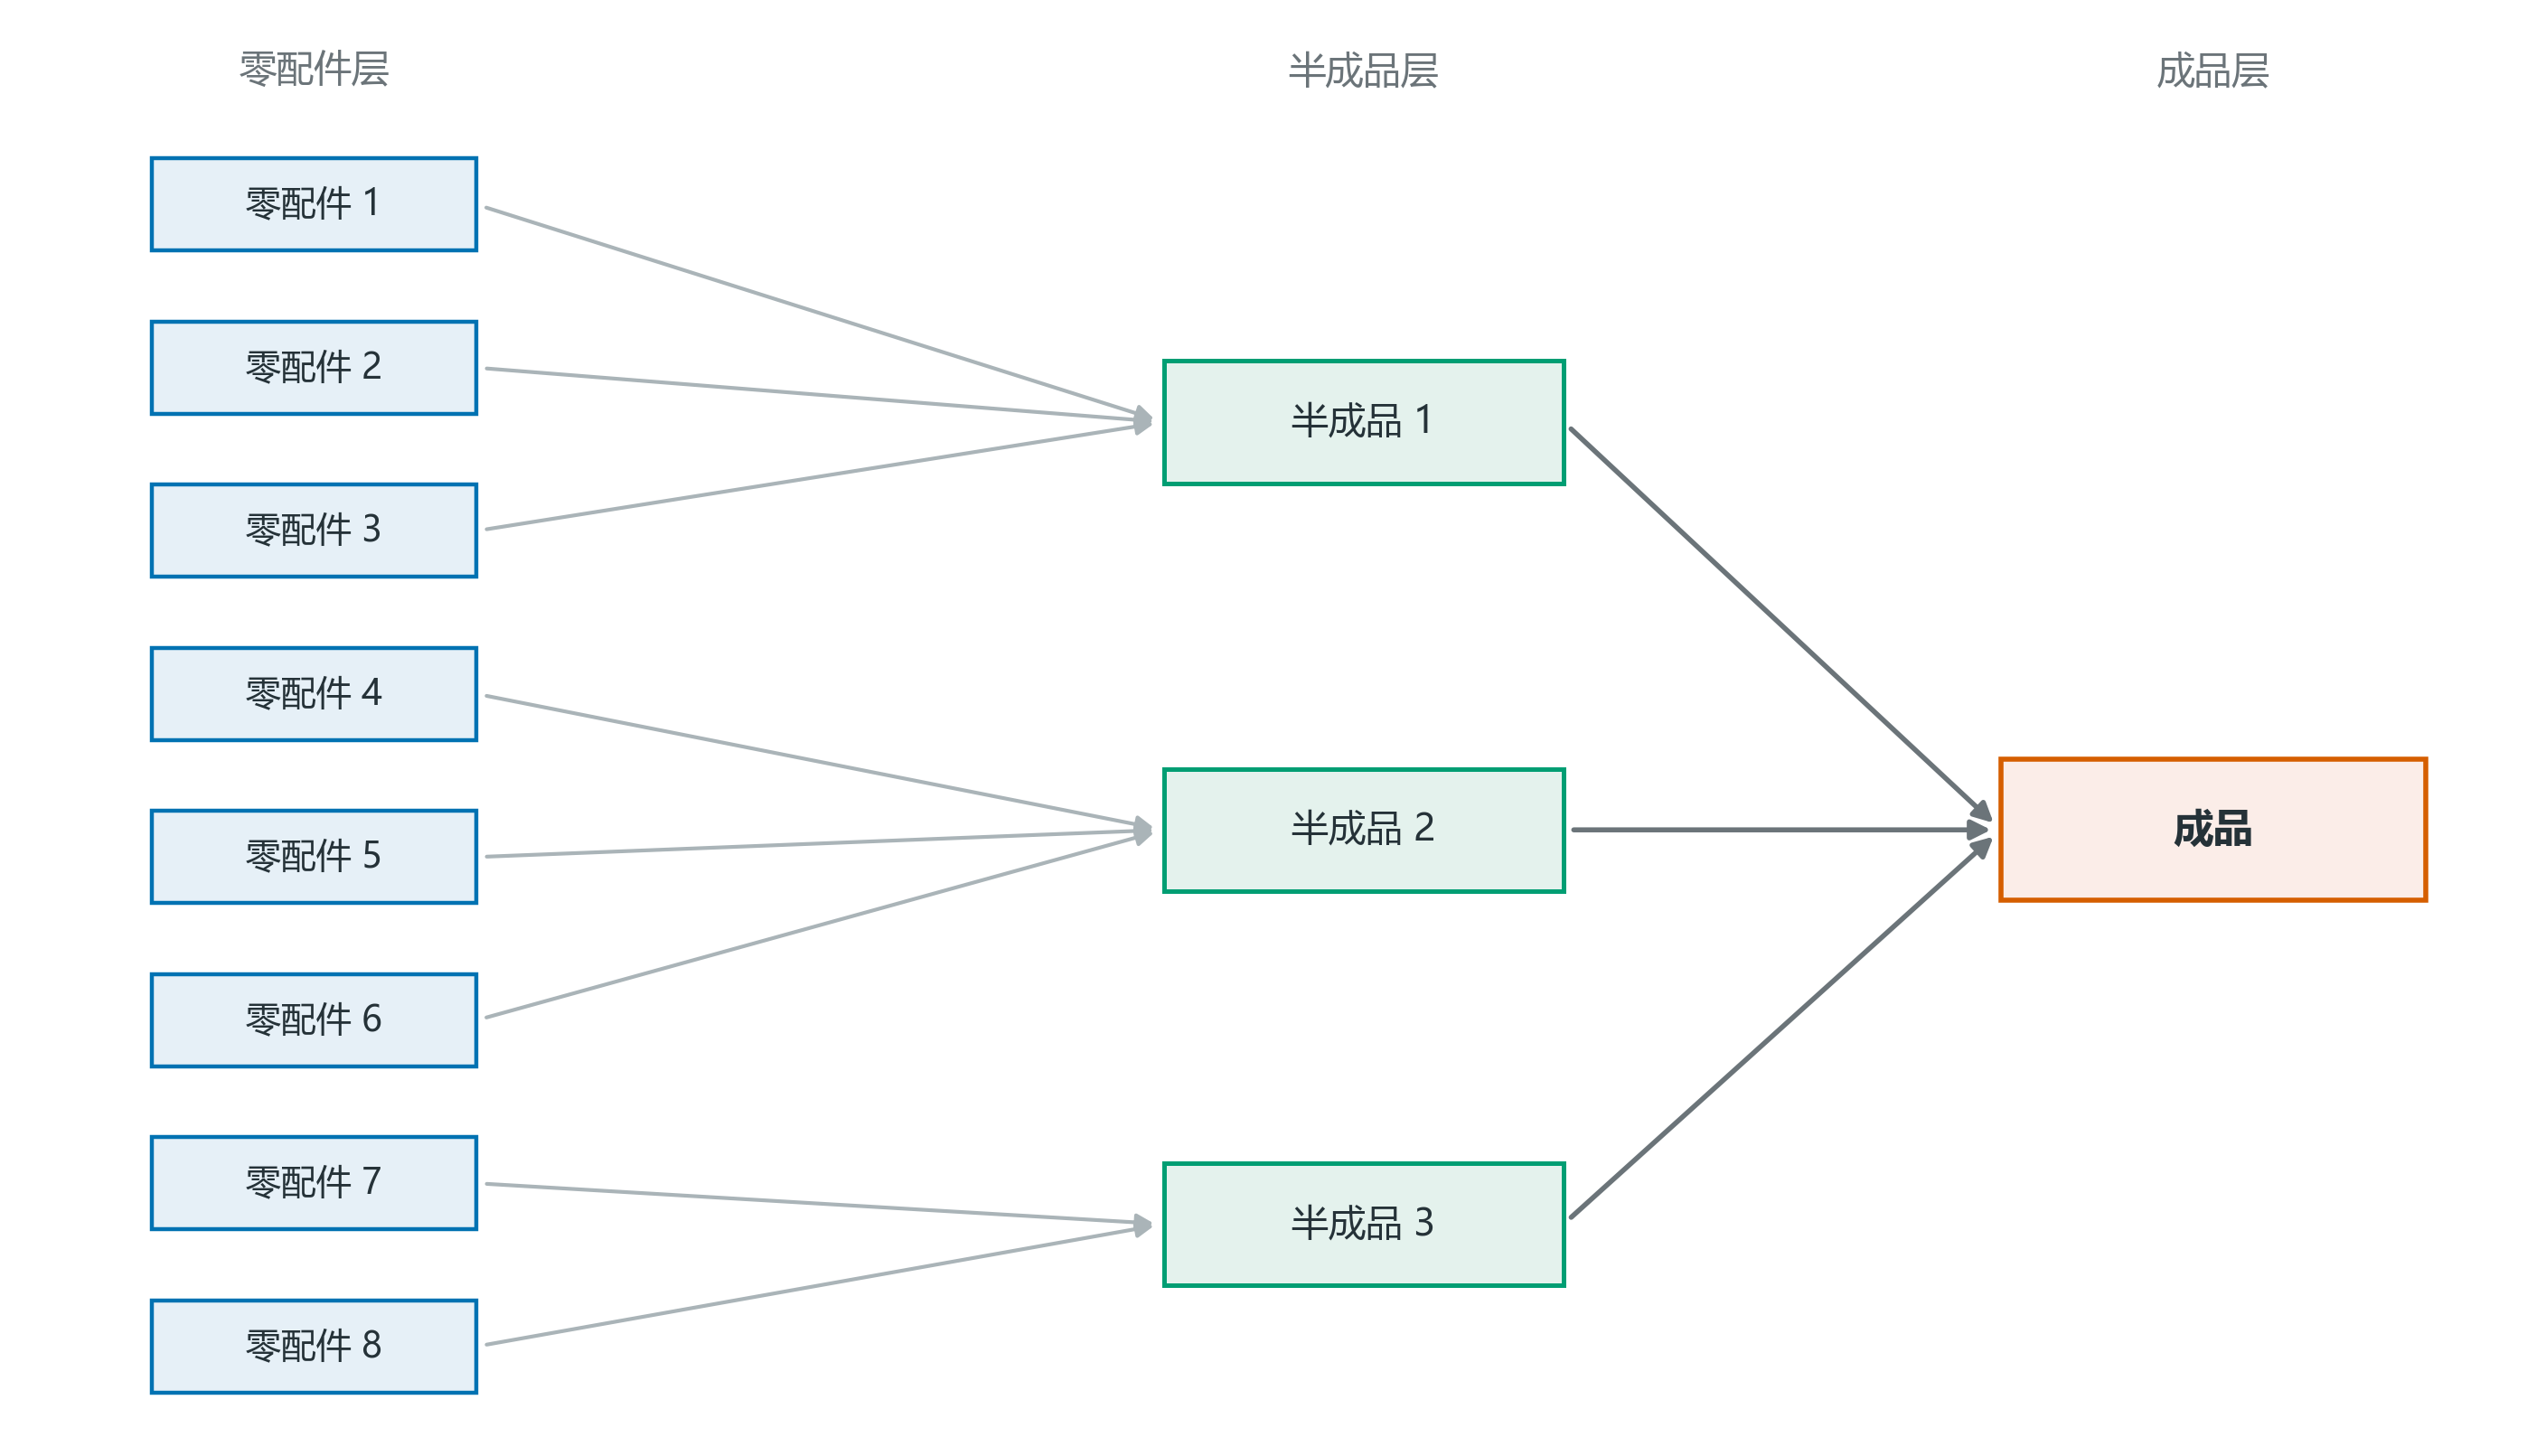
\includegraphics[width=0.95\textwidth]{fig4_flow_3d.png}
    \caption{8 零配件 $\to$ 3 半成品 $\to$ 1 成品的分层装配网络
    结构。底部 8 个零配件按 $\{1,2,3\} \to H_1$、$\{4,5,6\}
    \to H_2$、$\{7,8\} \to H_3$ 的规则分别装配成三个半成品，
    三个半成品再共同装配为成品。每一层级都可独立设置
    "检测/拆解"二元决策，使总决策空间扩展为 $2^{16} = 65\,536$。}
    \label{fig:q3-network}
\end{figure}

题图 1 给出 2 道工序、8 个零配件的装配网络：
\begin{equation}
    \{1, 2, 3\} \to H_1,\quad
    \{4, 5, 6\} \to H_2,\quad
    \{7, 8\} \to H_3,
\end{equation}
三个半成品再共同装配为成品 $F$。

\begin{figure}[htbp]
    \centering
    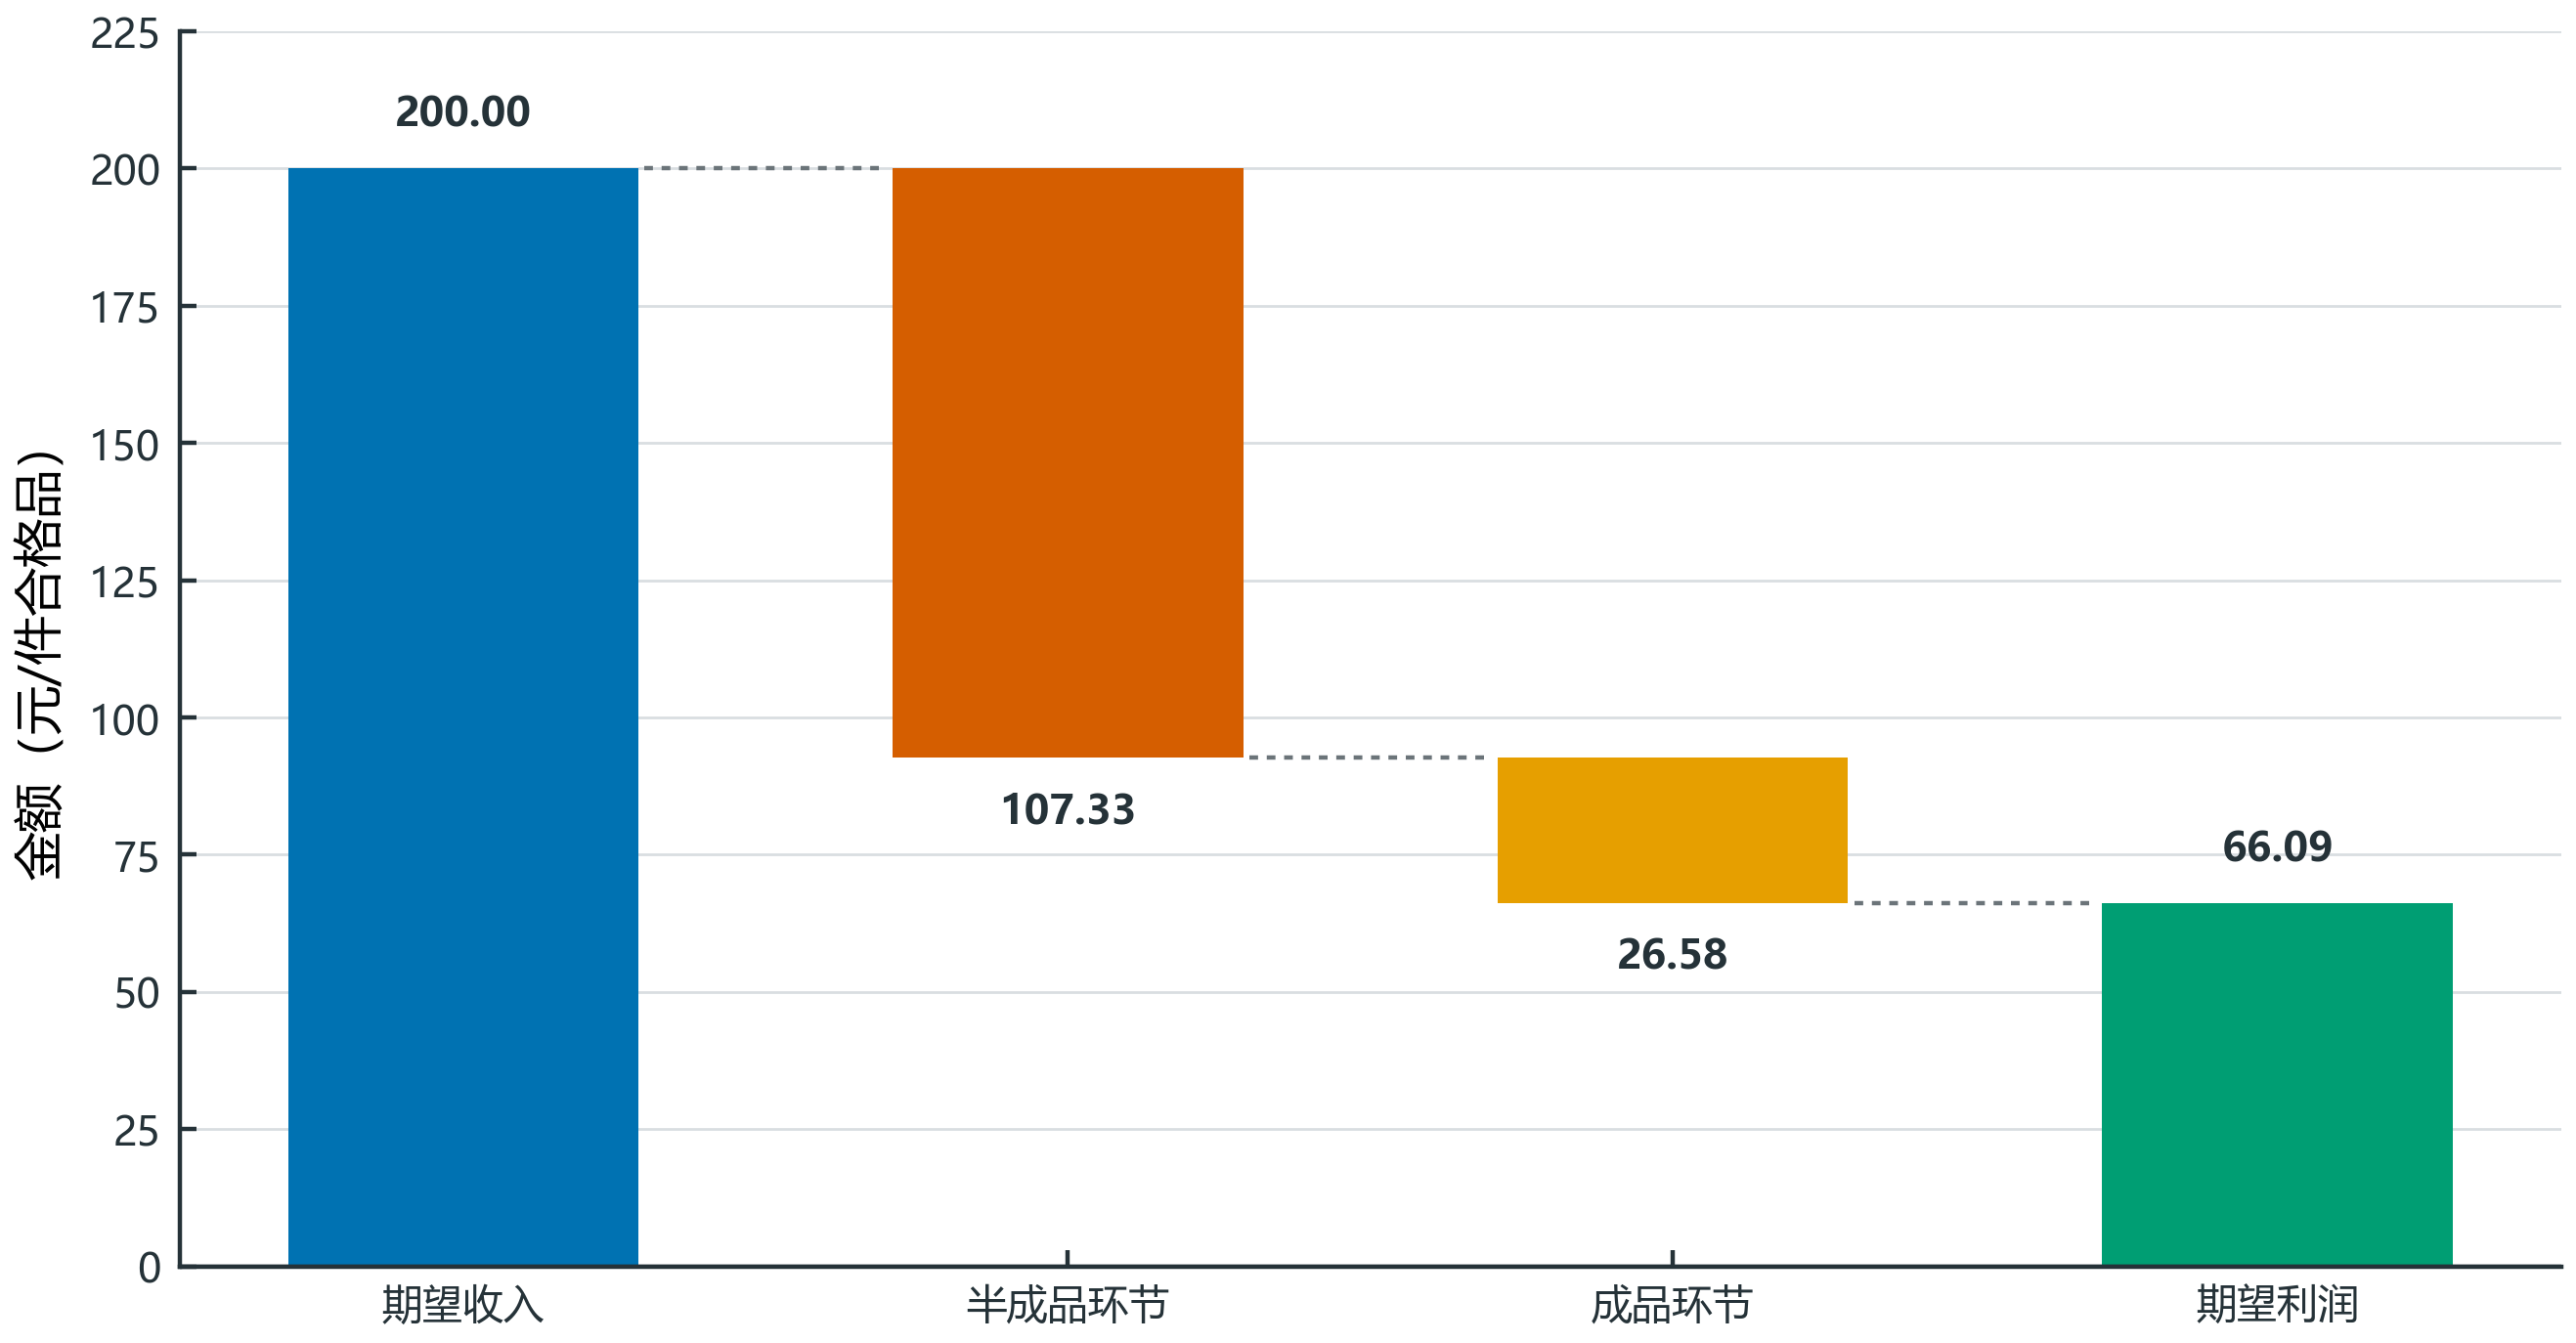
\includegraphics[width=0.78\textwidth]{fig3_cost_structure.png}
    \caption{最优策略 \texttt{11111111|000|000|11} 下的
    期望利润瀑布图。期望收入 200 元依次扣除半成品环节
    107.33 元（含零配件采购与装配）与成品环节 26.58 元
    （含检测、拆解与回收件再处理），得到期望利润
    66.09 元/件合格品。瀑布结构清晰展示两层成本各自
    占比，便于与基准策略的利润差异作来源分析。}
    \label{fig:q3-cost-waterfall}
\end{figure}

本章定义 16 个二元决策变量：
\begin{itemize}
    \item $x_j \in \{0, 1\}$，$j = 1, \ldots, 8$：零配件 $j$ 是否
    检测；
    \item $y_i \in \{0, 1\}$，$i = 1, 2, 3$：半成品 $i$ 是否
    检测；
    \item $z_i \in \{0, 1\}$，$i = 1, 2, 3$：不合格半成品 $i$
    是否拆解；
    \item $y_f \in \{0, 1\}$：成品是否检测；
    \item $z_f \in \{0, 1\}$：不合格成品是否拆解。
\end{itemize}

策略编码统一写作
\begin{equation}
    x_1 \cdots x_8 \mid y_1 y_2 y_3 \mid z_1 z_2 z_3 \mid y_f z_f.
\end{equation}

\textbf{2. 级联质量传播}

零配件 $j$ 进入装配时的实际次品率
\begin{equation}
    e_j = p_j (1 - x_j).
\end{equation}
对半成品 $i$，设其上游零配件集合为 $J_i$，实际不合格率
\begin{equation}
    q_i = 1 - (1 - p_h) \prod_{j \in J_i} (1 - e_j).
\end{equation}
只有未检测半成品的质量风险继续传递，因此成品实际不合格率
\begin{equation}
    q_f = 1 - (1 - p_f) \prod_{i=1}^{3} \bigl[ 1 - q_i (1 - y_i) \bigr].
    \label{eq:q3-qf}
\end{equation}

\textbf{3. 自底向上的期望成本递推}

\textbf{零配件层}：首轮成本与回收件成本
\begin{equation}
    C_j = (1 - x_j) c_j + x_j \frac{c_j + d_j}{1 - p_j}, \quad
    D_j = x_j \frac{d_j + c_j p_j}{1 - p_j}.
\end{equation}

\textbf{半成品层}：若 $y_i = 0$，
\begin{equation}
    E_i = \sum_{j \in J_i} C_j + a_h, \qquad \text{输出次品率 } q_i.
\end{equation}
若 $y_i = 1$，检测会触发循环：
\begin{equation}
    E_i = \frac{
        \sum_{j \in J_i} C_j + a_h + d_h
        + q_i z_i \bigl( \sum D_j - \sum C_j + f_h \bigr)
    }{1 - q_i}.
\end{equation}
回收件再处理成本
\begin{equation}
    R_i = \frac{
        d_h + q_i \bigl[ a_h + z_i \sum D_j + (1 - z_i) \sum C_j + z_i f_h \bigr]
    }{1 - q_i}.
\end{equation}

\textbf{成品层}：令 $B_f = a_f + y_f d_f$。若拆解成品
($z_f = 1$)：
\begin{equation}
    C_f = \sum_{i=1}^{3} E_i + \frac{B_f + q_f (f_f + \sum R_i)}{1 - q_f}.
\end{equation}
若不拆解：
\begin{equation}
    C_f = \frac{\sum E_i + B_f}{1 - q_f}.
\end{equation}
期望收入与目标函数
\begin{equation}
    R_f = \begin{cases}
        s, & y_f = 1, \\[2mm]
        s - \dfrac{q_f r}{1 - q_f}, & y_f = 0.
    \end{cases}
    \quad \pi = R_f - C_f.
\end{equation}

\subsubsection{求解方法}

对全部 $2^{16} = 65\,536$ 种策略枚举并比较利润。Python 实现
采用 NumPy 向量化避免显式循环，约 2 秒完成单情形枚举。

\subsubsection{结果分析}

\textbf{1. 最优有效策略}

\begin{equation}
    \boxed{
    11111111 \mid 000 \mid {-}{-}{-} \mid 11
    }
    \label{eq:q3-opt}
\end{equation}
其中 \texttt{-}{-}{-} 表示三个半成品的拆解决策在 $y = 000$ 时
不会被触发（因为半成品本身未检测，不合格半成品不会在半成品
节点被识别，拆解决策没有触发条件），其取值不影响利润。规范
代表编码记为 $11111111\,|\,000\,|\,000\,|\,11$。

\begin{table}[htbp]
\centering
\caption{问题 3 最优策略的层级决策与经济解释}
\label{tab:q3-decisions}
\small
\begin{tabular}{@{}p{2.0cm}p{4.0cm}p{8.0cm}@{}}
\toprule[1.5pt]
\textbf{层级} & \textbf{最优有效决策} & \textbf{经济解释} \\
\midrule[1pt]
八个零配件 & 全部检测 ($x_j = 1$) &
检测费 1--2 元/件，前端剔除 10\% 次品可避免后续级联损失 \\
三个半成品 & 全部不检测 ($y_i = 0$) &
每个节点检测费 4 元、拆解费 6 元，分散检测成本过高 \\
成品 & 检测并拆解 ($y_f = z_f = 1$) &
高售价（200 元/件）和调换损失（40 元/件）要求保证出厂质量；
拆解可回收高价值半成品 \\
\bottomrule[1.5pt]
\end{tabular}
\end{table}

核心指标：
\begin{equation}
    R = 200.0000,\quad C = 133.9131,\quad
    \pi = 66.0869 \text{ 元/件合格品},\quad
    q_f = 0.3439.
\end{equation}
期望生产轮数 $1/(1 - q_f) = 1.5242$，即平均每交付一件合格品
需要经过 1.52 轮生产。

\textbf{2. 等价最优编码}

Top-20 结果中有 8 个利润完全相同的最优编码，它们仅在
$z_1 z_2 z_3$ 上不同。由于半成品均不检测，拆解决策没有触发
条件，因此这是有效策略相同导致的编码等价类，不是优化算法
出现多个经济含义不同的最优解。论文中报告规范编码
$11111111\,|\,000\,|\,000\,|\,11$ 即可。

\textbf{3. 基准策略比较}

表 \ref{tab:q3-baseline} 给出最优策略与 4 个基准策略的对比。

\begin{table}[htbp]
\centering
\caption{问题 3 最优策略与 4 个基准策略的对比}
\label{tab:q3-baseline}
\small
\begin{tabular}{lrrl}
\toprule[1.5pt]
\textbf{策略} & \textbf{利润（元/件）} & \textbf{$q_f$} & \textbf{简要说明} \\
\midrule[1pt]
最优有效策略 & \textbf{66.09} & 0.3439 & 配件全检、成品集中检测拆解 \\
全部检测 + 全部拆解 & 53.61 & 0.1000 & 半成品层重复检测和拆解成本过高 \\
全部检测 + 不拆解   & 37.12 & 0.1000 & 失败后整体重做成本高 \\
全部不检测 + 成品拆解 & $-43.36$ & 0.7176 & 上游质量失控导致频繁循环 \\
全部不检测 & $-241.54$ & 0.7176 & 高退换损失和重做成本共同累积 \\
\bottomrule[1.5pt]
\end{tabular}
\end{table}

\begin{figure}[htbp]
    \centering
    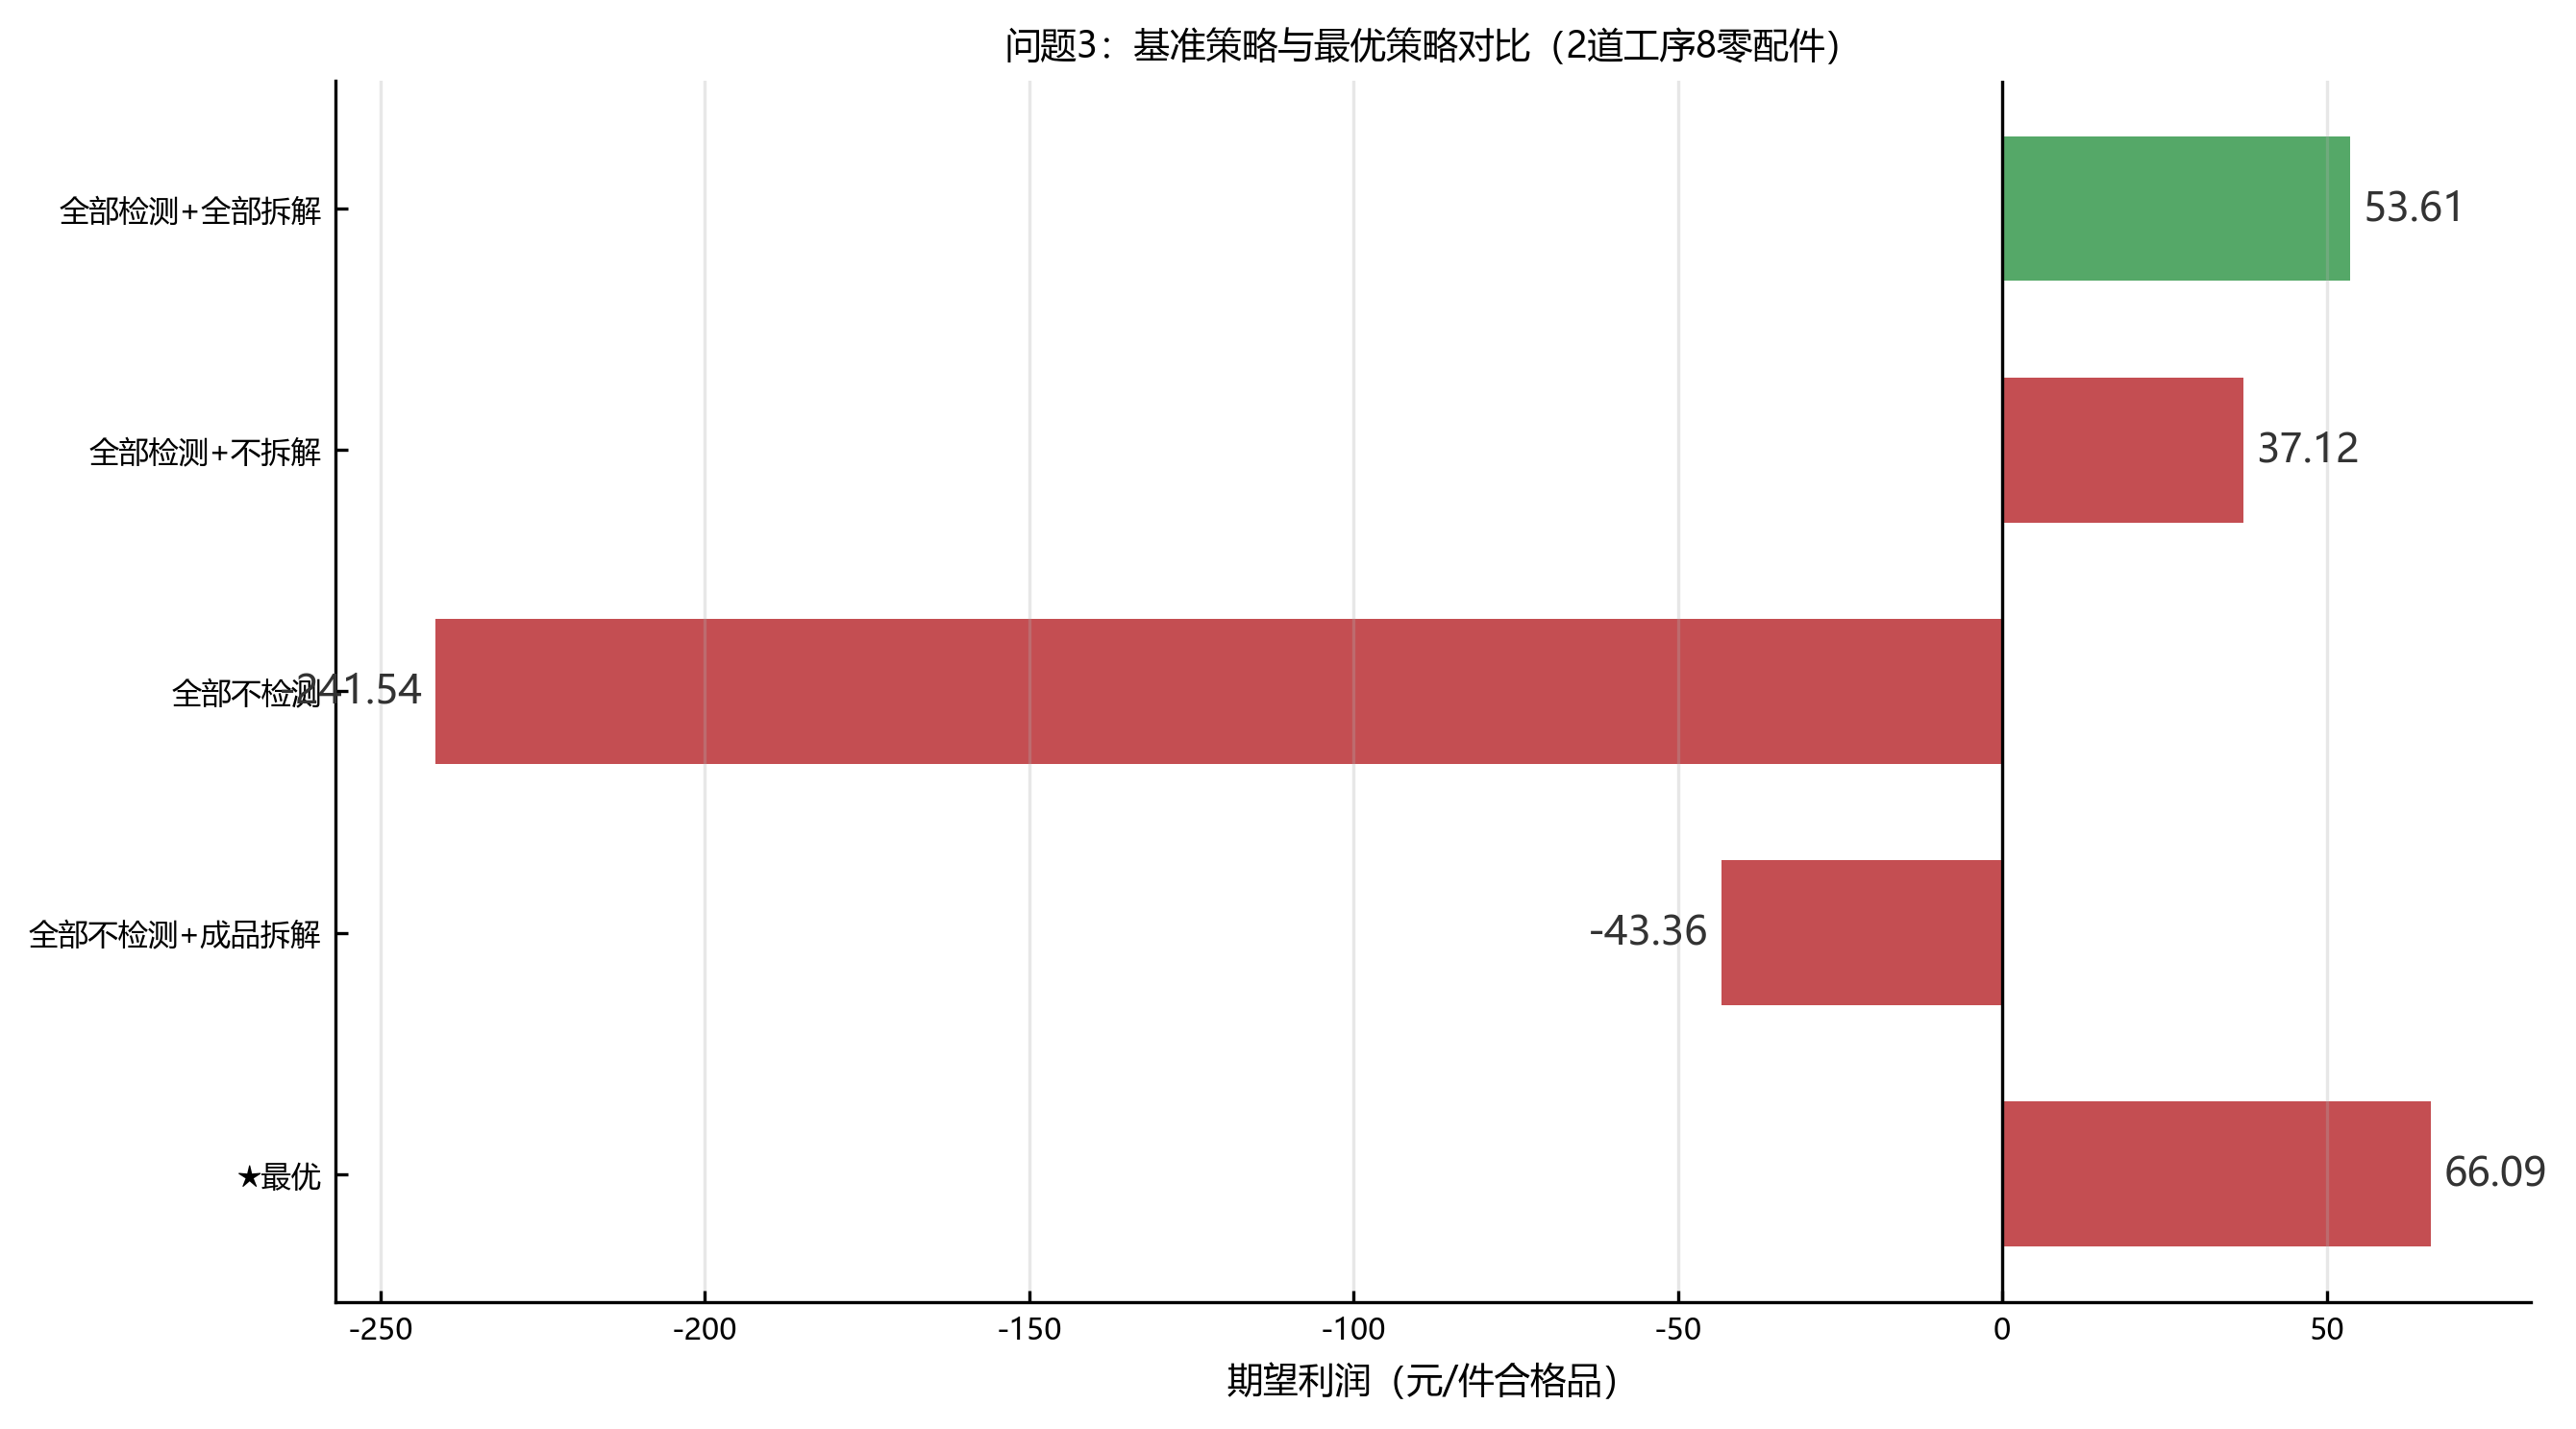
\includegraphics[width=0.95\textwidth]{fig1_baseline_compare.png}
    \caption{最优策略 \texttt{11111111|000|000|11} 与 4 个基准策略的
    利润横向对比。最优策略（绿色）利润 66.09 元/件，领先其它策略
    12.5 元/件以上；\emph{全部检测+全部拆解} 与 \emph{全部检测+不拆解}
    仍为正利润（53.61、37.12 元/件）但被半成品层冗余检测与失败后整体
    重做的成本拖累；\emph{全部不检测+成品拆解} 与 \emph{全部不检测}
    均为显著负利润（$-43.36$、$-241.54$ 元/件），反映上游质量失控
    后的灾难性放大效应。}
    \label{fig:q3-baseline}
\end{figure}

\textbf{4. 质量风险级联放大的直接证据}

在最优策略下所有零配件均检测，三个半成品各自只保留 10\%
的工艺次品率；半成品均不检测，于是
\begin{equation}
    1 - q_f = 0.9^4 = 0.6561, \qquad q_f = 0.3439.
\end{equation}
这一计算是"质量风险级联放大"的直接证据：单节点 10\% 的风险
经过 4 次组合后，使成品不合格率达到 34.39\%。

\subsubsection{模型检验}

\textbf{1. 蒙特卡洛验证}

20 万次蒙特卡洛逐件模拟中，最优策略的模拟利润为 66.1292 元/件，
相对解析值 66.0869 元/件的相对误差仅 0.064\%；五个代表策略
的最大相对误差 0.648\%。该结果同时验证了级联概率和嵌套循环
成本公式的数值正确性。

\textbf{2. 决策骨架的稳定区间}

通过在售价 $S \in [80, 320]$、半成品拆解费 $F_H \in [1, 25]$、
成品拆解费 $F_F$ 与半成品检测费 $D_H$ 上的多参数扫描，可以
观察到最优策略骨架的稳定与迁移：
\begin{itemize}
    \item 售价 $S = 80 \sim 320$ 时，最优策略骨架保持不变；
    \item 半成品拆解费 $F_H = 1 \sim 25$ 时，因半成品本身
    不检测，相关拆解决策不触发，骨架保持不变；
    \item 成品拆解费 $F_F$ 增大时，控制重心由"成品拆解兜底"
    逐步向半成品检测迁移；
    \item 半成品检测费 $D_H$ 足够低时，分散在中间层的检测
    变得经济，零配件检测数量也随之调整。
\end{itemize}
这说明"下游集中兜底"不是绝对规律，而是在当前检测费、
拆解费结构下的最优组织方式。当经济参数发生量级变化时，
决策骨架可能向"分散拦截"方向迁移。

\begin{figure}[htbp]
    \centering
    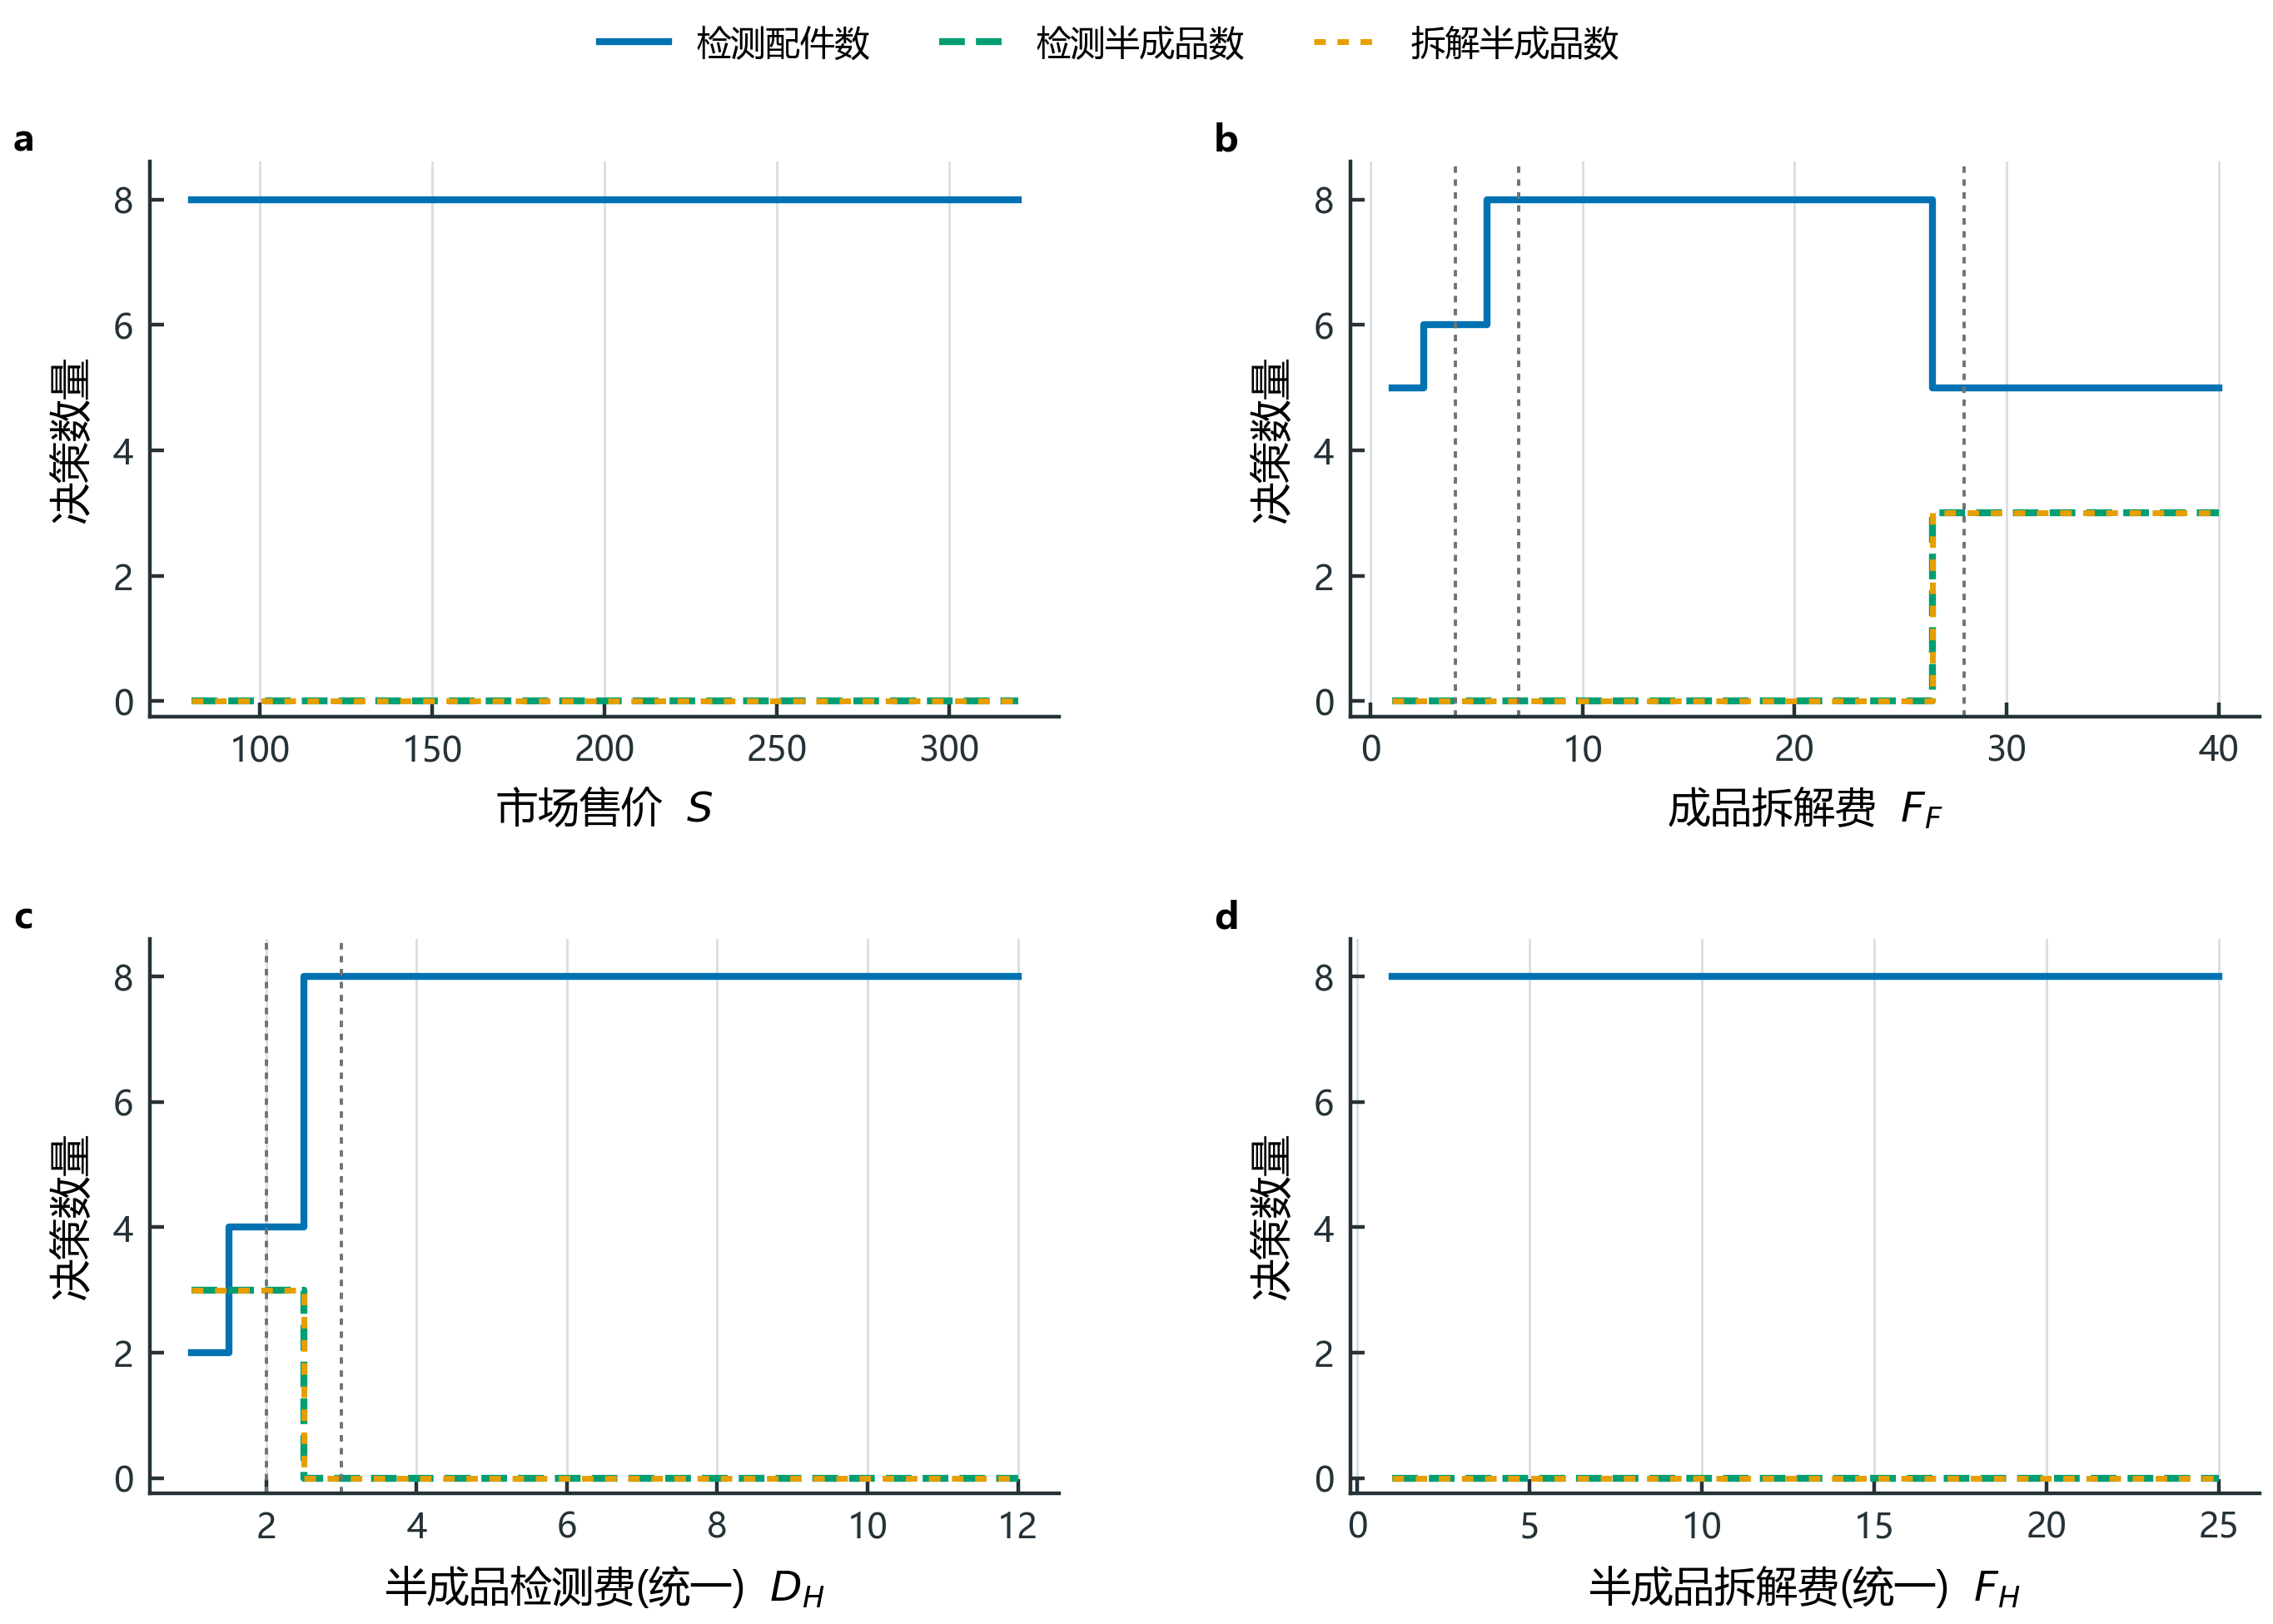
\includegraphics[width=0.95\textwidth]{fig5_sensitivity.png}
    \caption{多参数敏感性下最优策略中"检测"决策数量的
    阶跃变化。横轴分别扫描售价 $S$、半成品检测费 $D_H$、
    半成品拆解费 $F_H$、成品拆解费 $F_F$。在 $S \in [80, 320]$
    与 $F_H \in [1, 25]$ 区间内骨架稳定（8 个配件检测 +
    3 个半成品不检测 + 成品检测拆解）；$F_F$ 增大触发
    骨架向半成品检测迁移，$D_H$ 极低时骨架向"分散拦截"
    方向迁移。虚线标注当前默认参数位置。}
    \label{fig:q3-sensitivity}
\end{figure}

\textbf{3. 浅层决策树的辅助验证}

在 150 组参数样本中，各零配件进入最优检测集合的频率约为
64\%--96\%。检测费为 1 元的零配件被检测概率约 91\%--96\%，
检测费为 2 元的高价零配件约 64\%--67\%。浅层决策树在留出集
上的准确率约 88\%，主要阈值涉及次品率 $p_j$、检测费 $d_j$ 和
成品拆解费 $F_F$。浅层决策树只是对 65\,536 策略枚举结果
的可解释压缩，论文结论仍以全枚举为准。

\subsubsection{单比特翻转检验}

全枚举只能保证全局最优性，不直接展示各决策变量对利润的边际
贡献。对最优编码 $11111111\,|\,000\,|\,000\,|\,11$ 逐一翻转
16 个决策变量，记录翻转后利润：

\begin{itemize}
    \item 13 个翻转后利润下降（\emph{关键} 决策）；
    \item 3 个翻转后利润不变（$z_1, z_2, z_3$，因 $y = 000$ 不触发，
    实证了 §5.3.3 等价最优编码类）；
    \item 0 个翻转后利润上升（无遗漏解）。
\end{itemize}

\begin{figure}[htbp]
    \centering
    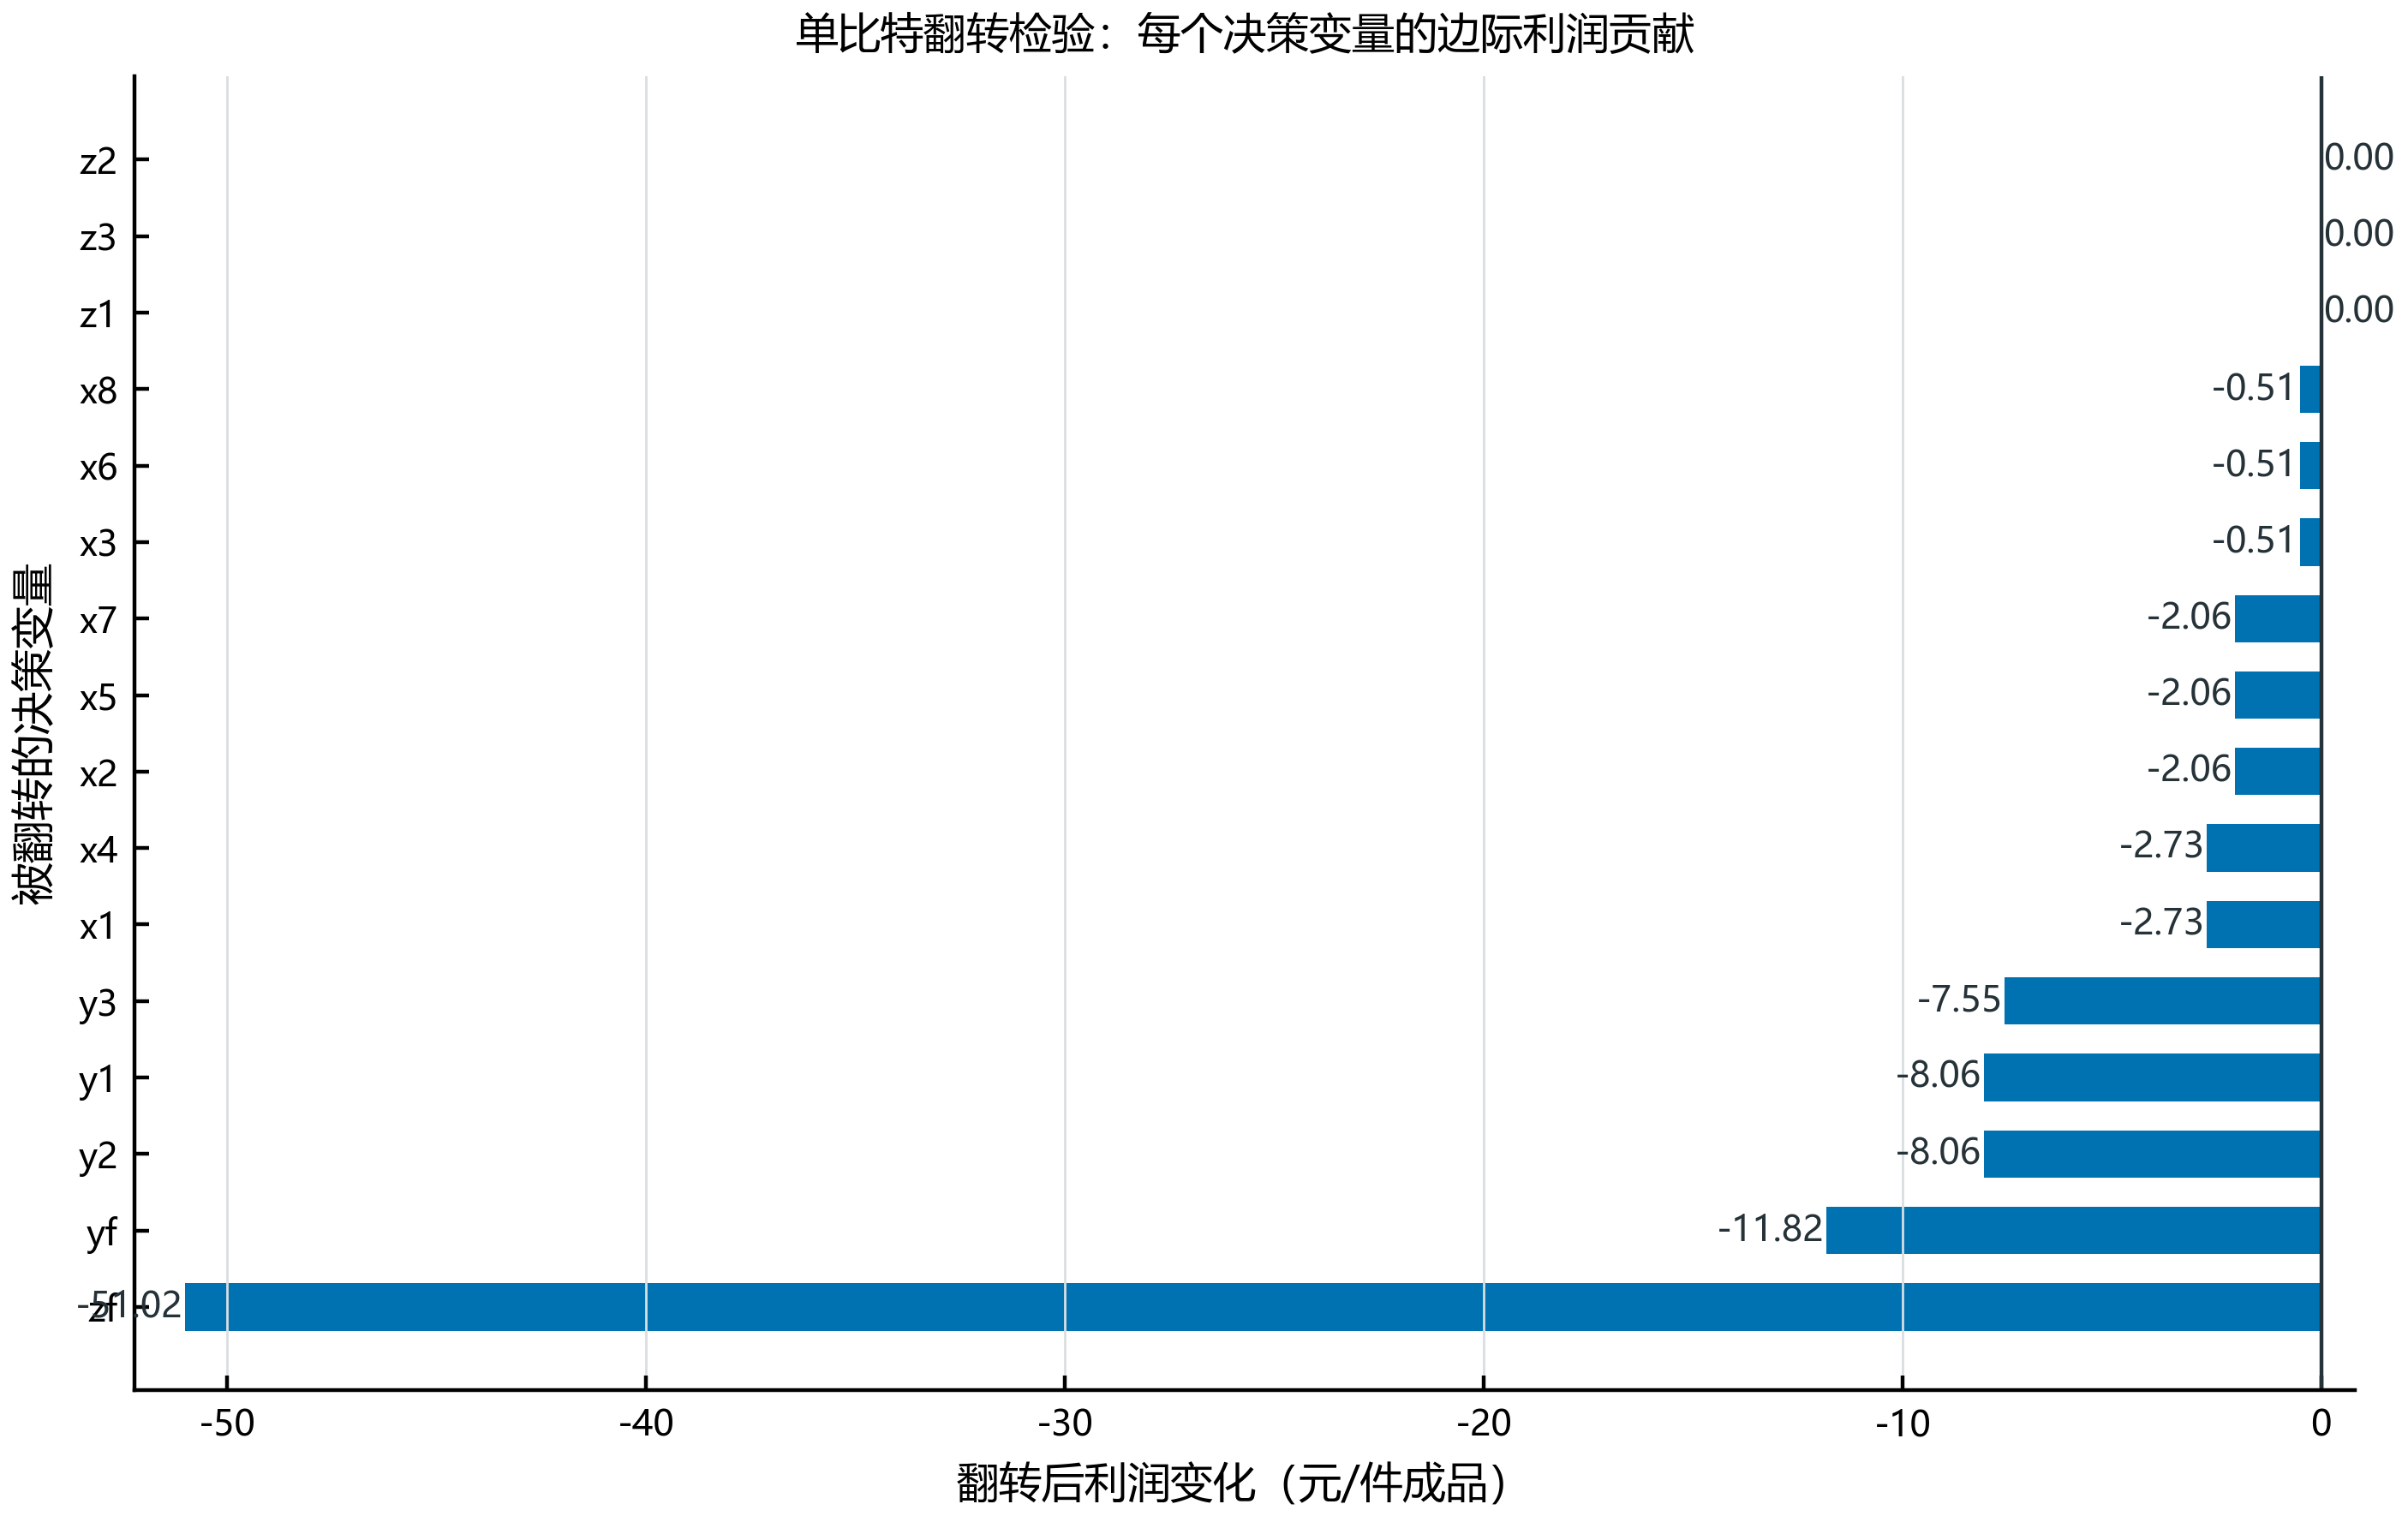
\includegraphics[width=0.92\textwidth]{fig6_flip_check.png}
    \caption{对最优编码逐一翻转 16 个决策变量的边际利润损失。
    纵轴按损失量降序：成品拆解 $z_f$（51.02 元/件，翻转后
    利润由 66.09 崩至 15.07） $>$ 成品检测 $y_f$（11.82）$
    >$ 半成品检测 $y_1, y_2$（8.06）、$y_3$（7.55）$>$
    零配件检测 $x_1$--$x_8$（0.51--2.73，便宜件高于贵件）。
    $z_1, z_2, z_3$ 损失为 0，验证等价编码类无实质差异。}
    \label{fig:q3-flip-check}
\end{figure}

边际价值排序与"下游集中兜底"的经济直觉一致：成品拆解
承担了几乎全部下游兜底责任（贡献过半），半成品层只在不
触发时冗余，零配件层各变量贡献相近且与单价弱相关。
13 降 + 3 不变 + 0 上升同时验证了局部最优的稳定性，与全
枚举共同保证全局最优。

%% ---------- 问题四 ----------
\subsection{问题四的建模与求解}
\label{sec:q4}

\subsubsection{模型构建}

问题 4 不是简单地把次品率替换成一个抽样估计值后重算问题 2，
而是要回答：抽多少、观察到什么、据此如何改变生产决策，以及
信息是否值得其成本。因此将抽样内生化到决策链：

\begin{equation}
\begin{aligned}
    &\text{先验质量认知} \;\to\; \text{选择抽样量} \;\to\; \text{获得观测} \\
    &\;\to\; \text{更新次品率分布} \;\to\; \text{重选生产策略} \;\to\; \text{评价信息净价值}.
\end{aligned}
\end{equation}

\textbf{1. Beta--Binomial 共轭模型}

对问题 2 中的三个次品率参数 $p_1, p_2, p_0$ 分别设置独立
Beta 先验：
\begin{equation}
    p_j \sim \mathrm{Beta}(a_{0j}, b_{0j}), \qquad
    a_{0j} = \hat p_j n_{\mathrm{prior}}, \quad
    b_{0j} = (1 - \hat p_j) n_{\mathrm{prior}}.
\end{equation}
其中先验均值 $\hat p_j$ 等于题表值，默认等价样本量
$n_{\mathrm{prior}} = 30$。

对每个参数抽检 $n$ 件，观测次品数 $k_j \mid p_j \sim \mathrm{Bin}(n, p_j)$。
由共轭性，后验分布仍为 Beta：
\begin{equation}
    p_j \mid k_j, n \sim \mathrm{Beta}(a_{0j} + k_j,\; b_{0j} + n - k_j).
\end{equation}

\textbf{2. 观测驱动的生产决策}

给定观测向量 $\mathbf{k} = (k_1, k_2, k_0)$，重新评价问题 2 的 16 种策略：
\begin{equation}
    x^\star(\mathbf{k}, n) = \arg\max_{x \in \{0,1\}^4}
    \E_{p \mid \mathbf{k}, n} \bigl[ \pi(p, x) \bigr].
    \label{eq:q4-obs}
\end{equation}
因此生产策略不再是固定值，而是观测结果的函数。

\textbf{3. 事前价值与最优抽样量}

对抽样前所有可能的真实次品率和观测结果取期望：
\begin{equation}
    V(n) = \E_{p, \mathbf{k}}\Bigl[\;
        \max_{x} \E_{p \mid \mathbf{k}, n} \bigl[ \pi(p, x) \bigr]
    \Bigr] - \frac{3 n d}{B}.
    \label{eq:q4-Vn}
\end{equation}
其中 $3n$：三个次品率参数各抽 $n$ 件；$d$：单件检测成本；
$B$：生产批量；$3nd / B$：每批抽样成本摊到每件成品后的成本。

最优抽样量与信息净价值
\begin{equation}
    n^\star = \arg\max_{n \in \mathcal{N}} V(n), \qquad
    \mathrm{EVSI} = V(n^\star) - V(0),
\end{equation}
其中 $\mathcal{N} = \{0, 10, 20, \ldots, 100\}$。

\subsubsection{求解方法}

为减小 $V(n)$ 曲线的比较方差，本文采用共同随机数（CRN）
方法：
\begin{enumerate}
    \item 外层从先验中生成质量"世界"；
    \item 对各候选 $n$ 在同一外层世界下生成相应观测；
    \item 内层从后验抽样，计算 16 种策略的后验期望利润；
    \item 使用同一组随机数评价所有候选 $n$；
    \item 扣除抽样成本后选取最大值。
\end{enumerate}
默认使用 300 个外层世界、500 个后验样本，随机种子 2024。

\subsubsection{结果分析}

\textbf{1. 默认参数结果}

默认设定：$n_{\mathrm{prior}} = 30$、$d = 2$ 元/件、$B = 1000$ 件/批。
表 \ref{tab:q4-default} 给出六情形下的最优抽样量与 EVSI。

\begin{table}[htbp]
\centering
\caption{默认参数下六情形的最优抽样量与 EVSI}
\label{tab:q4-default}
\small
\begin{tabular}{ccccc}
\toprule[1.5pt]
情形 & $n^\star$ & $V(n^\star)$ & $V(0)$ & $\mathrm{EVSI}$（元/件） \\
\midrule[1pt]
1 & 0  & 21.413 & 21.413 & 0.000 \\
2 & \textbf{10} & 12.359 & 12.310 & \textbf{0.049} \\
3 & 0  & 19.576 & 19.576 & 0.000 \\
4 & 0  & 14.690 & 14.690 & 0.000 \\
5 & 0  & 18.602 & 18.602 & 0.000 \\
6 & 0  & 21.423 & 21.423 & 0.000 \\
\bottomrule[1.5pt]
\end{tabular}
\end{table}

默认条件下只有情形 2 值得进行少量抽样，其余情形均选择不抽样。
原因不是抽样完全没有统计信息，而是这些信息很少改变最优生产
策略，或改变策略带来的毛收益不足以覆盖抽样成本。这体现了
"利润平台效应"：策略标签可能随估计变化，但若候选策略利润
接近，错误选择的经济损失仍然很小。

情形 2 的 EVSI 为 0.049 元/件，对 1000 件批量约对应 49 元/批
的净期望增益。

\begin{figure}[htbp]
    \centering
    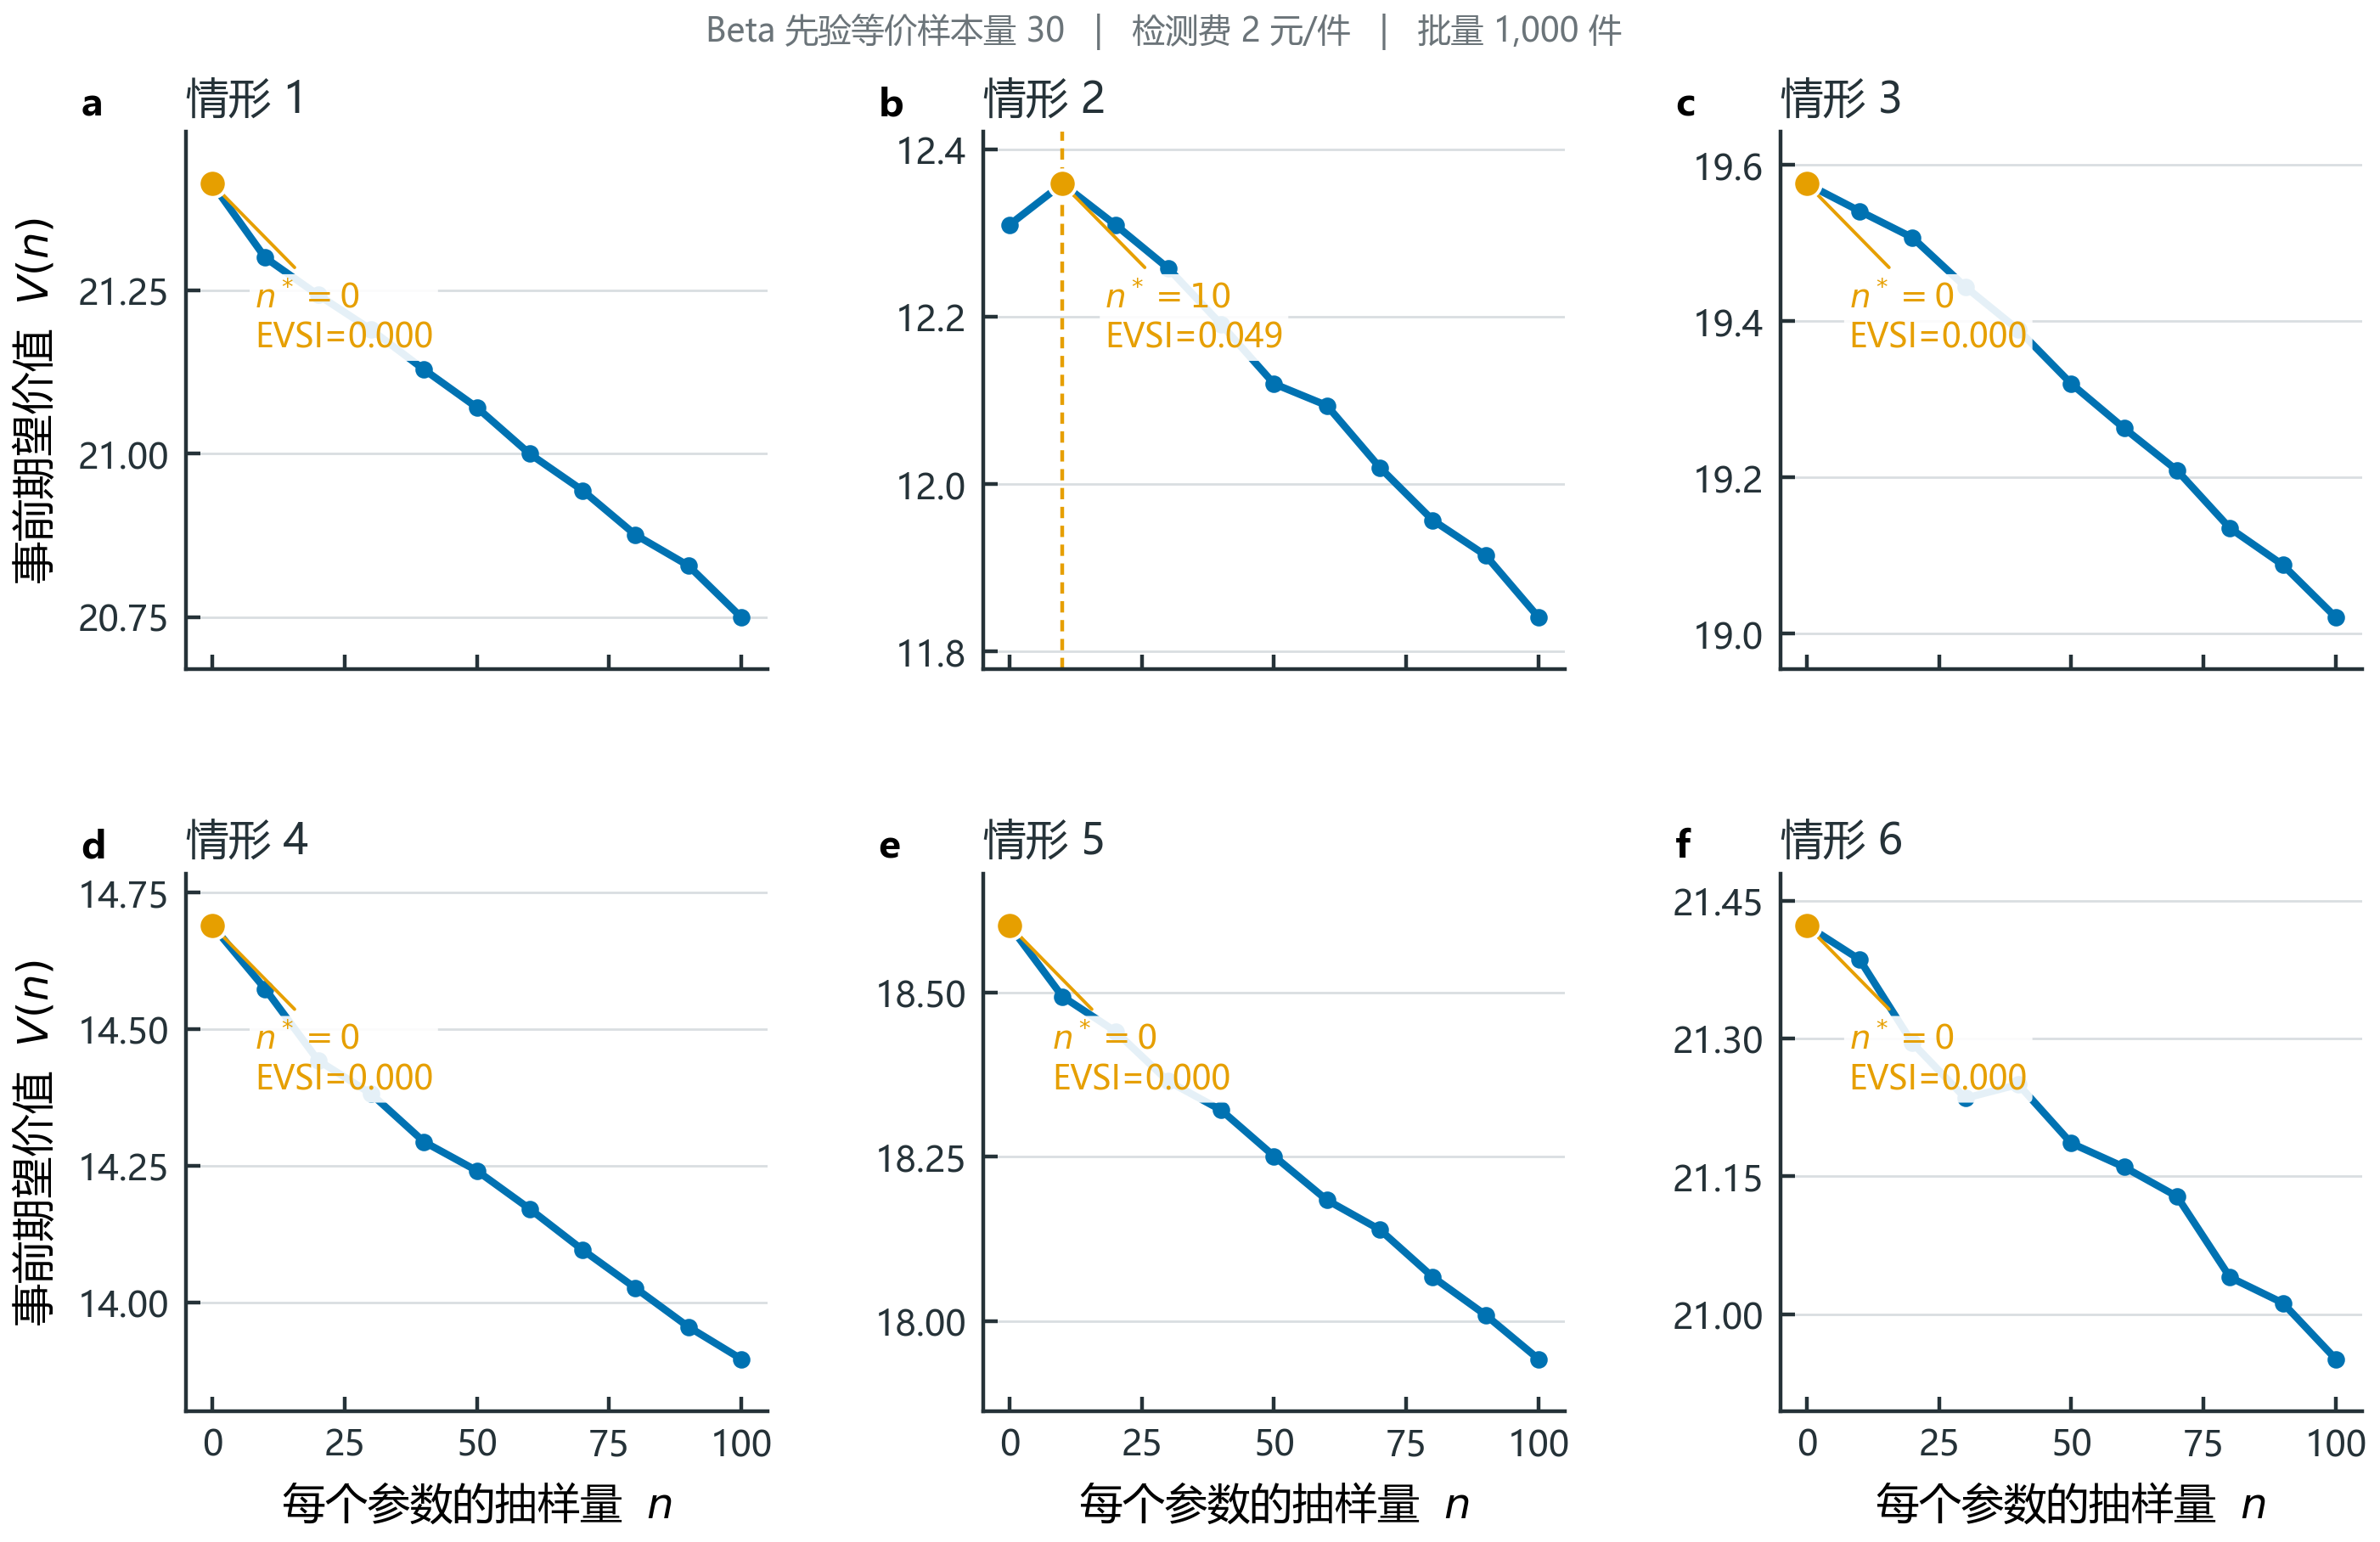
\includegraphics[width=0.95\textwidth]{fig5_evsi.png}
    \caption{6 种情形下事前期望价值 $V(n)$ 随抽样量 $n$ 的变化。
    横轴为每个参数的抽样量 $n$，纵轴为 $V(n)$（元/件），
    橙点标注最优抽样量 $n^\star$。仅情形 2 的 $n^\star = 10$
    使 $V(n)$ 较不抽样时提升 0.049 元/件，其余 5 种情形
    $V(0) \ge V(n)$，最优决策为不抽样。}
    \label{fig:q4-evsi}
\end{figure}

\textbf{2. 批量与检测成本的经济相图}

为揭示抽样的经济可行域，对情形 1、6 扫描
\begin{equation}
    B \in \{100, 1000, 10000\}, \quad
    d \in \{0.5, 2, 5\}.
\end{equation}

\begin{figure}[htbp]
    \centering
    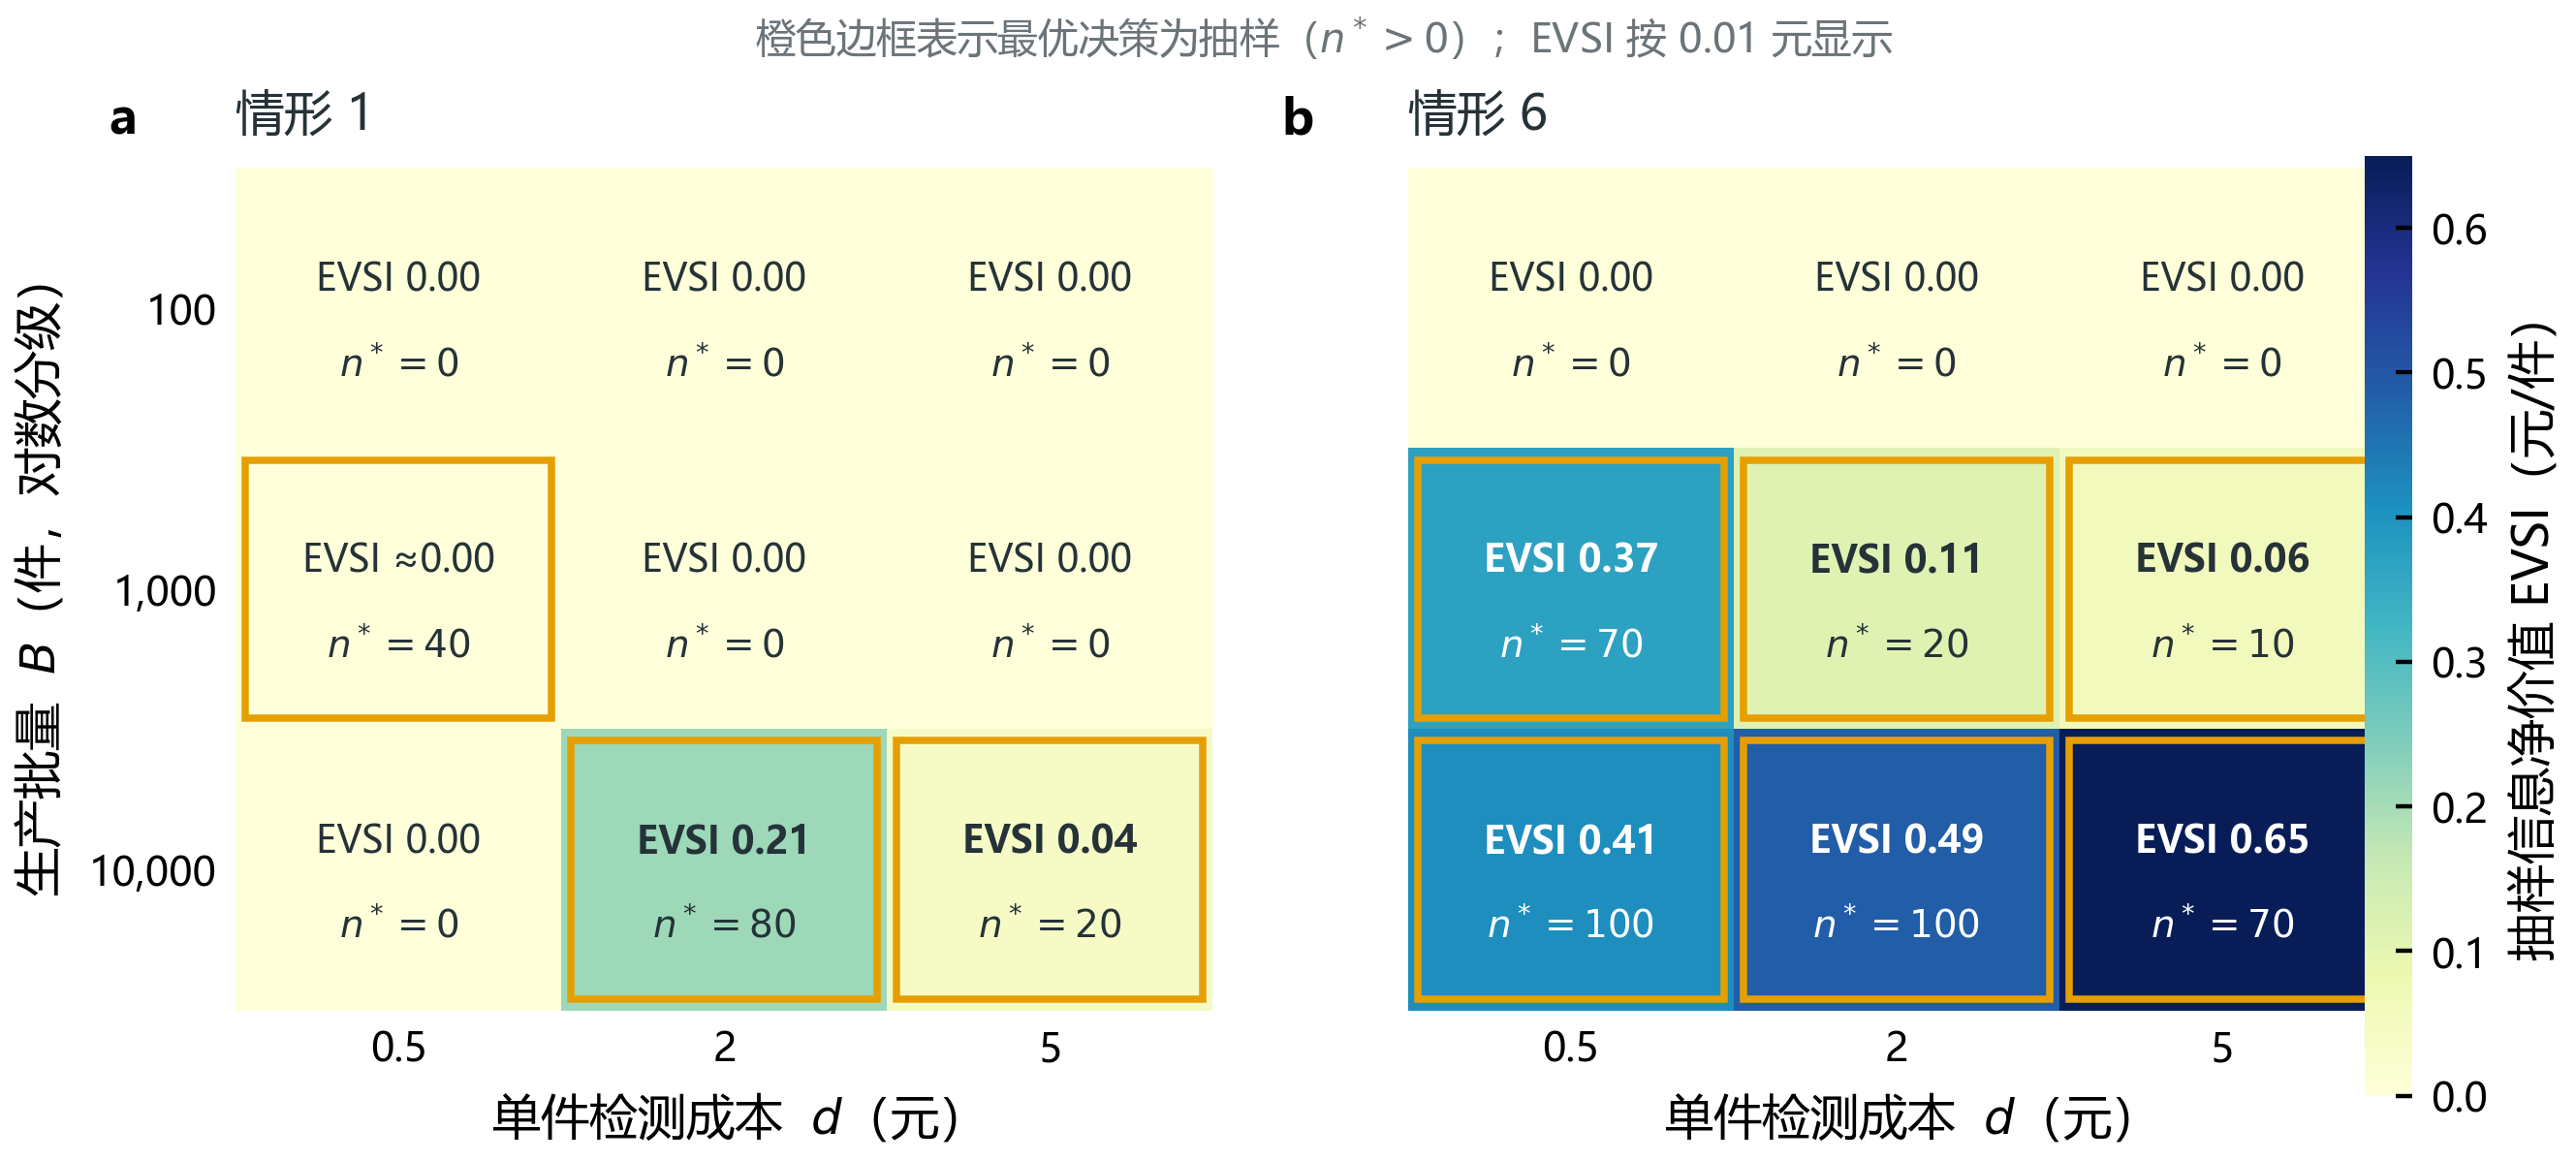
\includegraphics[width=\textwidth]{fig_evsi_phase_map.png}
    \caption{6 种情形在 \emph{检测成本 $d$}--\emph{生产批量 $B$} 平面上的
    EVSI 相图。每个子图 $3 \times 3$ 网格单元的颜色表示 EVSI 大小，
    橙色边框表示该经济参数下最优决策为抽样（$n^\star > 0$）。
    随 $B$ 增大、$d$ 减小，EVSI 上升、最优抽样量增大；
    情形 6 在 $B = 10000$、$d = 5$ 时 EVSI 达 0.65 元/件、
    $n^\star = 70$，是全参数空间中信息价值最高的工况；在
    $d = 0.5$ 时最优抽样量达到扫描上限 $n^\star = 100$。}
    \label{fig:q4-phase}
\end{figure}

情形 6 的结果最具代表性（表 \ref{tab:q4-batchd}）：

\begin{table}[htbp]
\centering
\caption{情形 6 在批量--检测成本平面上的最优抽样量与 EVSI（元/件）}
\label{tab:q4-batchd}
\small
\begin{tabular}{cccc}
\toprule[1.5pt]
$B$（件/批） & $d = 0.5$ & $d = 2$ & $d = 5$ \\
\midrule[1pt]
100   & $(n^\star = 0,\, 0.00)$ & $(0,\, 0)$ & $(0,\, 0)$ \\
1000  & $(70,\, 0.37)$ & $(20,\, 0.11)$ & $(10,\, 0.06)$ \\
10000 & $(100,\, 0.41)$ & $(100,\, 0.49)$ & $(70,\, 0.65)$ \\
\bottomrule[1.5pt]
\end{tabular}
\end{table}

对应每批净收益：$B = 1000$ 约 60 $\sim$ 370 元/批，$B = 10000$
约 4100 $\sim$ 6500 元/批。

\textbf{3. 管理解释}

\begin{enumerate}
    \item \textbf{批量是主导变量}。抽样成本按批发生，批量越大，
    单位产品承担的成本越低。这是情形 6 在 $B = 10000$ 时 EVSI
    显著放大的根本原因。
    \item \textbf{检测成本与最优样本量不必严格单调}。EVSI 由
    离散样本量、策略翻转阈值和蒙特卡洛估计共同决定，不能仅
    凭单调直觉解释每个格点。
    \item \textbf{情形差异来自决策敏感度}。情形 6 在参数不确定
    时更容易跨越策略边界，因此信息更可能改变有经济后果的
    决策；不应简单归因于"次品率越低，先验方差越大"。
    \item \textbf{近零 EVSI 的解释}。情形 1 在 $(B = 1000, d = 0.5)$
    时出现 $n^\star = 40$ 但 EVSI 按两位小数显示为 0.00。
    此时候选方案差值小于显示精度，可能处于蒙特卡洛误差量级，
    应写作"经济上近似无差异"。
\end{enumerate}

\textbf{4. 观测—决策规则}

式 \ref{eq:q4-obs} 给出的决策表自动由后验期望利润产生：
当某一零配件样本中观察到更多次品时，相应后验次品率上升，
前端检测的预期收益增加，最优策略可能由"不检测该配件"切换
为"检测该配件"。该规则无需人工设定，是后验优化的自然产物。

以情形 1 与情形 3 为例，给出两个观测驱动的策略翻转：

\begin{itemize}
    \item \textbf{情形 1}：观测 $(k_1, k_2, k_0) = (0,0,0)$ 时
    最优策略为 $(0,0,0,1)$（不检测任一零配件，仅拆解不合格
    成品）；当 $k_1$ 升至 2 时，最优策略切换为
    $(1,0,0,1)$，即开启配件 1 检测。这是后验次品率上升
    触发前端检测的典型例证。
    \item \textbf{情形 3}：观测 $(k_1, k_2, k_0) = (0,0,0)$
    至 $(2,1,0)$ 时，最优策略保持为 $(0,0,1,1)$；当
    三个参数同时出现 $k = (3,1,1)$ 时，最优策略切换为
    $(1,0,1,1)$，即在原有基础上额外检测配件 1。
    后验联合次品率显著偏离先验均值时，决策表给出更
    强干预的方案。
\end{itemize}

决策表见附录 \ref{app:q4-table}。

\subsubsection{模型检验}

\textbf{1. 与问题 1 样本量的关系}

问题 1 和问题 4 的样本量不同并不矛盾：问题 1 按可靠度阈值
确定验收方案（$n_1 = 29$、$n_2 = 22$），问题 4 按利润最大化
决定信息采集量（默认情形 2 $n^\star = 10$），目标函数不同。
两个问题的关系是：问题 1 给出统计判定的物理基础，问题 4 在
此基础上将信息获取纳入经济决策。问题 4 的"不抽样"决策并不
否认问题 1 抽样方案的有效性，只是说明在当前参数下，抽样
带来的统计信息很少改变最优生产策略。

\textbf{2. 与问题 2、3 的关系}

问题 4 直接调用问题 2 的利润函数 $\pi(p, x)$ 与 16 策略决策
空间。该框架同样适用于问题 3：只需将 $\pi$ 替换为问题 3 的
多级装配期望利润，$x$ 扩展为 16 维决策，EVSI 仍可类似计算
但计算量随状态空间扩大显著增加。

\textbf{3. 局限与改进}

\begin{itemize}
    \item 三个次品率先验相互独立，未考虑共同供应商或工艺
    造成的相关性；
    \item 先验强度 30 具有主观性，应进一步做 $n_{\mathrm{prior}}$
    敏感性；
    \item $n$ 只按 10 的步长扫描，精细最优值需在候选点附近
    二次搜索；
    \item 当前蒙特卡洛结果未同时输出标准误，小 EVSI 的统计
    分辨率有限；
    \item 抽样只考虑一次性静态决策，可扩展为逐批更新、
    贝叶斯控制图或序贯停止。
\end{itemize}

\subsubsection{多种子稳定性检验}

§5.4.3 的 EVSI 估计依赖单一随机种子（2024）。为检验结论的
随机性稳健程度，对情形 1、2、6 重新以 10 个独立随机种子、
每种子 200 个外层世界运行，结果如下：

\begin{figure}[htbp]
    \centering
    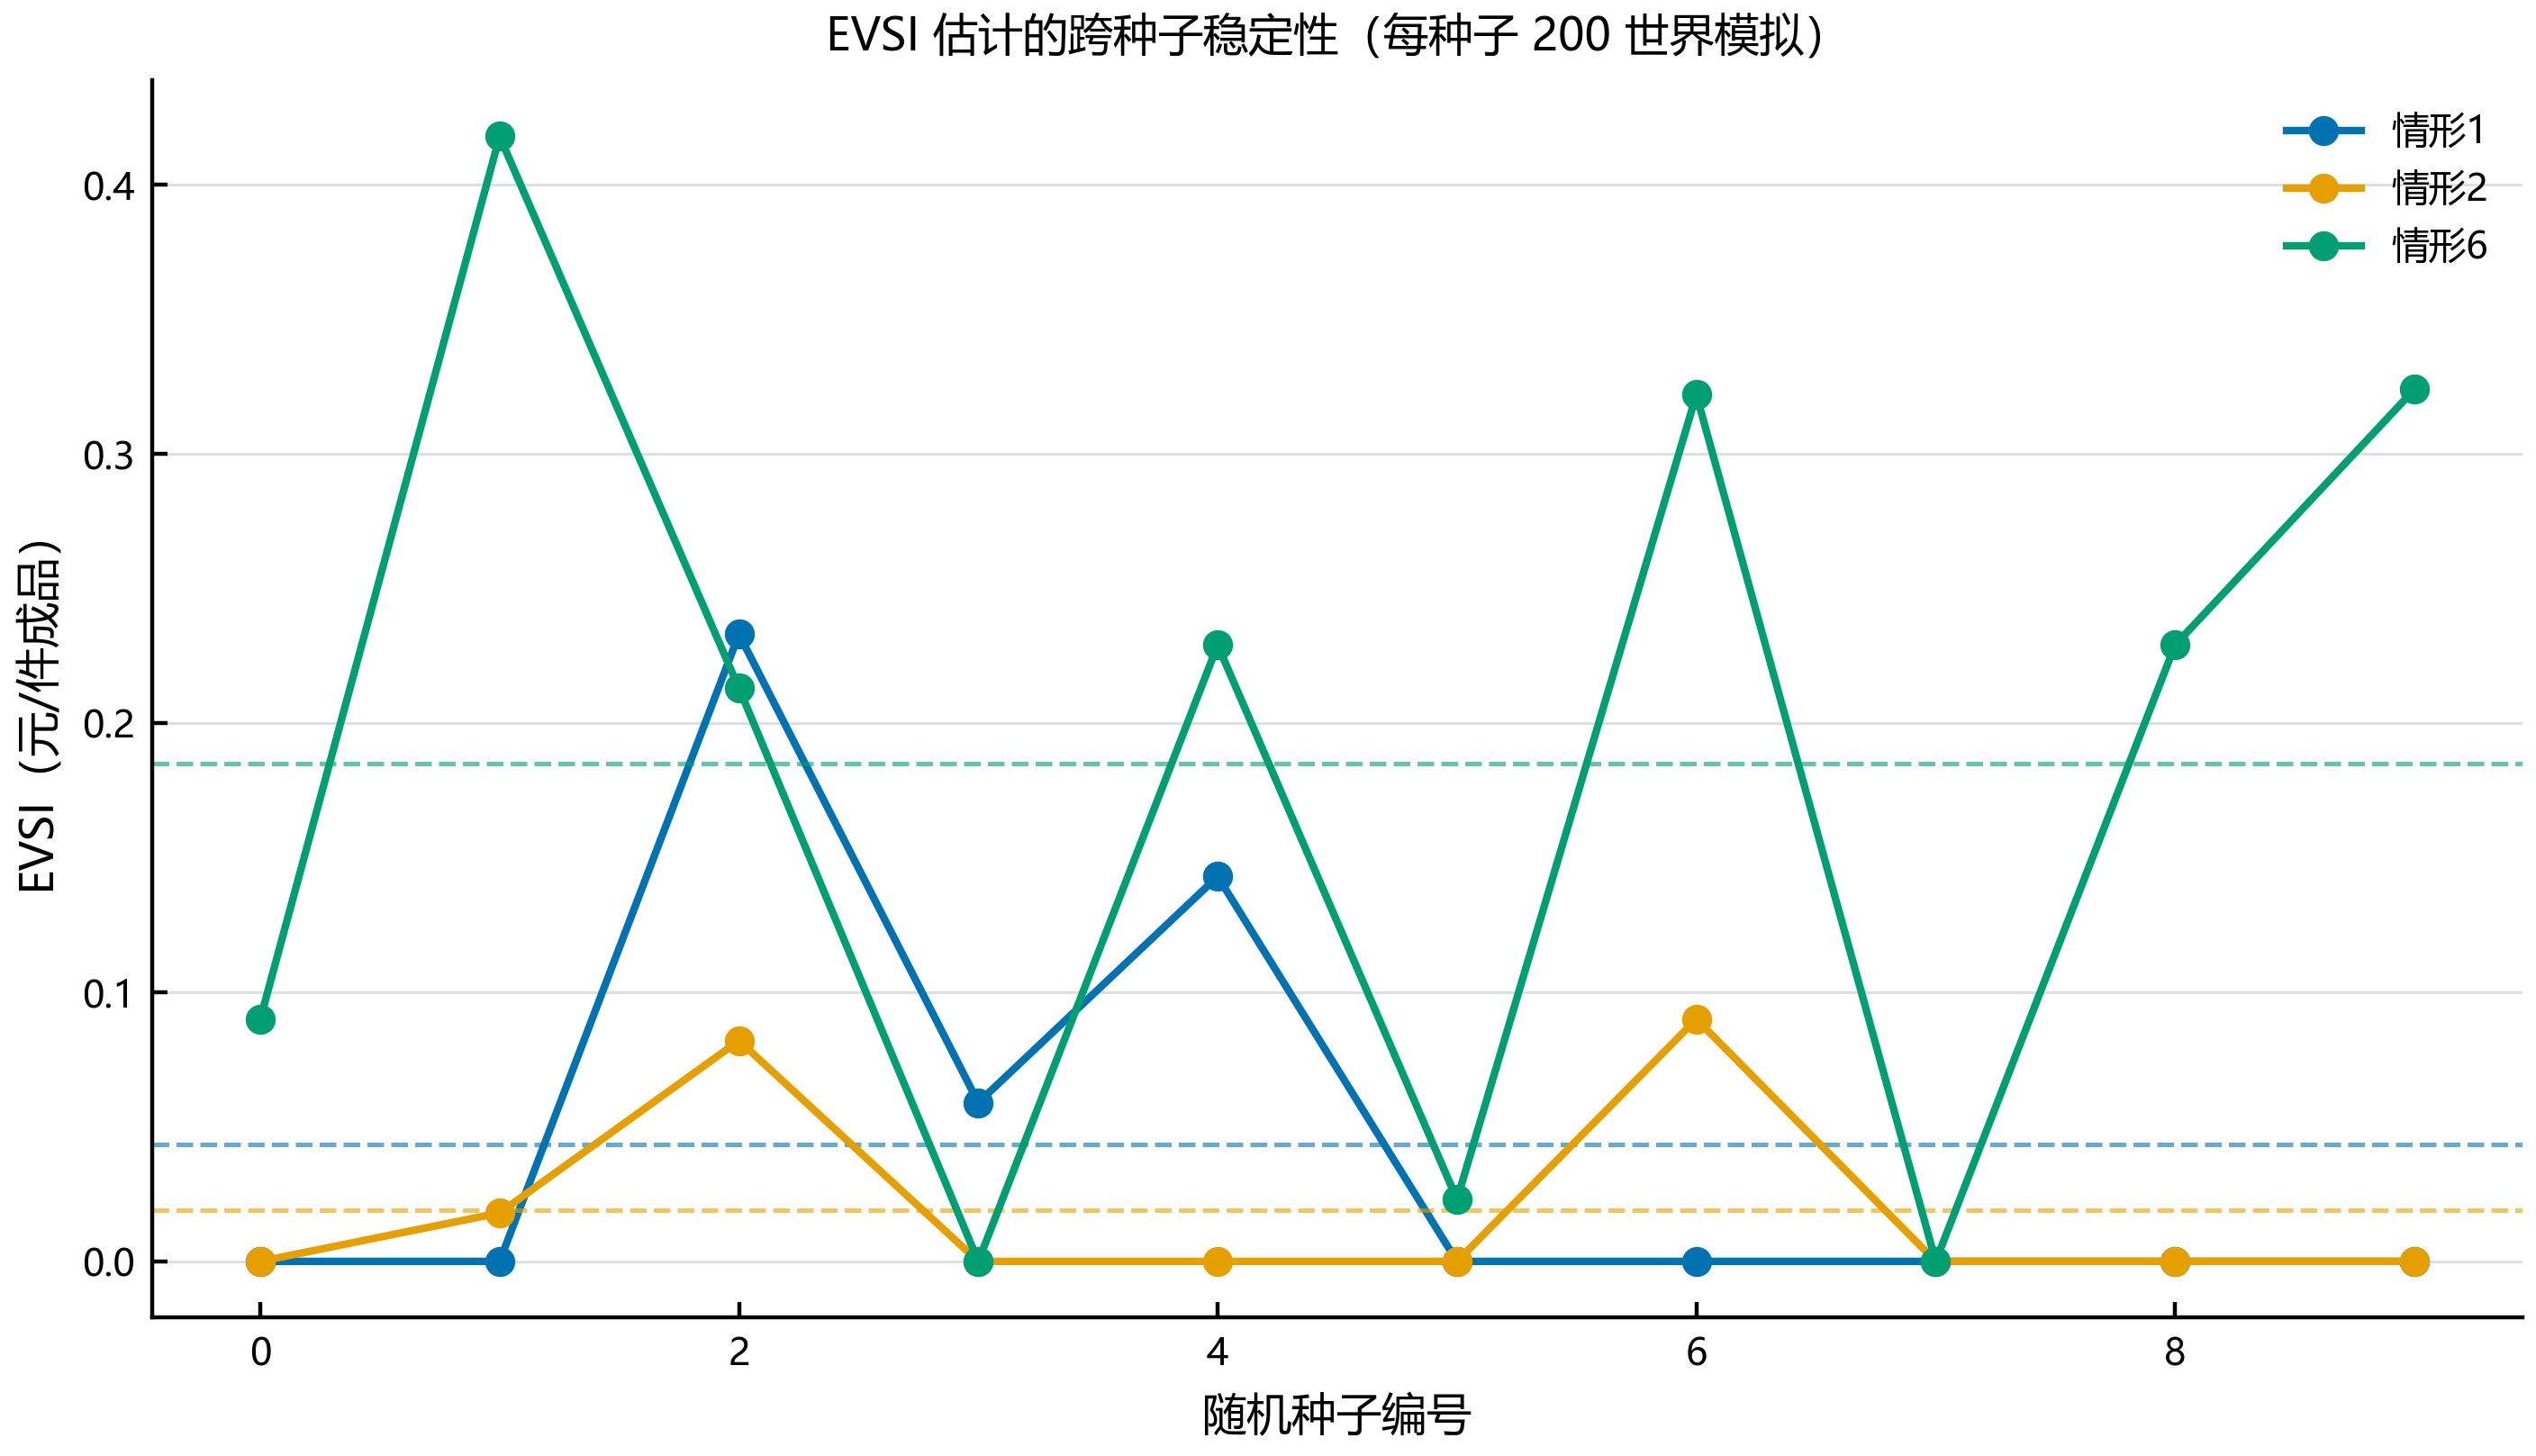
\includegraphics[width=0.85\textwidth]{fig6_evsi_stability.png}
    \caption{10 个随机种子下 EVSI 估计的稳定性。
    情形 6 的 EVSI（$0.185 \pm 0.149$ 元/件）显著高于
    情形 1（$0.044 \pm 0.081$）与情形 2（$0.019 \pm 0.036$），
    三种情形 EVSI 均值差异在数量级上稳定，与
    §5.4.3 单种子结论一致。}
    \label{fig:q4-evsi-stability}
\end{figure}

\begin{table}[htbp]
\centering
\caption{10 个种子下最优抽样量 $n^\star$ 与 EVSI 的统计}
\label{tab:q4-stability}
\small
\begin{tabular}{lccc}
\toprule[1.5pt]
情形 & $n^\star$ 范围 & $n^\star$ 均值 / 众数 &
$\mathrm{EVSI}$（元/件，均值 $\pm$ 标准差）\\
\midrule[1pt]
1 & $[0, 20]$   & 6.0 / 0  & $0.044 \pm 0.081$ \\
2 & $[0, 40]$   & 8.0 / 0  & $0.019 \pm 0.036$ \\
6 & $[0, 40]$   & 24.0 / 20 & $0.185 \pm 0.149$ \\
\bottomrule[1.5pt]
\end{tabular}
\end{table}

定性结论跨种子稳定：情形 6 的 EVSI 始终高于情形 1、2，量级
差异显著。定量上 $n^\star$ 在利润平台区间内波动（情形 1、2、6
的 $n^\star$ 分别落在 0--20、0--40、0--40），EVSI 均值的
标准差大于均值本身。波动的根源是 $V(n)$ 在最优附近平坦
（利润平台效应）：$n^\star$ 的具体值对随机数敏感，但所选
$n$ 对应的利润差可忽略。这与 §5.4.3 末段"决策翻转$\neq$
经济损失大"互证：抽样量的精确最优值不可靠，但"是否抽样"
与"抽样相对不抽样的相对量级"是稳健的。

\newpage

%% =====================================================================
%% 六、模型评价与推广
%% =====================================================================
\section{模型评价与推广}

\subsection{模型优点}

本文模型在方法、求解与验证层面均体现出较好的
体系性，主要优点可归纳为以下三点：

\begin{enumerate}
    \item \textbf{精确性}。问题 1 使用精确二项概率（无正态
    近似），问题 2、3 使用解析期望而非经验打分，问题 4 使用
    Beta--Binomial 共轭更新而非高斯近似，从而在同等计算成本
    下提高了结论的数值精度。
    \item \textbf{全局最优性}。当前规模下完整枚举 16 与
    65\,536 种策略；不存在初值依赖与局部最优陷阱，结果可
    严格复核。
    \item \textbf{体系一致}。问题 4 将抽样成本、后验信息
    与问题 2 利润函数连接起来，使"统计--决策--经济价值"
    在同一框架下可对比、可换算，回答了"问题 1 的抽样方案
    在经济上是否值得"的根本问题。
\end{enumerate}

\subsection{模型局限}

尽管本文模型在题目给定的参数范围内表现良好，但仍存在以下
三点局限：

\begin{enumerate}
    \item \textbf{检测无误差假设}。全文假设检测无误判、
    漏判，实际生产中检测设备存在灵敏度与特异度限制。
    \item \textbf{全枚举的复杂度爆炸}。问题 3 的 $2^{16}$
    枚举在配件数量 $n$ 显著增加（如 $n = 20$）后不可行，
    需转向动态规划、分支定界或启发式搜索。
    \item \textbf{问题 4 先验与批量的主观性}。Beta 先验
    的等价样本量 $n_{\mathrm{prior}} = 30$ 与批量 $B$ 均为
    外生假设，小 EVSI 场景对蒙特卡洛误差敏感。
\end{enumerate}

\subsection{推广方向}

针对上述局限，未来工作可从以下三个方向扩展：

\begin{enumerate}
    \item \textbf{检测误差建模}。引入灵敏度、特异度与复检
    机制，将本文零误差假设下的最优策略推广为考虑误检
    成本的鲁棒版本。
    \item \textbf{大规模网络的高效算法}。对一般有向无环
    图（DAG）形式的装配网络，用动态规划或消息传递算法
    自底向上聚合节点质量与期望成本；当决策变量进一步
    增多时，本文的级联递推结构恰好为这类方法提供了
    天然的状态聚合单元。
    \item \textbf{动态学习与在线更新}。将抽样从一次性静态
    决策扩展为逐批更新、贝叶斯控制图或序贯停止规则，
    使企业能够在生产过程中持续修正对供应商质量的认知。
\end{enumerate}

\newpage

%% =====================================================================
%% 参考文献
%% =====================================================================
\begin{thebibliography}{9}

\bibitem{tongji2007}
盛骤, 谢式千, 潘承毅.
概率论与数理统计（第四版）[M].
北京: 高等教育出版社, 2007.

\bibitem{degroot1970}
DeGroot M H.
\emph{Optimal Statistical Decisions}[M].
New York: McGraw-Hill, 1970.

\bibitem{howard1966}
Howard R A.
Information value theory[J].
\emph{IEEE Transactions on Systems Science and Cybernetics},
1966, 2(1): 22--26.

\bibitem{wald1945}
Wald A.
Sequential tests of statistical hypotheses[J].
\emph{The Annals of Mathematical Statistics},
1945, 16(2): 117--186.

\bibitem{metropolis1949}
Metropolis N, Ulam S.
The Monte Carlo method[J].
\emph{Journal of the American Statistical Association},
1949, 44(247): 335--341.

\bibitem{montgomery2013}
Montgomery D C.
\emph{Introduction to Statistical Quality Control}[M].
7th ed. New York: Wiley, 2013.

\bibitem{gb2828}
中华人民共和国国家标准.
计数抽样检验程序 第 1 部分：按接收质量限（AQL）检索的逐批
检验抽样计划：GB/T 2828.1—2012[S].
北京: 中国标准出版社, 2012.

\bibitem{raiffa1961}
Raiffa H, Schlaifer R.
\emph{Applied Statistical Decision Theory}[M].
Cambridge, MA: MIT Press, 1961.

\bibitem{bertsekas2005}
Bertsekas D P.
\emph{Dynamic Programming and Optimal Control}, Vol. I[M].
3rd ed. Belmont, MA: Athena Scientific, 2005.

\end{thebibliography}

\newpage

%% =====================================================================
%% 附录
%% =====================================================================
\begin{appendices}

\section{问题 1 SPRT 扩展}
\label{app:sprt}

Wald 序贯概率比检验（SPRT）可作为固定样本量方案的方法扩展。
设原假设 $H_0: p = p_0$ 与备择假设 $H_1: p = p_1$（取
$p_1 = 0.20$），给定第一类错误率 $\alpha$ 与第二类错误率 $\beta$，
序贯方案在观测到第 $m$ 件时停止采样并作判定：

\begin{itemize}
    \item 当对数似然比
    $\lambda_m = \sum_{i=1}^{m} \log \frac{f_1(X_i)}{f_0(X_i)}
    \geq \log \frac{1 - \beta}{\alpha}$ 时，判定拒收
    （接受 $H_1$）；
    \item 当 $\lambda_m \leq \log \frac{\beta}{1 - \alpha}$ 时，
    判定接收（接受 $H_0$）；
    \item 否则继续抽样。
\end{itemize}

通过蒙特卡洛模拟比较固定方案与 SPRT 方案可见：
\begin{itemize}
    \item 在 $p$ 明显优于或劣于 $p_0$ 的区域，SPRT 平均抽样
    次数显著小于固定方案；
    \item 在 $p$ 接近 $p_0$ 的难判区域，SPRT 的期望抽样次数
    可能高于固定方案（$n = 29$ 或 $n = 22$）；
    \item SPRT 复杂度更高、需要事先指定 $p_1$ 与两类错误率，
    不符合题面"以尽量少的抽检次数决定是否接收"的最简化要求，
    故不作为主方法。
\end{itemize}

\clearpage

\section{问题 2 完整 16 策略表}

\begin{table}[htbp]
\centering
\caption{问题 2 六种情形 $\times$ 16 策略期望利润（单位：元/件）}
\label{app:tab-q2-all}
\small
\begin{adjustbox}{width=\textwidth}
\begin{tabular}{@{}lcccccc@{}}
\toprule[1.5pt]
策略 $(x_1x_2x_3x_4)$ & 情形 1 & 情形 2 & 情形 3 & 情形 4 & 情形 5 & 情形 6 \\
\midrule[1pt]
\texttt{0000} & 16.78 & 6.92  & 16.78 & 9.81  & 16.41 & \textbf{21.68} \\
\texttt{0001} & \textbf{21.68} & 12.85 & 19.66 & 14.95 & 18.79 & 14.84 \\
\texttt{0010} & 19.66 & 10.95 & 19.66 & 13.05 & 19.50 & 18.29 \\
\texttt{0011} & 21.46 & 12.70 & \textbf{19.80} & 14.92 & \textbf{18.94} & 16.85 \\
\texttt{0100} & 11.99 & 4.81  & 11.99 & 7.50  & 11.40 & 17.20 \\
\texttt{0101} & 16.95 & 8.32  & 14.83 & 11.02 & 13.78 & 13.21 \\
\texttt{0110} & 14.83 & 8.32  & 14.83 & 10.97 & 14.50 & 13.79 \\
\texttt{0111} & 16.62 & 10.04 & 14.91 & 12.74 & 13.88 & 12.62 \\
\texttt{1000} & 15.30 & 11.83 & 15.30 & 14.71 & 14.92 & 20.20 \\
\texttt{1001} & 20.13 & \textbf{12.97} & 18.05 & \textbf{15.17} & 17.10 & 13.36 \\
\texttt{1010} & 18.05 & 11.78 & 18.05 & 14.89 & 18.06 & 16.81 \\
\texttt{1011} & 19.85 & 12.79 & 18.16 & 15.10 & 17.51 & 14.38 \\
\texttt{1100} & 10.51 & 9.72  & 10.51 & 12.40 & 9.91  & 15.72 \\
\texttt{1101} & 15.40 & 13.21 & 13.20 & 15.93 & 12.23 & 11.74 \\
\texttt{1110} & 13.27 & 13.21 & 13.27 & 15.97 & 12.96 & 12.32 \\
\texttt{1111} & 14.96 & 14.89 & 13.30 & 17.59 & 12.27 & 11.13 \\
\bottomrule[1.5pt]
\end{tabular}
\end{adjustbox}
\end{table}

\clearpage

\section{问题 3 等价最优编码}

\begin{table}[htbp]
\centering
\small
\begin{tabular}{ll}
\toprule[1.5pt]
\textbf{规范编码} & \textbf{备注} \\
\midrule[1pt]
\texttt{11111111|000|000|11} & 规范代表编码 \\
\texttt{11111111|000|001|11} & $z_1$ 不触发 \\
\texttt{11111111|000|010|11} & $z_2$ 不触发 \\
\texttt{11111111|000|011|11} & $z_1 z_2$ 不触发 \\
\texttt{11111111|000|100|11} & $z_3$ 不触发 \\
\texttt{11111111|000|101|11} & $z_1 z_3$ 不触发 \\
\texttt{11111111|000|110|11} & $z_2 z_3$ 不触发 \\
\texttt{11111111|000|111|11} & $z_1 z_2 z_3$ 均不触发 \\
\bottomrule[1.5pt]
\end{tabular}
\end{table}

\section{问题 4 观测—决策表示例}
\label{app:q4-table}

表 \ref{app:tab-q4} 给出问题 4 情形 2 下若干代表性观测对应的
最优策略（先验 $\hat p_1 = \hat p_2 = \hat p_0 = 0.10$，
$n_{\mathrm{prior}} = 30$，$n = 10$）。

\begin{table}[htbp]
\centering
\caption{问题 4 情形 2 观测—决策表示例}
\label{app:tab-q4}
\small
\begin{tabular}{ccccl}
\toprule[1.5pt]
$k_1$ & $k_2$ & $k_0$ & $x^\star$ & 说明 \\
\midrule[1pt]
0 & 0 & 0 & 0000 & 观测偏乐观，决策偏不检测 \\
1 & 1 & 1 & 1001 & 中等观测，开启配件 1 检测 \\
2 & 2 & 2 & 1011 & 高观测，前端与成品检测并拆解 \\
3 & 3 & 3 & 1111 & 极高观测，全检全拆 \\
\bottomrule[1.5pt]
\end{tabular}
\end{table}

\section{主要算法源码}

本节附录贴出三个问题的核心求解代码片段。

\subsection{问题 2：两零配件生产决策核心代码}

仅展示策略评估核心函数 \texttt{eval\_strategy}。

\lstinputlisting[linerange={53-105}, firstnumber=53,
               title={\texttt{p2/p2\_solver.py}（53--105 行）}]
              {../p2/p2_solver.py}

\subsection{问题 3：多级装配级联递推核心代码}

仅展示策略评估核心函数 \texttt{eval\_strategy}。

\lstinputlisting[linerange={44-76}, firstnumber=44,
               title={\texttt{p3/p3\_solver.py}（44--76 行）}]
              {../p3/p3_solver.py}

\subsection{问题 4：EVSI 核心代码}

仅展示 \texttt{profit\_vec} 与 \texttt{V\_all\_n} 两个核心函数
。

\lstinputlisting[linerange={54-73,88-107}, firstnumber=54,
               title={\texttt{p4/p4\_evsi.py}（54--73, 88--107 行）}]
              {../p4/p4_evsi.py}

\end{appendices}

\end{document}
